% Options for packages loaded elsewhere
\PassOptionsToPackage{unicode}{hyperref}
\PassOptionsToPackage{hyphens}{url}
\PassOptionsToPackage{dvipsnames,svgnames,x11names}{xcolor}
%
\documentclass[
  12pt,
]{book}
\usepackage{amsmath,amssymb}
\usepackage{iftex}
\ifPDFTeX
  \usepackage[T1]{fontenc}
  \usepackage[utf8]{inputenc}
  \usepackage{textcomp} % provide euro and other symbols
\else % if luatex or xetex
  \usepackage{unicode-math} % this also loads fontspec
  \defaultfontfeatures{Scale=MatchLowercase}
  \defaultfontfeatures[\rmfamily]{Ligatures=TeX,Scale=1}
\fi
\usepackage{lmodern}
\ifPDFTeX\else
  % xetex/luatex font selection
\fi
% Use upquote if available, for straight quotes in verbatim environments
\IfFileExists{upquote.sty}{\usepackage{upquote}}{}
\IfFileExists{microtype.sty}{% use microtype if available
  \usepackage[]{microtype}
  \UseMicrotypeSet[protrusion]{basicmath} % disable protrusion for tt fonts
}{}
\makeatletter
\@ifundefined{KOMAClassName}{% if non-KOMA class
  \IfFileExists{parskip.sty}{%
    \usepackage{parskip}
  }{% else
    \setlength{\parindent}{0pt}
    \setlength{\parskip}{6pt plus 2pt minus 1pt}}
}{% if KOMA class
  \KOMAoptions{parskip=half}}
\makeatother
\usepackage{xcolor}
\usepackage[margin = 3cm]{geometry}
\usepackage{color}
\usepackage{fancyvrb}
\newcommand{\VerbBar}{|}
\newcommand{\VERB}{\Verb[commandchars=\\\{\}]}
\DefineVerbatimEnvironment{Highlighting}{Verbatim}{commandchars=\\\{\}}
% Add ',fontsize=\small' for more characters per line
\usepackage{framed}
\definecolor{shadecolor}{RGB}{248,248,248}
\newenvironment{Shaded}{\begin{snugshade}}{\end{snugshade}}
\newcommand{\AlertTok}[1]{\textcolor[rgb]{0.94,0.16,0.16}{#1}}
\newcommand{\AnnotationTok}[1]{\textcolor[rgb]{0.56,0.35,0.01}{\textbf{\textit{#1}}}}
\newcommand{\AttributeTok}[1]{\textcolor[rgb]{0.13,0.29,0.53}{#1}}
\newcommand{\BaseNTok}[1]{\textcolor[rgb]{0.00,0.00,0.81}{#1}}
\newcommand{\BuiltInTok}[1]{#1}
\newcommand{\CharTok}[1]{\textcolor[rgb]{0.31,0.60,0.02}{#1}}
\newcommand{\CommentTok}[1]{\textcolor[rgb]{0.56,0.35,0.01}{\textit{#1}}}
\newcommand{\CommentVarTok}[1]{\textcolor[rgb]{0.56,0.35,0.01}{\textbf{\textit{#1}}}}
\newcommand{\ConstantTok}[1]{\textcolor[rgb]{0.56,0.35,0.01}{#1}}
\newcommand{\ControlFlowTok}[1]{\textcolor[rgb]{0.13,0.29,0.53}{\textbf{#1}}}
\newcommand{\DataTypeTok}[1]{\textcolor[rgb]{0.13,0.29,0.53}{#1}}
\newcommand{\DecValTok}[1]{\textcolor[rgb]{0.00,0.00,0.81}{#1}}
\newcommand{\DocumentationTok}[1]{\textcolor[rgb]{0.56,0.35,0.01}{\textbf{\textit{#1}}}}
\newcommand{\ErrorTok}[1]{\textcolor[rgb]{0.64,0.00,0.00}{\textbf{#1}}}
\newcommand{\ExtensionTok}[1]{#1}
\newcommand{\FloatTok}[1]{\textcolor[rgb]{0.00,0.00,0.81}{#1}}
\newcommand{\FunctionTok}[1]{\textcolor[rgb]{0.13,0.29,0.53}{\textbf{#1}}}
\newcommand{\ImportTok}[1]{#1}
\newcommand{\InformationTok}[1]{\textcolor[rgb]{0.56,0.35,0.01}{\textbf{\textit{#1}}}}
\newcommand{\KeywordTok}[1]{\textcolor[rgb]{0.13,0.29,0.53}{\textbf{#1}}}
\newcommand{\NormalTok}[1]{#1}
\newcommand{\OperatorTok}[1]{\textcolor[rgb]{0.81,0.36,0.00}{\textbf{#1}}}
\newcommand{\OtherTok}[1]{\textcolor[rgb]{0.56,0.35,0.01}{#1}}
\newcommand{\PreprocessorTok}[1]{\textcolor[rgb]{0.56,0.35,0.01}{\textit{#1}}}
\newcommand{\RegionMarkerTok}[1]{#1}
\newcommand{\SpecialCharTok}[1]{\textcolor[rgb]{0.81,0.36,0.00}{\textbf{#1}}}
\newcommand{\SpecialStringTok}[1]{\textcolor[rgb]{0.31,0.60,0.02}{#1}}
\newcommand{\StringTok}[1]{\textcolor[rgb]{0.31,0.60,0.02}{#1}}
\newcommand{\VariableTok}[1]{\textcolor[rgb]{0.00,0.00,0.00}{#1}}
\newcommand{\VerbatimStringTok}[1]{\textcolor[rgb]{0.31,0.60,0.02}{#1}}
\newcommand{\WarningTok}[1]{\textcolor[rgb]{0.56,0.35,0.01}{\textbf{\textit{#1}}}}
\usepackage{longtable,booktabs,array}
\usepackage{calc} % for calculating minipage widths
% Correct order of tables after \paragraph or \subparagraph
\usepackage{etoolbox}
\makeatletter
\patchcmd\longtable{\par}{\if@noskipsec\mbox{}\fi\par}{}{}
\makeatother
% Allow footnotes in longtable head/foot
\IfFileExists{footnotehyper.sty}{\usepackage{footnotehyper}}{\usepackage{footnote}}
\makesavenoteenv{longtable}
\usepackage{graphicx}
\makeatletter
\def\maxwidth{\ifdim\Gin@nat@width>\linewidth\linewidth\else\Gin@nat@width\fi}
\def\maxheight{\ifdim\Gin@nat@height>\textheight\textheight\else\Gin@nat@height\fi}
\makeatother
% Scale images if necessary, so that they will not overflow the page
% margins by default, and it is still possible to overwrite the defaults
% using explicit options in \includegraphics[width, height, ...]{}
\setkeys{Gin}{width=\maxwidth,height=\maxheight,keepaspectratio}
% Set default figure placement to htbp
\makeatletter
\def\fps@figure{htbp}
\makeatother
\setlength{\emergencystretch}{3em} % prevent overfull lines
\providecommand{\tightlist}{%
  \setlength{\itemsep}{0pt}\setlength{\parskip}{0pt}}
\setcounter{secnumdepth}{5}
\ifLuaTeX
\usepackage[bidi=basic]{babel}
\else
\usepackage[bidi=default]{babel}
\fi
\babelprovide[main,import]{english}
% get rid of language-specific shorthands (see #6817):
\let\LanguageShortHands\languageshorthands
\def\languageshorthands#1{}
\usepackage{booktabs}
\usepackage{mathrsfs}
\usepackage{amsmath}
\usepackage[spanish, spanishkw, onelanguage, linesnumbered]{algorithm2e}
\usepackage{ragged2e}
\AtBeginDocument{\justifying}
\usepackage{booktabs}
\usepackage{longtable}
\usepackage{array}
\usepackage{multirow}
\usepackage{wrapfig}
\usepackage{float}
\usepackage{colortbl}
\usepackage{pdflscape}
\usepackage{tabu}
\usepackage{threeparttable}
\usepackage{threeparttablex}
\usepackage[normalem]{ulem}
\usepackage{makecell}
\usepackage{xcolor}
\ifLuaTeX
  \usepackage{selnolig}  % disable illegal ligatures
\fi
\usepackage[]{natbib}
\bibliographystyle{apalike}
\IfFileExists{bookmark.sty}{\usepackage{bookmark}}{\usepackage{hyperref}}
\IfFileExists{xurl.sty}{\usepackage{xurl}}{} % add URL line breaks if available
\urlstyle{same}
\hypersetup{
  pdftitle={Area models for estimating poverty and labor market indicators},
  pdfauthor={Andrés Gutiérrez, Stalyn Guerrero, Gabriel Nieto},
  pdflang={en},
  colorlinks=true,
  linkcolor={blue},
  filecolor={Maroon},
  citecolor={Blue},
  urlcolor={Blue},
  pdfcreator={LaTeX via pandoc}}

\title{Area models for estimating poverty and labor market indicators}
\author{Andrés Gutiérrez\footnote{Experto Regional en Estadísticas Sociales - Comisión Económica para América Latina y el Caribe (CEPAL) - \href{mailto:andres.gutierrez@cepal.org}{\nolinkurl{andres.gutierrez@cepal.org}}}, Stalyn Guerrero\footnote{Consultor - Comisión Económica para América Latina y el Caribe (CEPAL) - \href{mailto:guerrerostalyn@gmail.com}{\nolinkurl{guerrerostalyn@gmail.com}}}, Gabriel Nieto\footnote{Consultor - Comisión Económica para América Latina y el Caribe (CEPAL) - \href{mailto:gabrieljose.nieto@gmail.com}{\nolinkurl{gabrieljose.nieto@gmail.com}}}}
\date{2023-12-14}

\begin{document}
\maketitle

{
\hypersetup{linkcolor=}
\setcounter{tocdepth}{1}
\tableofcontents
}
\listoffigures
\listoftables
\hypertarget{workshop-material}{%
\chapter*{Workshop material}\label{workshop-material}}
\addcontentsline{toc}{chapter}{Workshop material}

\hypertarget{workshop-material-1}{%
\section*{Workshop material}\label{workshop-material-1}}
\addcontentsline{toc}{section}{Workshop material}

In the following link you will find the R routines developed for the workshop.
\href{https://github.com/stalynGuerrero/2023JAMSae/}{Download}

\hypertarget{session-1--census-and-satellite-information}{%
\chapter{Session 1- Census and satellite information}\label{session-1--census-and-satellite-information}}

\hypertarget{use-of-satellite-imagery-and-sae}{%
\section{Use of Satellite Imagery and SAE}\label{use-of-satellite-imagery-and-sae}}

One of the pioneering articles in small area estimation was the paper by Singh, R, et al.~(2002), which addressed crop yield estimation for the tehsils (sub-administrative units) of Rohtak district in Haryana, India.

Raster images represent the world through a set of contiguous equally spaced cells known as pixels. These images contain information like a geographic information system and a coordinate reference system. Images store an identifier, a value in each pixel (or a vector with different values), and each cell is associated with a color scale.

Images can be obtained in raw and processed forms. The former contains only color layers, while the latter also contains values that have been processed in each cell (vegetation indices, light intensity, type of vegetation).

Raw information can be used to train desired features (roads, crop types, forest/non-forest). Fortunately, in Google Earth Engine, we find many processed indicators associated with a pixel. These indicators can be aggregated at a geographical area level.

\hypertarget{satellite-image-data-sources}{%
\section{Satellite Image Data Sources}\label{satellite-image-data-sources}}

Some of the main sources of satellite images include:

\begin{itemize}
\item
  \href{http://earthexplorer.usgs.gov/}{USGS Earth Explorer}
\item
  \href{https://lpdaacsvc.cr.usgs.gov/appeears/}{Land Processes Distributed Active Archive Center (LP DAAC)}
\item
  \href{https://search.earthdata.nasa.gov/search}{NASA Earthdata Search}
\item
  \href{https://scihub.copernicus.eu/}{Copernicus Open Access Hub}
\item
  \href{https://aws.amazon.com/public-data-sets/landsat/}{AWS Public Dataset - Landsat}
\end{itemize}

However, most of these sources are centralized within \textbf{Google Earth Engine}, which allows searching for satellite image data sources. GEE can be managed through APIs in different programming languages: JavaScript (by default), Python, and R (rgee package).

\hypertarget{google-earth-engine}{%
\section{Google Earth Engine}\label{google-earth-engine}}

Create an account at \href{https://earthengine.google.com/}{this link}. Once logged in, you can search for datasets of interest:

\begin{figure}
\centering
\includegraphics{Recursos/01_Session1/01_lights.png}
\caption{Night Lights Image}
\end{figure}

\begin{itemize}
\item
  Upon searching for the dataset, you can open a code editor provided by Google in JavaScript.
\item
  Copy and paste the syntax provided by the dataset search to visualize the raster image and obtain statements allowing for the retrieval of the dataset of interest later in R.
\end{itemize}

\begin{figure}
\centering
\includegraphics{Recursos/01_Session1/02_query.png}
\caption{Syntax in JavaScript}
\end{figure}

\hypertarget{installing-rgee}{%
\section{Installing rgee}\label{installing-rgee}}

\begin{itemize}
\item
  Download and install Anaconda or Conda from \href{https://www.anaconda.com/products/individual}{here}.
\item
  Open \textbf{Anaconda Prompt} and set up a working environment (Python environment JAM2023) using the following commands:
\end{itemize}

\begin{verbatim}
conda env list
conda create -n JAM2023 python=3.9
activate JAM2023
pip install google-api-python-client
pip install earthengine-api
pip install numpy
\end{verbatim}

\begin{itemize}
\tightlist
\item
  List available Python environments in Anaconda Prompt:
\end{itemize}

\begin{verbatim}
conda env list
\end{verbatim}

\begin{itemize}
\tightlist
\item
  Once you've identified the path of the JAM2023 environment, set it in R (\textbf{remember to change \textbackslash{} to /}).
\item
  Install \texttt{reticulate} and \texttt{rgee}, load packages for spatial processing, and set up the working environment as follows:
\end{itemize}

\begin{Shaded}
\begin{Highlighting}[]
\FunctionTok{library}\NormalTok{(reticulate) }\CommentTok{\# Connection with Python}
\FunctionTok{library}\NormalTok{(rgee) }\CommentTok{\# Connection with Google Earth Engine}
\FunctionTok{library}\NormalTok{(sf) }\CommentTok{\# Package for handling geographic data}
\FunctionTok{library}\NormalTok{(dplyr) }\CommentTok{\# Package for data processing}
\FunctionTok{library}\NormalTok{(magrittr)}

\NormalTok{rgee\_environment\_dir }\OtherTok{=} \StringTok{"C:/Users/gnieto/Anaconda3/envs/JAM2023/python.exe"}

\CommentTok{\# Set up Python (Sometimes not detected and R needs to be restarted)}
\NormalTok{reticulate}\SpecialCharTok{::}\FunctionTok{use\_python}\NormalTok{(rgee\_environment\_dir, }\AttributeTok{required=}\NormalTok{T)}

\NormalTok{rgee}\SpecialCharTok{::}\FunctionTok{ee\_install\_set\_pyenv}\NormalTok{(}\AttributeTok{py\_path =}\NormalTok{ rgee\_environment\_dir, }\AttributeTok{py\_env =} \StringTok{"JAM2023"}\NormalTok{)}

\FunctionTok{Sys.setenv}\NormalTok{(}\AttributeTok{RETICULATE\_PYTHON =}\NormalTok{ rgee\_environment\_dir)}
\FunctionTok{Sys.setenv}\NormalTok{(}\AttributeTok{EARTHENGINE\_PYTHON =}\NormalTok{ rgee\_environment\_dir)}
\end{Highlighting}
\end{Shaded}

\begin{itemize}
\tightlist
\item
  Once the environment is configured, you can initialize a Google Earth Engine session as follows:
\end{itemize}

\begin{Shaded}
\begin{Highlighting}[]
\NormalTok{rgee}\SpecialCharTok{::}\FunctionTok{ee\_Initialize}\NormalTok{(}\AttributeTok{drive =}\NormalTok{ T)}
\end{Highlighting}
\end{Shaded}

\begin{figure}
\centering
\includegraphics{Recursos/01_Session1/03_Figura.PNG}
\caption{Session started successfully}
\end{figure}

\textbf{Notes:}

\begin{itemize}
\item
  Each session must be initialized with the command \texttt{rgee::ee\_Initialize(drive\ =\ T)}.
\item
  JavaScript commands invoking methods with ``.'' are replaced by the dollar sign (\$), for example:
\end{itemize}

\begin{Shaded}
\begin{Highlighting}[]
\FunctionTok{ee.ImageCollection}\NormalTok{()}\FunctionTok{.filterDate}\NormalTok{()  }\CommentTok{\# JavaScript}
\NormalTok{ee}\SpecialCharTok{$}\FunctionTok{ImageCollection}\NormalTok{()}\SpecialCharTok{$}\FunctionTok{filterDate}\NormalTok{()  }\CommentTok{\# R}
\end{Highlighting}
\end{Shaded}

\hypertarget{downloading-satellite-information}{%
\subsection{Downloading Satellite Information}\label{downloading-satellite-information}}

\begin{itemize}
\tightlist
\item
  \textbf{Step 1}: Have the shapefiles ready.
\end{itemize}

\begin{Shaded}
\begin{Highlighting}[]
\NormalTok{shape }\OtherTok{\textless{}{-}} \FunctionTok{read\_sf}\NormalTok{(}\StringTok{"Shapefile/JAM2\_cons.shp"}\NormalTok{) }
\FunctionTok{plot}\NormalTok{(shape[}\StringTok{"geometry"}\NormalTok{])}
\end{Highlighting}
\end{Shaded}

\begin{figure}
\centering
\includegraphics{Recursos/01_Session1/04_JAM.PNG}
\caption{Shapefile}
\end{figure}

\begin{itemize}
\tightlist
\item
  \textbf{Step 2}: Select the image file you want to process, for example, \textbf{night lights}.
\end{itemize}

\begin{Shaded}
\begin{Highlighting}[]
\NormalTok{lights }\OtherTok{\textless{}{-}}\NormalTok{ ee}\SpecialCharTok{$}\FunctionTok{ImageCollection}\NormalTok{(}\StringTok{"NOAA/DMSP{-}OLS/NIGHTTIME\_LIGHTS"}\NormalTok{) }\SpecialCharTok{\%\textgreater{}\%}
\NormalTok{  ee}\SpecialCharTok{$}\NormalTok{ImageCollection}\SpecialCharTok{$}\FunctionTok{filterDate}\NormalTok{(}\StringTok{"2013{-}01{-}01"}\NormalTok{, }\StringTok{"2014{-}01{-}01"}\NormalTok{) }\SpecialCharTok{\%\textgreater{}\%}
\NormalTok{  ee}\SpecialCharTok{$}\NormalTok{ImageCollection}\SpecialCharTok{$}\FunctionTok{map}\NormalTok{(}\ControlFlowTok{function}\NormalTok{(x) x}\SpecialCharTok{$}\FunctionTok{select}\NormalTok{(}\StringTok{"stable\_lights"}\NormalTok{)) }\SpecialCharTok{\%\textgreater{}\%}
\NormalTok{  ee}\SpecialCharTok{$}\NormalTok{ImageCollection}\SpecialCharTok{$}\FunctionTok{toBands}\NormalTok{()}
\end{Highlighting}
\end{Shaded}

\begin{itemize}
\tightlist
\item
  \textbf{Step 3}: Download the information.
\end{itemize}

\begin{Shaded}
\begin{Highlighting}[]
\DocumentationTok{\#\# Takes about 10 minutes }
\NormalTok{lights\_shape }\OtherTok{\textless{}{-}} \FunctionTok{map}\NormalTok{(}\FunctionTok{unique}\NormalTok{(shape}\SpecialCharTok{$}\NormalTok{dam2),}
                 \SpecialCharTok{\textasciitilde{}}\FunctionTok{tryCatch}\NormalTok{(}\FunctionTok{ee\_extract}\NormalTok{(}
                   \AttributeTok{x =}\NormalTok{ lights,}
                   \AttributeTok{y =}\NormalTok{ shape[}\StringTok{"dam2"}\NormalTok{] }\SpecialCharTok{\%\textgreater{}\%} \FunctionTok{filter}\NormalTok{(dam2 }\SpecialCharTok{==}\NormalTok{ .x),}
\NormalTok{                   ee}\SpecialCharTok{$}\NormalTok{Reducer}\SpecialCharTok{$}\FunctionTok{mean}\NormalTok{(),}
                   \AttributeTok{sf =} \ConstantTok{FALSE}
\NormalTok{                 ) }\SpecialCharTok{\%\textgreater{}\%} \FunctionTok{mutate}\NormalTok{(}\AttributeTok{dam2 =}\NormalTok{ .x),}
                 \AttributeTok{error =} \ControlFlowTok{function}\NormalTok{(e)}\FunctionTok{data.frame}\NormalTok{(}\AttributeTok{dam2 =}\NormalTok{ .x)))}

\NormalTok{lights\_shape }\SpecialCharTok{\%\textless{}\textgreater{}\%} \FunctionTok{bind\_rows}\NormalTok{()}

\FunctionTok{tba}\NormalTok{(lights\_shape, }\AttributeTok{cap =} \StringTok{"Average of night lights"}\NormalTok{)}
\end{Highlighting}
\end{Shaded}

\begin{table}[H]

\caption{\label{tab:unnamed-chunk-7}Average standardized night lights}
\centering
\begin{tabu} to \linewidth {>{\raggedright}X>{\raggedleft}X}
\toprule
dam2 & stable\_lights\_mean\\
\midrule
0101 & 0.9393\\
0102 & 1.6857\\
0103 & 1.6900\\
0201 & -0.4380\\
0202 & 1.4627\\
\addlinespace
0203 & 1.3519\\
0204 & 1.6333\\
0205 & 1.7522\\
0206 & 1.7522\\
0207 & 1.7444\\
\bottomrule
\end{tabu}
\end{table}

Repeat the routine for:

\begin{itemize}
\item
  Soil type: \textbf{crops-coverfraction} (Percentage of crop cover) and \textbf{urban-coverfraction} (Percentage of urban cover) available at \url{https://developers.google.com/earth-engine/datasets/catalog/COPERNICUS_Landcover_100m_Proba-V-C3_Global\#description}
\item
  Travel time to the nearest hospital or clinic (\textbf{accessibility}) and travel time to the nearest hospital or clinic using non-motorized transport (\textbf{accessibility\_walking\_only}) information available at \url{https://developers.google.com/earth-engine/datasets/catalog/Oxford_MAP_accessibility_to_healthcare_2019}
\item
  Human modification, considering human settlements, agriculture, transportation, mining, energy production, and electrical infrastructure. You can find satellite information at the following link: \url{https://developers.google.com/earth-engine/datasets/catalog/CSP_HM_GlobalHumanModification\#description}
\item
  \textbf{Paso 4}: Consolidate the information.
\end{itemize}

\begin{table}[H]

\caption{\label{tab:unnamed-chunk-8}Standardized satellite predictors}
\centering
\begin{tabu} to \linewidth {>{\raggedright}X>{\raggedleft}X>{\raggedleft}X}
\toprule
dam2 & stable\_lights\_mean & crops.coverfraction\_mean\\
\midrule
0101 & 0.9393 & -0.5459\\
0102 & 1.6857 & -0.7090\\
0103 & 1.6900 & -0.3571\\
0201 & -0.4380 & -0.0874\\
0202 & 1.4627 & -0.6237\\
\addlinespace
0203 & 1.3519 & -0.6402\\
0204 & 1.6333 & -0.5050\\
0205 & 1.7522 & -0.6844\\
0206 & 1.7522 & -0.4289\\
0207 & 1.7444 & -0.4662\\
\bottomrule
\end{tabu}
\end{table}

\begin{figure}
\centering
\includegraphics{Recursos/01_Session1/06_stable_lights_sum.png}
\caption{Night Lights Sum}
\end{figure}

\begin{figure}
\centering
\includegraphics{Recursos/01_Session1/07_Luces_nocturnas.PNG}
\caption{Night Lights Satellite}
\end{figure}

\begin{figure}
\centering
\includegraphics{Recursos/01_Session1/08_crops.coverfraction_sum.png}
\caption{Crop Cover}
\end{figure}

\begin{figure}
\centering
\includegraphics{Recursos/01_Session1/09_Suelo_cultivo.PNG}
\caption{Crop Cover Satellite}
\end{figure}

\begin{figure}
\centering
\includegraphics{Recursos/01_Session1/10_urban.coverfraction_sum.png}
\caption{Urban Cover Sum}
\end{figure}

\begin{figure}
\centering
\includegraphics{Recursos/01_Session1/11_Suelo_urbano.PNG}
\caption{Urban Cover Satellite}
\end{figure}

\begin{figure}
\centering
\includegraphics{Recursos/01_Session1/12_gHM_sum.png}
\caption{Human Modification Sum}
\end{figure}

\begin{figure}
\centering
\includegraphics{Recursos/01_Session1/13_Modificación_humana.PNG}
\caption{Human Modification Satellite}
\end{figure}

\begin{figure}
\centering
\includegraphics{Recursos/01_Session1/14_accessibility_sum.png}
\caption{Average Travel Time to Hospital Sum}
\end{figure}

\begin{figure}
\centering
\includegraphics{Recursos/01_Session1/15_Distancia_Hospitales.PNG}
\caption{Average Travel Time to Hospital Satellite}
\end{figure}

\begin{figure}
\centering
\includegraphics{Recursos/01_Session1/16_accessibility_walking_only_mean.png}
\caption{Average Travel Time to Hospital by Non-Motorized Vehicle Sum}
\end{figure}

\begin{figure}
\centering
\includegraphics{Recursos/01_Session1/17_Distancia_Hospitales_caminando.PNG}
\caption{Average Travel Time to Hospital by Non-Motorized Vehicle Satellite}
\end{figure}

\hypertarget{population-and-housing-censuses}{%
\section{Population and Housing Censuses}\label{population-and-housing-censuses}}

It's necessary to define the variables for the country you want to work with. As a first step, access to the country's census data is required. You can access it from the following link: \url{https://redatam.org/en/microdata}, where you'll find a \emph{.zip} file with the microdata for the country. To read this dataset, you'll need to use the \emph{redatam.open} function from the \texttt{redatam} library. This function directly depends on the census dictionary from REDATAM software, which is a file with a .dicx extension and should be located in the same folder as the data being read. This is how an object is created within R that merges the dictionary with the microdata from the census database. After performing a process in R using REDATAM syntax, we have the following table:

\centering
\begin{tabu} to \linewidth {>{\raggedright}X>{\raggedleft}X>{\raggedleft}X>{\raggedleft}X>{\raggedleft}X>{\raggedleft}X}
\toprule
dam2 & area1 & sex2 & age2 & age3 & age4\\
\midrule
0101 & 1.0000 & 0.5087 & 0.2694 & 0.2297 & 0.1689\\
0102 & 1.0000 & 0.4754 & 0.2857 & 0.2261 & 0.1527\\
0103 & 1.0000 & 0.5037 & 0.3095 & 0.2015 & 0.1312\\
0201 & 0.5147 & 0.5060 & 0.2962 & 0.2090 & 0.1844\\
0202 & 0.9986 & 0.5376 & 0.2625 & 0.2226 & 0.2238\\
\addlinespace
0203 & 0.9754 & 0.5432 & 0.2454 & 0.2254 & 0.2388\\
0204 & 1.0000 & 0.5300 & 0.3151 & 0.2022 & 0.2034\\
0205 & 1.0000 & 0.5182 & 0.3057 & 0.2286 & 0.1981\\
0206 & 1.0000 & 0.5157 & 0.3192 & 0.1959 & 0.1552\\
0207 & 1.0000 & 0.5097 & 0.3099 & 0.1966 & 0.1691\\
\bottomrule
\end{tabu}

\hypertarget{mapas-de-las-variables-con-informaciuxf3n-censal.}{%
\subsection{Mapas de las variables con información censal.}\label{mapas-de-las-variables-con-informaciuxf3n-censal.}}

\includegraphics[width=4\linewidth]{Recursos/01_Session1/18_plot_Censo/area1}
\includegraphics[width=4\linewidth]{Recursos/01_Session1/18_plot_Censo/sex2}
\includegraphics[width=4\linewidth]{Recursos/01_Session1/18_plot_Censo/tiene_sanitario}
\includegraphics[width=4\linewidth]{Recursos/01_Session1/18_plot_Censo/tiene_electricidad}
\includegraphics[width=4\linewidth]{Recursos/01_Session1/18_plot_Censo/tiene_acueducto}
\includegraphics[width=4\linewidth]{Recursos/01_Session1/18_plot_Censo/tiene_gas}
\includegraphics[width=4\linewidth]{Recursos/01_Session1/18_plot_Censo/eliminar_basura}
\includegraphics[width=4\linewidth]{Recursos/01_Session1/18_plot_Censo/tiene_internet}
\includegraphics[width=4\linewidth]{Recursos/01_Session1/18_plot_Censo/material_paredes}
\includegraphics[width=4\linewidth]{Recursos/01_Session1/18_plot_Censo/material_techo}
\includegraphics[width=4\linewidth]{Recursos/01_Session1/18_plot_Censo/TRANMODE_PRIVATE_CAR}
\includegraphics[width=4\linewidth]{Recursos/01_Session1/18_plot_Censo/ODDJOB}
\includegraphics[width=4\linewidth]{Recursos/01_Session1/18_plot_Censo/WORKED}

\hypertarget{session-2--generalized-variance-function}{%
\chapter{Session 2- Generalized Variance Function}\label{session-2--generalized-variance-function}}

\justify

One of the most important inputs in the area model is the variance of the direct estimator at the domain level, which cannot be calculated directly. Accordingly, this value must be estimated from the data collected in each domain. However, in domains with very small sample sizes, these estimations will not perform well. Hence, it is very useful to use a \textbf{smoothing} model for variances to eliminate noise and volatility from these estimations and extract the true signal of the process.

Hidiroglou (2019) states that \(E_{{MP}}\left(\hat{\theta}^{dir}_d\right)\)
\(=\boldsymbol{x}^{T}_{d}\boldsymbol{\beta}\) and \(V_{\mathscr{MP}}\left(\hat{\theta}^{dir}_d\right)=\sigma_{u}^2+\tilde{\sigma}^2_{d}\), where the subscript \(\mathscr{MP}\) refers to the double inference that must be taken into account in these adjustments and defines the joint probability measure between the model and the sampling design.

\begin{itemize}
\item
  \(\mathscr{M}\) refers to the probability measure induced by modeling and the inclusion of auxiliary covariates (\(\boldsymbol{x}_{d}\)).
\item
  \(\mathscr{MP}\) refers to the probability measure induced by the complex sampling design that yields direct estimations.
\end{itemize}

The solution proposed here is known as the Generalized Variance Function, which involves fitting a log-linear model to the estimated direct variance. Starting from the fact that an unbiased estimator of \(\sigma^2\) denoted by \(\hat{\sigma}^2\) is available, it follows that:
\[
E_{\mathscr{MP}}\left(\hat{\sigma}_{d}^{2}\right)=E_{\mathscr{M}}\left(E_{\mathscr{P}}\left(\hat{\sigma}_{d}^{2}\right)\right)=E_{\mathscr{M}}\left(\sigma_{d}^{2}\right)=\tilde{\sigma}_{d}^{2}
\]

The above equality can be interpreted as an unbiased and simple estimator of \(\tilde{\sigma}_{d}^{2}\), denoted as \(\hat{\sigma}_{d}^{2}\). However, this sampling estimator is unstable when the sample size is small, which is precisely the dominant paradigm in small area estimation. Rivest and Belmonte (2000) consider smoothing models for the estimation of direct variances defined as follows:

\[
\log\left(\hat{\sigma}_{d}^{2}\right)=\boldsymbol{z}_{d}^{T}\boldsymbol{\alpha}+\boldsymbol{\varepsilon}_{d}
\]

Where \(\boldsymbol{z}_{d}\) is a vector of explanatory covariates that are functions of \(\boldsymbol{x}_{d}\), \(\boldsymbol{\alpha}\) is a vector of parameters to be estimated, \(\boldsymbol{\varepsilon}_{d}\) are random errors with zero mean and constant variance, assumed to be identically distributed conditionally on \(\boldsymbol{z}_{d}\). From the above model, the smoothed estimation of the sampling variance is given by:

\[
\tilde{\sigma}_{d}^{2}=E_{\mathscr{MP}}\left(\sigma_{d}^{2}\right)=\exp\left(\boldsymbol{z}_{d}^{T}\boldsymbol{\alpha}\right)\times\Delta
\]

Where \(E_{\mathscr{MP}}\left(\varepsilon_{d}\right)=\Delta\). There's no need to specify a parametric distribution for the errors of this model. Using the method of moments, the following unbiased estimator for \(\Delta\) is obtained:

\[
\hat{\Delta}=\frac{\sum_{d=1}^{D}\hat{\sigma}_{d}^{2}}{\sum_{d=1}^{D}\exp\left(\boldsymbol{z}_{d}^{T}\boldsymbol{\alpha}\right)}
\]

Similarly, using standard procedures in linear regression, the estimation of the regression parameter coefficients is given by the following expression:

\[
\hat{\boldsymbol{\alpha}}=\left(\sum_{d=1}^{D}\boldsymbol{z}_{d}\boldsymbol{z}_{d}^{T}\right)^{-1}\sum_{d=1}^{D}\boldsymbol{z}_{d}\log\left(\hat{\sigma}_{d}^{2}\right)
\]

Finally, the smoothed estimator of the sampling variance is defined as:

\[
\hat{\tilde{\sigma}}_{d}^{2}=\exp\left(\boldsymbol{z}_{d}^{T}\hat{\boldsymbol{\alpha}}\right)\hat{\Delta}
\]

\textbf{Survey Data:}

The following code processes data using various R packages such as \texttt{survey}, \texttt{tidyverse}, \texttt{srvyr}, \texttt{TeachingSampling}, and \texttt{haven}.

\begin{enumerate}
\def\labelenumi{\arabic{enumi}.}
\item
  \textbf{Library Loading:} The code loads the necessary libraries (\texttt{survey}, \texttt{tidyverse}, \texttt{srvyr}, \texttt{TeachingSampling}, \texttt{haven}) required for data manipulation and analysis.
\item
  \textbf{Survey Data Set Reading:} The code reads the dataset named `data\_JAM.rds' using the \texttt{readRDS} function.
\item
  \textbf{Data Manipulation:}

  \begin{itemize}
  \tightlist
  \item
    It creates new variables (\texttt{dam2}, \texttt{fep}, \texttt{upm}, \texttt{estrato}, \texttt{ingreso}, \texttt{pobreza}) using the \texttt{mutate} function from the \texttt{dplyr} package.
  \item
    Filters the dataset based on a specific condition using the \texttt{filter} function.
  \end{itemize}
\end{enumerate}

\begin{Shaded}
\begin{Highlighting}[]
\FunctionTok{library}\NormalTok{(survey)}
\FunctionTok{library}\NormalTok{(tidyverse)}
\FunctionTok{library}\NormalTok{(srvyr)}
\FunctionTok{library}\NormalTok{(TeachingSampling)}
\FunctionTok{library}\NormalTok{(haven)}
 
\CommentTok{\#read in data set}

\CommentTok{\# Q518A: Gross average income From Employment}
  
\NormalTok{encuesta }\OtherTok{\textless{}{-}} \FunctionTok{read\_rds}\NormalTok{(}\StringTok{"Recursos/02\_FGV/01\_data\_JAM.rds"}\NormalTok{) }

\NormalTok{encuesta }\OtherTok{\textless{}{-}}
\NormalTok{  encuesta }\SpecialCharTok{\%\textgreater{}\%}
  \FunctionTok{mutate}\NormalTok{(}
\NormalTok{    dam2,}
    \AttributeTok{fep =}\NormalTok{ RFACT}\SpecialCharTok{/}\DecValTok{4}\NormalTok{,}
    \AttributeTok{upm =} \FunctionTok{paste0}\NormalTok{(PAR\_COD , CONST\_NUMBER, ED\_NUMBER),}
    \AttributeTok{estrato =} \FunctionTok{ifelse}\NormalTok{(}\FunctionTok{is.na}\NormalTok{(STRATA) ,strata,STRATA),}
    \AttributeTok{ingreso =} \FunctionTok{case\_when}\NormalTok{(}\SpecialCharTok{!}\FunctionTok{is.na}\NormalTok{(Q518A) }\SpecialCharTok{\&} \SpecialCharTok{!}\FunctionTok{is.na}\NormalTok{(Q518B) }\SpecialCharTok{\textasciitilde{}}\NormalTok{ Q518A }\SpecialCharTok{+}\NormalTok{ Q518B, }
                        \SpecialCharTok{!}\FunctionTok{is.na}\NormalTok{(Q518A) }\SpecialCharTok{\&} \SpecialCharTok{!}\FunctionTok{is.na}\NormalTok{(Q518B) }\SpecialCharTok{\textasciitilde{}} \ConstantTok{NA\_real\_}\NormalTok{,}
                        \SpecialCharTok{!}\FunctionTok{is.na}\NormalTok{(Q518A) }\SpecialCharTok{\&} \FunctionTok{is.na}\NormalTok{(Q518B) }\SpecialCharTok{\textasciitilde{}}\NormalTok{ Q518A,}
                        \FunctionTok{is.na}\NormalTok{(Q518A) }\SpecialCharTok{\&} \SpecialCharTok{!}\FunctionTok{is.na}\NormalTok{(Q518B) }\SpecialCharTok{\textasciitilde{}}\NormalTok{ Q518B),}
    \AttributeTok{pobreza =} \FunctionTok{ifelse}\NormalTok{(ingreso }\SpecialCharTok{\textless{}} \DecValTok{50}\NormalTok{,}\DecValTok{1}\NormalTok{,}\DecValTok{0}\NormalTok{)}
\NormalTok{  ) }\SpecialCharTok{\%\textgreater{}\%} \FunctionTok{filter}\NormalTok{(ingreso }\SpecialCharTok{\textgreater{}} \DecValTok{11}\NormalTok{)}
\end{Highlighting}
\end{Shaded}

\emph{dam2}: Corresponds to the code assigned to the country's second administrative division.

\textbf{The income definition is structured in this manner to illustrate the process utilized in the small area estimation methodology for poverty estimation.}

\begin{table}[H]
\centering
\centering
\begin{tabular}[t]{lrrlll}
\toprule
ID & QUARTER & EMPSTATUS & STRATA & CLUSTER & CONST\_NUMBER\\
\midrule
02010105902170101 & 3 & 5 & 014 & 014011 & 01\\
02020207900130103 & 3 & 5 & 235 & 235472 & 02\\
02020404901820105 & 3 & 5 & 239 & 239488 & 04\\
04010400700370102 & 3 & 5 & 036 & 036073 & 04\\
04030406400160106 & 3 & 5 & 221 & 221453 & 04\\
\addlinespace
05020506600550101 & 3 & 5 & 164 & 164352 & 05\\
06030106300920101 & 3 & 5 & 122 & 122227 & 01\\
06030200300140102 & 3 & 5 & 228 & 228464 & 02\\
06030204100960101 & 3 & 5 & 084 & 084180 & 02\\
06030208501550102 & 3 & 5 & 234 & 234474 & 02\\
\bottomrule
\end{tabular}
\end{table}

In the following code block, the libraries \texttt{survey} and \texttt{srvyr} are used to create a sampling design from a survey database. The sampling design encompasses information about primary sampling units (PSUs), sampling weights (wkx), and strata (estrato) utilized in the sampling. Additionally, the ``survey.lonely.psu'' option is employed to adjust sample sizes within groups of primary sampling units that lack other primary sampling units within the same group.

\begin{Shaded}
\begin{Highlighting}[]
\FunctionTok{library}\NormalTok{(survey)}
\FunctionTok{library}\NormalTok{(srvyr)}
\FunctionTok{options}\NormalTok{(}\AttributeTok{survey.lonely.psu =} \StringTok{"adjust"}\NormalTok{)}
\NormalTok{id\_dominio }\OtherTok{\textless{}{-}} \StringTok{"dam2"}

\NormalTok{diseno }\OtherTok{\textless{}{-}}
  \FunctionTok{as\_survey\_design}\NormalTok{(}
    \AttributeTok{ids =}\NormalTok{ upm,}
    \AttributeTok{weights =}\NormalTok{ fep,}
    \AttributeTok{strata =}\NormalTok{ estrato,}
    \AttributeTok{nest =} \ConstantTok{TRUE}\NormalTok{,}
    \AttributeTok{.data =}\NormalTok{ encuesta}
\NormalTok{  )}

\CommentTok{\#summary(diseno)}
\end{Highlighting}
\end{Shaded}

´

\begin{enumerate}
\def\labelenumi{\arabic{enumi}.}
\tightlist
\item
  \textbf{Indicator Calculation:}

  \begin{itemize}
  \tightlist
  \item
    Groups the sampling design by domain ID and calculates indicators related to poverty (\texttt{n\_pobreza} and \texttt{pobreza}). \texttt{n\_pobreza} counts the number of instances where \texttt{pobreza} equals 1 (indicating poverty), while \texttt{pobreza} computes the survey mean of the \texttt{pobreza} variable with specific variance estimations.
  \end{itemize}
\end{enumerate}

\begin{Shaded}
\begin{Highlighting}[]
\CommentTok{\# Calculating indicators related to poverty and counts of UPMS per domain}

\CommentTok{\# Indicator Calculation:}
\CommentTok{\# Grouping the sampling design by domain ID and summarizing variables }
\CommentTok{\# related to poverty.}
\NormalTok{indicador\_dam }\OtherTok{\textless{}{-}}
\NormalTok{  diseno }\SpecialCharTok{\%\textgreater{}\%} \FunctionTok{group\_by\_at}\NormalTok{(id\_dominio) }\SpecialCharTok{\%\textgreater{}\%} 
  \FunctionTok{summarise}\NormalTok{(}
    \AttributeTok{n\_pobreza =} \FunctionTok{unweighted}\NormalTok{(}\FunctionTok{sum}\NormalTok{(pobreza }\SpecialCharTok{==} \DecValTok{1}\NormalTok{)),}
    \AttributeTok{pobreza =} \FunctionTok{survey\_mean}\NormalTok{(pobreza,}
                          \AttributeTok{vartype =} \FunctionTok{c}\NormalTok{(}\StringTok{"se"}\NormalTok{,  }\StringTok{"var"}\NormalTok{),}
                          \AttributeTok{deff =}\NormalTok{ T}
\NormalTok{    )}
\NormalTok{  )}
\end{Highlighting}
\end{Shaded}

\begin{enumerate}
\def\labelenumi{\arabic{enumi}.}
\setcounter{enumi}{1}
\tightlist
\item
  \textbf{Counts of UPMS per Domain:}

  \begin{itemize}
  \tightlist
  \item
    Extracts domain ID and UPMs from the survey dataset, obtaining unique UPMs per domain and counting them.
  \item
    Joins the count of unique UPMs per domain with the previously calculated indicators related to poverty.
  \end{itemize}
\end{enumerate}

\begin{Shaded}
\begin{Highlighting}[]
\CommentTok{\# Counts of UPMS per domain:}
\CommentTok{\# Selecting domain ID and UPMs, obtaining unique UPMs per domain, }
\CommentTok{\# and counting them.}
\CommentTok{\# Joining the count of unique UPMs per domain with previously calculated }
\CommentTok{\# indicators related to poverty.}
\NormalTok{indicador\_dam }\OtherTok{\textless{}{-}}\NormalTok{ encuesta }\SpecialCharTok{\%\textgreater{}\%} \FunctionTok{select}\NormalTok{(id\_dominio, upm) }\SpecialCharTok{\%\textgreater{}\%}
  \FunctionTok{distinct}\NormalTok{() }\SpecialCharTok{\%\textgreater{}\%} 
  \FunctionTok{group\_by\_at}\NormalTok{(id\_dominio) }\SpecialCharTok{\%\textgreater{}\%} 
  \FunctionTok{tally}\NormalTok{(}\AttributeTok{name =} \StringTok{"n\_upm"}\NormalTok{) }\SpecialCharTok{\%\textgreater{}\%} 
  \FunctionTok{inner\_join}\NormalTok{(indicador\_dam, }\AttributeTok{by =}\NormalTok{ id\_dominio)}
\CommentTok{\# saveRDS(directodam2, "Recursos/02\_FGV/indicador\_dam.Rds")}
\end{Highlighting}
\end{Shaded}

\begin{table}[H]
\centering
\centering
\begin{tabular}[t]{lrrrrrr}
\toprule
dam2 & n\_upm & n\_pobreza & pobreza & pobreza\_se & pobreza\_var & pobreza\_deff\\
\midrule
0101 & 17 & 237 & 0.9980 & 0.0021 & 0.0000 & 5.228000e-01\\
0102 & 12 & 197 & 0.9836 & 0.0089 & 0.0001 & 1.053700e+00\\
0103 & 9 & 65 & 1.0000 & 0.0000 & 0.0000 & 3.065785e+32\\
0201 & 11 & 244 & 1.0000 & 0.0000 & 0.0000 & NaN\\
0202 & 11 & 141 & 0.9391 & 0.0292 & 0.0009 & 2.317700e+00\\
\addlinespace
0203 & 12 & 101 & 0.8117 & 0.0775 & 0.0060 & 4.795200e+00\\
0204 & 11 & 224 & 1.0000 & 0.0000 & 0.0000 & NaN\\
0205 & 9 & 85 & 0.9646 & 0.0331 & 0.0011 & 2.932600e+00\\
0206 & 8 & 102 & 1.0000 & 0.0000 & 0.0000 & NaN\\
0207 & 11 & 149 & 1.0000 & 0.0000 & 0.0000 & NaN\\
\bottomrule
\end{tabular}
\end{table}

Domains with 5 or more UPMs and all those with a deff greater than 1 are now filtered.

\begin{Shaded}
\begin{Highlighting}[]
\NormalTok{base\_sae }\OtherTok{\textless{}{-}}\NormalTok{ indicador\_dam }\SpecialCharTok{\%\textgreater{}\%}
  \FunctionTok{filter}\NormalTok{(n\_upm }\SpecialCharTok{\textgreater{}=} \DecValTok{5}\NormalTok{,}
\NormalTok{         pobreza\_deff }\SpecialCharTok{\textgreater{}} \DecValTok{1}\NormalTok{) }
\end{Highlighting}
\end{Shaded}

Next, the transformation \(\log(\hat{\sigma}^2_d)\) is performed. Additionally, the selection of the municipality identifier columns (\texttt{dam2}), the direct estimation (\texttt{pobreza}), the number of people in the domain (\texttt{nd}), and the estimated variance for the direct estimation (\texttt{vardir}) is carried out, the latter being transformed using the \texttt{log()} function.

\begin{Shaded}
\begin{Highlighting}[]
\NormalTok{baseFGV }\OtherTok{\textless{}{-}}\NormalTok{  base\_sae }\SpecialCharTok{\%\textgreater{}\%} 
  \FunctionTok{select}\NormalTok{(dam2, pobreza, }\AttributeTok{nd =}\NormalTok{ n\_pobreza, }\AttributeTok{vardir =}\NormalTok{ pobreza\_var) }\SpecialCharTok{\%\textgreater{}\%}
  \FunctionTok{mutate}\NormalTok{(}\AttributeTok{ln\_sigma2 =} \FunctionTok{log}\NormalTok{(vardir))}
\end{Highlighting}
\end{Shaded}

\hypertarget{graphical-analysis}{%
\section{Graphical Analysis}\label{graphical-analysis}}

The first graph, \texttt{p1}, displays a scatter plot of the variable \texttt{ln\_sigma2} against the variable \texttt{pobreza}, with a smooth line representing a trend estimation. The x-axis is labeled as \emph{pobreza}.

The second graph, \texttt{p2}, exhibits a scatter plot of the variable \texttt{ln\_sigma2} against the variable \texttt{nd}, with a smooth line indicating a trend estimation. The x-axis is labeled as \emph{Tamaño de muestra} (Sample Size).

The third graph, \texttt{p3}, demonstrates a scatter plot of the variable \texttt{ln\_sigma2} in relation to the product of \texttt{pobreza} and \texttt{nd}, with a smooth line representing a trend estimation. The x-axis is labeled as \emph{Número de pobres} (Number of Poor).

The fourth graph, \texttt{p4}, shows a scatter plot of the variable \texttt{ln\_sigma2} against the square root of the variable \texttt{pobreza}, with a smooth line representing a trend estimation. The x-axis is labeled as \emph{Raiz cuadrada de pobreza} (Square Root of Poverty).

Overall, these graphs are designed to explore the relationship between \texttt{ln\_sigma2} and different independent variables such as \texttt{pobreza}, \texttt{nd}, and the square root of poverty. Choosing to use the ``loess'' function to smooth the lines instead of a straight line aids in visualizing general trends in the data more effectively.

\begin{Shaded}
\begin{Highlighting}[]
\FunctionTok{theme\_set}\NormalTok{(}\FunctionTok{theme\_bw}\NormalTok{())}

\CommentTok{\# pobreza vs Ln\_sigma2 \#}
\NormalTok{p1 }\OtherTok{\textless{}{-}} \FunctionTok{ggplot}\NormalTok{(baseFGV, }\FunctionTok{aes}\NormalTok{(}\AttributeTok{x =}\NormalTok{ pobreza, }\AttributeTok{y =}\NormalTok{ ln\_sigma2)) }\SpecialCharTok{+}
  \FunctionTok{geom\_point}\NormalTok{() }\SpecialCharTok{+}
  \FunctionTok{geom\_smooth}\NormalTok{(}\AttributeTok{method =} \StringTok{"loess"}\NormalTok{) }\SpecialCharTok{+}
  \FunctionTok{xlab}\NormalTok{(}\StringTok{"poverty"}\NormalTok{)}

\CommentTok{\# Sample Size vs Ln\_sigma2 \#}
\NormalTok{p2 }\OtherTok{\textless{}{-}} \FunctionTok{ggplot}\NormalTok{(baseFGV, }\FunctionTok{aes}\NormalTok{(}\AttributeTok{x =}\NormalTok{ nd, }\AttributeTok{y =}\NormalTok{ ln\_sigma2)) }\SpecialCharTok{+} 
  \FunctionTok{geom\_point}\NormalTok{() }\SpecialCharTok{+}
  \FunctionTok{geom\_smooth}\NormalTok{(}\AttributeTok{method =} \StringTok{"loess"}\NormalTok{) }\SpecialCharTok{+} 
  \FunctionTok{xlab}\NormalTok{(}\StringTok{"Sample size"}\NormalTok{)}

\CommentTok{\# Number of Poor vs Ln\_sigma2 \#}
\NormalTok{p3 }\OtherTok{\textless{}{-}} \FunctionTok{ggplot}\NormalTok{(baseFGV, }\FunctionTok{aes}\NormalTok{(}\AttributeTok{x =}\NormalTok{ pobreza }\SpecialCharTok{*}\NormalTok{ nd, }\AttributeTok{y =}\NormalTok{ ln\_sigma2)) }\SpecialCharTok{+} 
  \FunctionTok{geom\_point}\NormalTok{() }\SpecialCharTok{+}
  \FunctionTok{geom\_smooth}\NormalTok{(}\AttributeTok{method =} \StringTok{"loess"}\NormalTok{) }\SpecialCharTok{+} 
  \FunctionTok{xlab}\NormalTok{(}\StringTok{"Number of poor"}\NormalTok{)}

\CommentTok{\# Square Root of Poverty vs Ln\_sigma2 \#}
\NormalTok{p4 }\OtherTok{\textless{}{-}} \FunctionTok{ggplot}\NormalTok{(baseFGV, }\FunctionTok{aes}\NormalTok{(}\AttributeTok{x =} \FunctionTok{sqrt}\NormalTok{(pobreza), }\AttributeTok{y =}\NormalTok{ ln\_sigma2)) }\SpecialCharTok{+} 
  \FunctionTok{geom\_point}\NormalTok{() }\SpecialCharTok{+}
  \FunctionTok{geom\_smooth}\NormalTok{(}\AttributeTok{method =} \StringTok{"loess"}\NormalTok{) }\SpecialCharTok{+} 
  \FunctionTok{xlab}\NormalTok{(}\StringTok{"Square root of poverty"}\NormalTok{)}

\FunctionTok{library}\NormalTok{(patchwork)}
\NormalTok{(p1 }\SpecialCharTok{|}\NormalTok{ p2) }\SpecialCharTok{/}\NormalTok{ (p3 }\SpecialCharTok{|}\NormalTok{ p4)}
\end{Highlighting}
\end{Shaded}

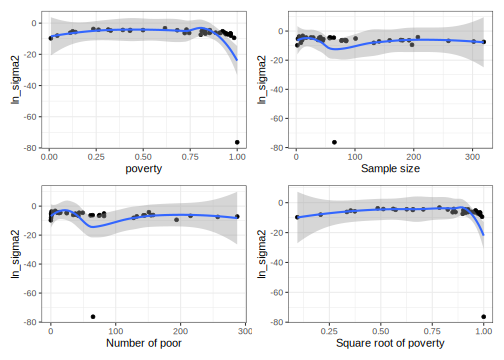
\includegraphics{02_S1_FGV_files/figure-latex/unnamed-chunk-9-1.pdf}

\hypertarget{variance-model}{%
\section{Variance Model}\label{variance-model}}

The code fits a multiple linear regression model (using the \texttt{lm()} function), where \texttt{ln\_sigma2} is the response variable and the predictor variables include \texttt{pobreza}, \texttt{nd}, and various transformations of these variables. The goal of this model is to estimate the generalized variance function (FGV) for the observed domains.

\begin{Shaded}
\begin{Highlighting}[]
\FunctionTok{library}\NormalTok{(gtsummary)}
\NormalTok{FGV1 }\OtherTok{\textless{}{-}} \FunctionTok{lm}\NormalTok{(ln\_sigma2 }\SpecialCharTok{\textasciitilde{}} \SpecialCharTok{{-}}\DecValTok{1} \SpecialCharTok{+}\NormalTok{  pobreza }\SpecialCharTok{+}
             \FunctionTok{I}\NormalTok{(pobreza}\SpecialCharTok{*}\NormalTok{nd),}
     \AttributeTok{data =}\NormalTok{ baseFGV)}

\FunctionTok{tbl\_regression}\NormalTok{(FGV1) }\SpecialCharTok{\%\textgreater{}\%} 
  \FunctionTok{add\_glance\_table}\NormalTok{(}\AttributeTok{include =} \FunctionTok{c}\NormalTok{(r.squared, adj.r.squared))}
\end{Highlighting}
\end{Shaded}

\begin{tabular}{l|c|c|c}
\hline
**Characteristic** & **Beta** & **95\% CI** & **p-value**\\
\hline
pobreza & -12 & -20, -4.5 & 0.003\\
\hline
I(pobreza * nd) & 0.02 & -0.04, 0.07 & 0.5\\
\hline
R² & 0.345 &  & \\
\hline
Adjusted R² & 0.311 &  & \\
\hline
\end{tabular}

After obtaining the model estimation, the value of the constant \(\Delta\) must be obtained, for which the following code is used.

\begin{Shaded}
\begin{Highlighting}[]
\NormalTok{delta.hat }\OtherTok{=} \FunctionTok{sum}\NormalTok{(baseFGV}\SpecialCharTok{$}\NormalTok{vardir) }\SpecialCharTok{/} 
  \FunctionTok{sum}\NormalTok{(}\FunctionTok{exp}\NormalTok{(}\FunctionTok{fitted.values}\NormalTok{(FGV1)))}
\end{Highlighting}
\end{Shaded}

From which it is derived that \(\Delta = 0.110434\). Finally, it is possible to obtain the smoothed variance by executing the following command.

\begin{Shaded}
\begin{Highlighting}[]
\NormalTok{hat.sigma }\OtherTok{\textless{}{-}} 
  \FunctionTok{data.frame}\NormalTok{(}\AttributeTok{dam2 =}\NormalTok{ baseFGV}\SpecialCharTok{$}\NormalTok{dam2,}
             \AttributeTok{hat\_var =}\NormalTok{ delta.hat }\SpecialCharTok{*} \FunctionTok{exp}\NormalTok{(}\FunctionTok{fitted.values}\NormalTok{(FGV1)))}

\NormalTok{baseFGV }\OtherTok{\textless{}{-}} \FunctionTok{left\_join}\NormalTok{(baseFGV, hat.sigma)}
\FunctionTok{tba}\NormalTok{(}\FunctionTok{head}\NormalTok{(baseFGV, }\DecValTok{10}\NormalTok{))}
\end{Highlighting}
\end{Shaded}

\begin{table}[H]
\centering
\centering
\begin{tabular}[t]{lrrrrr}
\toprule
dam2 & pobreza & nd & vardir & ln\_sigma2 & hat\_var\\
\midrule
0102 & 0.9836 & 197 & 0.0001 & -9.4372 & 0e+00\\
0103 & 1.0000 & 65 & 0.0000 & -76.3620 & 0e+00\\
0202 & 0.9391 & 141 & 0.0009 & -7.0701 & 0e+00\\
0203 & 0.8117 & 101 & 0.0060 & -5.1159 & 0e+00\\
0205 & 0.9646 & 85 & 0.0011 & -6.8149 & 0e+00\\
\addlinespace
0212 & 0.8304 & 59 & 0.0101 & -4.5936 & 0e+00\\
0301 & 0.9419 & 45 & 0.0013 & -6.6569 & 0e+00\\
0302 & 0.9109 & 159 & 0.0017 & -6.3681 & 0e+00\\
0401 & 0.8063 & 319 & 0.0006 & -7.4369 & 4e-04\\
0402 & 0.8311 & 259 & 0.0012 & -6.7172 & 1e-04\\
\bottomrule
\end{tabular}
\end{table}

Model validation for the FGV

\begin{Shaded}
\begin{Highlighting}[]
\FunctionTok{par}\NormalTok{(}\AttributeTok{mfrow =} \FunctionTok{c}\NormalTok{(}\DecValTok{2}\NormalTok{, }\DecValTok{2}\NormalTok{))}
\FunctionTok{plot}\NormalTok{(FGV1)}
\end{Highlighting}
\end{Shaded}

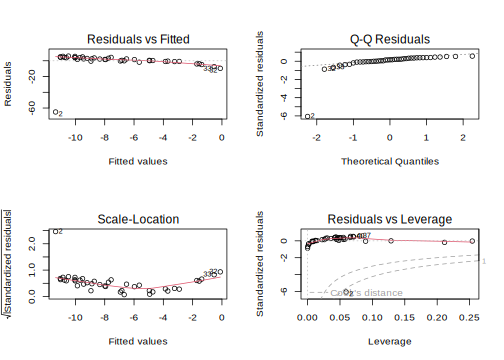
\includegraphics{02_S1_FGV_files/figure-latex/unnamed-chunk-13-1.pdf}

Smoothed variance prediction

\begin{Shaded}
\begin{Highlighting}[]
\NormalTok{base\_sae }\OtherTok{\textless{}{-}} \FunctionTok{left\_join}\NormalTok{(indicador\_dam,}
\NormalTok{                      baseFGV }\SpecialCharTok{\%\textgreater{}\%} \FunctionTok{select}\NormalTok{(id\_dominio, hat\_var),}
                      \AttributeTok{by =}\NormalTok{ id\_dominio) }\SpecialCharTok{\%\textgreater{}\%}
  \FunctionTok{mutate}\NormalTok{(}
    \AttributeTok{pobreza\_var =} \FunctionTok{ifelse}\NormalTok{(}\FunctionTok{is.na}\NormalTok{(hat\_var), }\ConstantTok{NA\_real\_}\NormalTok{, pobreza\_var),}
    \AttributeTok{pobreza\_deff =} \FunctionTok{ifelse}\NormalTok{(}\FunctionTok{is.na}\NormalTok{(hat\_var), }\ConstantTok{NA\_real\_}\NormalTok{, pobreza\_deff)}
\NormalTok{  )}
\end{Highlighting}
\end{Shaded}

Now, we make a line graph to see the volatility and the estimates of the variances.

\begin{Shaded}
\begin{Highlighting}[]
\NormalTok{nDom }\OtherTok{\textless{}{-}} \FunctionTok{sum}\NormalTok{(}\SpecialCharTok{!}\FunctionTok{is.na}\NormalTok{(base\_sae}\SpecialCharTok{$}\NormalTok{hat\_var))}
\NormalTok{temp\_FH }\OtherTok{\textless{}{-}}\NormalTok{ base\_sae }\SpecialCharTok{\%\textgreater{}\%} \FunctionTok{filter}\NormalTok{(}\SpecialCharTok{!}\FunctionTok{is.na}\NormalTok{(hat\_var))}
\FunctionTok{ggplot}\NormalTok{(temp\_FH }\SpecialCharTok{\%\textgreater{}\%}
         \FunctionTok{arrange}\NormalTok{(n\_pobreza), }\FunctionTok{aes}\NormalTok{(}\AttributeTok{x =} \DecValTok{1}\SpecialCharTok{:}\NormalTok{nDom)) }\SpecialCharTok{+}
  \FunctionTok{geom\_line}\NormalTok{(}\FunctionTok{aes}\NormalTok{(}\AttributeTok{y =}\NormalTok{ pobreza\_var, }\AttributeTok{color =} \StringTok{"VarDirEst"}\NormalTok{)) }\SpecialCharTok{+}
  \FunctionTok{geom\_line}\NormalTok{(}\FunctionTok{aes}\NormalTok{(}\AttributeTok{y =}\NormalTok{ hat\_var, }\AttributeTok{color =} \StringTok{"FGV"}\NormalTok{)) }\SpecialCharTok{+}
  \FunctionTok{labs}\NormalTok{(}\AttributeTok{y =} \StringTok{"Varianzas"}\NormalTok{, }\AttributeTok{x =} \StringTok{"Sample size"}\NormalTok{, }\AttributeTok{color =} \StringTok{" "}\NormalTok{) }\SpecialCharTok{+}
  \FunctionTok{scale\_x\_continuous}\NormalTok{(}\AttributeTok{breaks =} \FunctionTok{seq}\NormalTok{(}\DecValTok{1}\NormalTok{, nDom, }\AttributeTok{by =} \DecValTok{10}\NormalTok{),}
\AttributeTok{labels =}\NormalTok{ temp\_FH}\SpecialCharTok{$}\NormalTok{n\_pobreza[}\FunctionTok{order}\NormalTok{(temp\_FH}\SpecialCharTok{$}\NormalTok{n\_pobreza)][}\FunctionTok{seq}\NormalTok{(}\DecValTok{1}\NormalTok{, nDom, }\AttributeTok{by =} \DecValTok{10}\NormalTok{)]) }\SpecialCharTok{+}
  \FunctionTok{scale\_color\_manual}\NormalTok{(}\AttributeTok{values =} \FunctionTok{c}\NormalTok{(}\StringTok{"FGV"} \OtherTok{=} \StringTok{"Blue"}\NormalTok{, }\StringTok{"VarDirEst"} \OtherTok{=} \StringTok{"Red"}\NormalTok{))}
\end{Highlighting}
\end{Shaded}

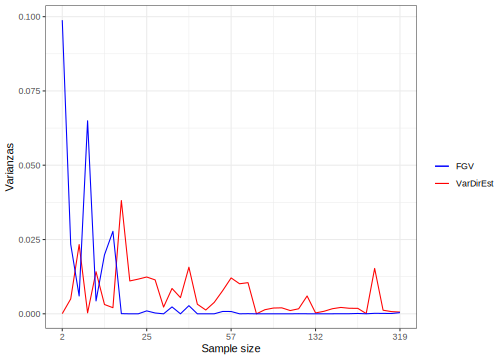
\includegraphics{02_S1_FGV_files/figure-latex/unnamed-chunk-15-1.pdf}

This code performs several transformations on the dataset \texttt{base\_sae}:

\begin{enumerate}
\def\labelenumi{\arabic{enumi}.}
\tightlist
\item
  \textbf{Creation of new variables:}

  \begin{itemize}
  \tightlist
  \item
    \texttt{pobreza\_deff}: Replaces NaN values with 1 if they exist; otherwise, it keeps the original value.
  \item
    \texttt{deff\_FGV}: Computes a new Design Effect (DEFF) using the formula \texttt{hat\_var\ /\ (pobreza\_var\ /\ pobreza\_deff)} when \texttt{pobreza\_var} is not equal to 0.
  \item
    \texttt{n\_eff\_FGV}: Calculates the effective number of surveyed individuals as \texttt{n\_pobreza\ /\ deff\_FGV}.
  \end{itemize}
\item
  \textbf{Modification of the variable \texttt{pobreza}:}

  \begin{itemize}
  \tightlist
  \item
    If \texttt{hat\_var} is NA, it replaces \texttt{pobreza} values with NA; otherwise, it retains the original value.
  \end{itemize}
\end{enumerate}

\begin{Shaded}
\begin{Highlighting}[]
\NormalTok{base\_FH }\OtherTok{\textless{}{-}}\NormalTok{ base\_sae }\SpecialCharTok{\%\textgreater{}\%}
  \FunctionTok{mutate}\NormalTok{(}
    \AttributeTok{pobreza\_deff =} \FunctionTok{ifelse}\NormalTok{(}\FunctionTok{is.nan}\NormalTok{(pobreza\_deff), }\DecValTok{1}\NormalTok{, pobreza\_deff),}
    \AttributeTok{deff\_FGV =} \FunctionTok{ifelse}\NormalTok{(pobreza\_var }\SpecialCharTok{==} \DecValTok{0}\NormalTok{ ,}
      \DecValTok{1}\NormalTok{,}
\NormalTok{      hat\_var }\SpecialCharTok{/}\NormalTok{ (pobreza\_var }\SpecialCharTok{/}\NormalTok{ pobreza\_deff) }\CommentTok{\#Fórmula del nuevo DEFF}
\NormalTok{    ),}
    \CommentTok{\# Criterio MDS para regularizar el DeffFGV}
    \AttributeTok{n\_eff\_FGV =}\NormalTok{ n\_pobreza }\SpecialCharTok{/}\NormalTok{ deff\_FGV, }\CommentTok{\#Número efectivo de personas encuestadas}

     \AttributeTok{pobreza =} \FunctionTok{ifelse}\NormalTok{(}\FunctionTok{is.na}\NormalTok{(hat\_var), }\ConstantTok{NA\_real\_}\NormalTok{, pobreza) }
\NormalTok{  )}


\CommentTok{\#saveRDS(object = base\_FH, "Recursos/02\_FGV/base\_FH\_2020.rds")}
\end{Highlighting}
\end{Shaded}

\hypertarget{session-3--fay-herriot-model---poverty-estimation}{%
\chapter{Session 3- Fay Herriot Model - Poverty Estimation}\label{session-3--fay-herriot-model---poverty-estimation}}

The Fay Herriot model, proposed by Fay and Herriot (1979), is a statistical area model and is the most commonly used. It's essential to note that within small area estimation methodology, area models are the most applied because having individual-level information is often not feasible. Instead, we typically have data at the area level along with associated auxiliary information. This mixed linear model was the first to include random effects at the area level, implying that most of the information fed into the model corresponds to usually aggregated units like departments, regions, provinces, municipalities, among others. The estimates obtained from the model are over these aggregations or subpopulations.

Now, the Fay Herriot model relates area indicators \(\theta_d\), where \(d\) ranges from 1 to \(D\), assuming they vary with respect to a vector of \(p\) covariates \(\boldsymbol{x}_d\). The model is defined by the equation \(\theta_d = \boldsymbol{x}^{T}_{d}\boldsymbol{\beta} + u_d\), where \(u_d\) is the error term or random effect, distinct for each area and distributed as \(u_{d} \stackrel{ind}{\sim}\left(0,\sigma_{u}^{2}\right)\).

However, the true values of the indicators \(\theta_d\) are not observable. Hence, the direct estimator \(\hat{\theta}^{DIR}_d\) is used to estimate them, leading to sampling error. This estimator is still considered unbiased under the sample design, i.e.,
\[
\hat{\theta}_d^{DIR} = \theta_d + e_d  
\]

The model is then fitted using the sampling error term \(e_d\), where \(e_{d} \stackrel{ind}{\sim} \left(0,\sigma^2_{e_d}\right)\), and the variances \(\sigma^2_{e_d}\) are estimated using survey microdata. The FH model is rewritten as

\[
\hat{\theta}^{DIR}_{d} = \boldsymbol{x}^{T}_{d}\boldsymbol{\beta} + u_d + e_d
\].

The best linear unbiased predictor (BLUP) under the FH model is given by

\[
\tilde{\theta}_{d}^{FH} = \boldsymbol{x}^{T}_{d}\tilde{\boldsymbol{\beta}}+\tilde{u}_{d}
\],

where \(\tilde{u}_d = \gamma_d\left(\hat{\theta}^{DIR}_{d} - \boldsymbol{x}^{T}_{d}\tilde{\boldsymbol{\beta}} \right)\) and \(\gamma_d=\frac{\sigma^2_u}{\sigma^2_u + \sigma^2_{e_d}}\).

\hypertarget{area-model-for-poverty-estimation}{%
\subsection*{Area Model for Poverty Estimation}\label{area-model-for-poverty-estimation}}
\addcontentsline{toc}{subsection}{Area Model for Poverty Estimation}

Let \(P_d\) be the probability of finding a person in a state of poverty in the \(d\)-th domain of the population. Then, the direct estimator of \(P_d\) can be written as:

\[
\hat{P}^{DIR}_{d} = P_d + e_d
\]

Now, \(P_d\) can be modeled as follows:

\[
P_d = \boldsymbol{x}^{T}_{d}\boldsymbol{\beta} + u_d
\]

Rewriting \(\hat{P}^{DIR}_{d}\) in terms of the two previous equations, we have:

\[
\hat{P}^{DIR}_{d} = \boldsymbol{x}^{T}_{d}\boldsymbol{\beta} + u_d + e_d
\]

It is then possible to assume that \(\hat{P}^{DIR}_d \sim N(\boldsymbol{x}^{T}_{d}\boldsymbol \beta, \sigma_u^2 +\sigma_{e_d}^2)\), \(\hat{P}^{DIR}_d \mid u_d \sim N(\boldsymbol{x}^{T}_{d}\boldsymbol \beta + u_d,\sigma_{e_d}^2)\), and \(u_d \sim N(0, \sigma^2_u)\).

Next, prior distributions are assumed for \(\boldsymbol{\beta}\) and \(\sigma^2_u\):

\begin{align*}
\beta_p & \sim N(0, 10000)\\
\sigma^2_u &\sim IG(0.0001, 0.0001)
\end{align*}

Therefore, the Bayesian estimator for \(P_d\) is given as \(\tilde{P}_d = E\left(P_d\mid\hat{P}_d^{DIR}\right)\).

\hypertarget{optimal-predictor-of-p_d}{%
\subsection*{\texorpdfstring{Optimal Predictor of \(P_d\)}{Optimal Predictor of P\_d}}\label{optimal-predictor-of-p_d}}
\addcontentsline{toc}{subsection}{Optimal Predictor of \(P_d\)}

The optimal predictor of \(P_d\) is given by:

\[E(P_d | \hat{P}^{DIR}_d) = \gamma_d\hat{P}^{DIR}_d + (1-\gamma_d)\boldsymbol{x}^{T}_{d}\boldsymbol \beta\]

where \(\gamma_d = \frac{\sigma_u^2}{\sigma_u^2 +\sigma_{e_d}^2}\).

We know that \(\hat{P}^{DIR}_d \sim N(\boldsymbol{x}^{T}_{d}\boldsymbol \beta, \sigma_u^2 +\sigma_{e_d}^2)\), \(\hat{P}^{DIR}_d \mid u_d \sim N(\boldsymbol{x}^{T}_{d}\boldsymbol \beta + u_d,\sigma_{e_d}^2)\), and \(u_d \sim N(0, \sigma^2_u)\).

Therefore, the optimal predictor is determined by a weighted combination of the direct estimator \(\hat{P}^{DIR}_d\) and the linear predictor \(\boldsymbol{x}^{T}_{d}\boldsymbol \beta\) where the weights are determined by the ratio of the variance components, providing an optimal balance between the direct estimate and the model-based prediction.

\begin{align*}
f(u_d| \hat{P}^{DIR}_d) \propto f(\hat{P}^{DIR}_d | u_d)f(u_d) & = \frac{1}{\sigma^2_{e_d}\sqrt{2\pi}}\exp\left\{-\frac{1}{2\sigma^2_{e_d}(\hat{P}^{DIR}_d-\boldsymbol{x}^{T}_{d}\boldsymbol \beta - u_d)^2}\right\} \frac{1}{\sigma^2_u\sqrt{2\pi}}\exp\left\{- \frac{1}{2\sigma^2_u}u_d^2\right\}\\
& \propto \exp\left\{-\frac{u_d^2 - 2u_d(\hat{P}^{DIR}_d-\boldsymbol{x}^{T}_{d}\boldsymbol \beta)}{2\sigma^2_{e_d}} - \frac{u_d^2}{2\sigma^2_u}\right\} \\
& = \exp\left\{-\frac{1}{2}\left[(\frac{1}{\sigma^2_{e_d}} + \frac{1}{\sigma^2_u})u_d^2 - 2\frac{\hat{P}^{DIR}_d-\boldsymbol{x}^{T}_{d}\boldsymbol \beta}{\sigma_{e_d}^2}u_d\right] \right\} \\
& = \exp \left\{ -\frac{1}{2\frac{\sigma_u^2\sigma_{e_d}^2}{\sigma_u^2 +\sigma_{e_d}^2}}\left[u_d^2 - 2\frac{\sigma_u^2}{\sigma_u^2 +\sigma_{e_d}^2}(\hat{P}^{DIR}_d-\boldsymbol{x}^{T}_{d}\boldsymbol \beta)u_d \right] \right\} \\
& \propto \exp \left\{ -\frac{1}{2\frac{\sigma_u^2\sigma_{e_d}^2}{\sigma_u^2 +\sigma_{e_d}^2}}\left[u_d -  \frac{\sigma_u^2}{\sigma_u^2 +\sigma_{e_d}^2}(\hat{P}^{DIR}_d-\boldsymbol{x}^{T}_{d}\boldsymbol \beta)\right]^2 \right\} \\
& \propto N(E(u_d|\hat{P}^{DIR}_d), \text{Var}(u_d|P^{DIR}))
\end{align*}

with \(E(u_d|\hat{P}^{DIR}_d) = \frac{\sigma_u^2}{\sigma_u^2 +\sigma_{e_d}^2}(\hat{P}^{DIR}_d-\boldsymbol{x}^{T}_{d}\boldsymbol \beta)\) y \(\text{Var}(u_d|P^{DIR}) = \frac{\sigma_u^2\sigma_{e_d}^2}{\sigma_u^2 +\sigma_{e_d}^2}\). Therefore you have,

\begin{align*}
E(P_d | \hat{P}^{DIR}_d) = \boldsymbol{x}^{T}_{d}\boldsymbol \beta + E(u_d|\hat{P}^{DIR}_d) & =  \boldsymbol{x}^{T}_{d}\boldsymbol \beta + \frac{\sigma_u^2}{\sigma_u^2 +\sigma_{e_d}^2}(\hat{P}^{DIR}_d-\boldsymbol{x}^{T}_{d}\boldsymbol \beta) \\
& = \frac{\sigma_{e_d}^2}{\sigma_u^2 +\sigma_{e_d}^2}\hat{P}^{DIR}_d + \frac{\sigma_u^2}{\sigma_u^2 +\sigma_{e_d}^2}\boldsymbol{x}^{T}_{d}\boldsymbol \beta \\
& = \gamma_d\hat{P}^{DIR}_d + (1-\gamma_d)\boldsymbol{x}^{T}_{d}\boldsymbol \beta
\end{align*}

\hypertarget{estimation-procedure}{%
\section{Estimation Procedure}\label{estimation-procedure}}

This code utilizes the libraries \texttt{tidyverse} and \texttt{magrittr} for data processing and analysis.

The function \texttt{readRDS()} is used to load a data file in RDS format, containing direct estimates and smoothed variance for the proportion of individuals in poverty for the year 2018. Subsequently, the \texttt{\%\textgreater{}\%} operator from the \texttt{magrittr} library is employed to chain the selection of specific columns, namely \texttt{dam2}, \texttt{nd}, \texttt{pobreza}, \texttt{vardir}, and \texttt{hat\_var}.

\begin{Shaded}
\begin{Highlighting}[]
\FunctionTok{library}\NormalTok{(tidyverse)}
\FunctionTok{library}\NormalTok{(magrittr)}
\NormalTok{base\_FH }\OtherTok{\textless{}{-}} \FunctionTok{readRDS}\NormalTok{(}\StringTok{"Recursos/03\_FH\_normal/01\_base\_FH.Rds"}\NormalTok{) }\SpecialCharTok{\%\textgreater{}\%} 
  \FunctionTok{select}\NormalTok{(dam2,pobreza,hat\_var)}
\end{Highlighting}
\end{Shaded}

Reading the covariates, which have been previously obtained. Due to the difference in scales between variables, an adjustment is necessary.

\begin{Shaded}
\begin{Highlighting}[]
\NormalTok{statelevel\_predictors\_df }\OtherTok{\textless{}{-}}
  \FunctionTok{readRDS}\NormalTok{(}\StringTok{\textquotesingle{}Recursos/03\_FH\_normal/02\_statelevel\_predictors\_dam.rds\textquotesingle{}}\NormalTok{) }\SpecialCharTok{\%\textgreater{}\%} 
  \FunctionTok{mutate}\NormalTok{(}\AttributeTok{id\_order =} \DecValTok{1}\SpecialCharTok{:}\FunctionTok{n}\NormalTok{())}
\end{Highlighting}
\end{Shaded}

Next, a full join (\texttt{full\_join}) is performed between the dataset \texttt{base\_FH} and the predictors \texttt{statelevel\_predictors\_df} using the variable \texttt{dam2} as the joining key.

The function \texttt{tba()} is used to display the first 10 rows and 8 columns of the resulting dataset from the previous join.

A full join (\texttt{full\_join}) combines data from both datasets, preserving all rows from both and filling in missing values (NA) if matches aren't found based on the joining variable (dam2 in this case).

The \texttt{tba()} function displays an HTML-formatted table in the R console showing the first 10 rows and 8 columns of the resulting dataset from the join.

\begin{Shaded}
\begin{Highlighting}[]
\NormalTok{base\_FH }\OtherTok{\textless{}{-}} \FunctionTok{full\_join}\NormalTok{(base\_FH, statelevel\_predictors\_df, }\AttributeTok{by =} \StringTok{"dam2"}\NormalTok{ )}
\FunctionTok{tba}\NormalTok{(base\_FH[}\DecValTok{1}\SpecialCharTok{:}\DecValTok{10}\NormalTok{,}\DecValTok{1}\SpecialCharTok{:}\DecValTok{8}\NormalTok{])}
\end{Highlighting}
\end{Shaded}

\begin{table}[H]
\centering
\centering
\begin{tabular}[t]{lrrrrrrr}
\toprule
dam2 & pobreza & hat\_var & area1 & sex2 & age2 & age3 & age4\\
\midrule
0101 & NA & NA & 1.0000 & 0.5087 & 0.2694 & 0.2297 & 0.1689\\
0102 & 0.9836 & 0 & 1.0000 & 0.4754 & 0.2857 & 0.2261 & 0.1527\\
0103 & 1.0000 & 0 & 1.0000 & 0.5037 & 0.3095 & 0.2015 & 0.1312\\
0201 & NA & NA & 0.5147 & 0.5060 & 0.2962 & 0.2090 & 0.1844\\
0202 & 0.9391 & 0 & 0.9986 & 0.5376 & 0.2625 & 0.2226 & 0.2238\\
\addlinespace
0203 & 0.8117 & 0 & 0.9754 & 0.5432 & 0.2454 & 0.2254 & 0.2388\\
0204 & NA & NA & 1.0000 & 0.5300 & 0.3151 & 0.2022 & 0.2034\\
0205 & 0.9646 & 0 & 1.0000 & 0.5182 & 0.3057 & 0.2286 & 0.1981\\
0206 & NA & NA & 1.0000 & 0.5157 & 0.3192 & 0.1959 & 0.1552\\
0207 & NA & NA & 1.0000 & 0.5097 & 0.3099 & 0.1966 & 0.1691\\
\bottomrule
\end{tabular}
\end{table}

\begin{Shaded}
\begin{Highlighting}[]
\CommentTok{\# View(base\_FH)}
\end{Highlighting}
\end{Shaded}

\hypertarget{preparing-the-supplies-for-stan}{%
\section{\texorpdfstring{Preparing the supplies for \texttt{STAN}}{Preparing the supplies for STAN}}\label{preparing-the-supplies-for-stan}}

\begin{enumerate}
\def\labelenumi{\arabic{enumi}.}
\item
  Splitting the database into observed and unobserved domains.

  Observed domains.
\end{enumerate}

\begin{Shaded}
\begin{Highlighting}[]
\NormalTok{data\_dir }\OtherTok{\textless{}{-}}\NormalTok{ base\_FH }\SpecialCharTok{\%\textgreater{}\%} \FunctionTok{filter}\NormalTok{(}\SpecialCharTok{!}\FunctionTok{is.na}\NormalTok{(pobreza))}
\end{Highlighting}
\end{Shaded}

Unobserved domains.

\begin{Shaded}
\begin{Highlighting}[]
\NormalTok{data\_syn }\OtherTok{\textless{}{-}}
\NormalTok{  base\_FH }\SpecialCharTok{\%\textgreater{}\%} \FunctionTok{anti\_join}\NormalTok{(data\_dir }\SpecialCharTok{\%\textgreater{}\%} \FunctionTok{select}\NormalTok{(dam2))}
\FunctionTok{tba}\NormalTok{(data\_syn[}\DecValTok{1}\SpecialCharTok{:}\DecValTok{10}\NormalTok{, }\DecValTok{1}\SpecialCharTok{:}\DecValTok{8}\NormalTok{])}
\end{Highlighting}
\end{Shaded}

\begin{table}[H]
\centering
\centering
\begin{tabular}[t]{lrrrrrrr}
\toprule
dam2 & pobreza & hat\_var & area1 & sex2 & age2 & age3 & age4\\
\midrule
0101 & NA & NA & 1.0000 & 0.5087 & 0.2694 & 0.2297 & 0.1689\\
0201 & NA & NA & 0.5147 & 0.5060 & 0.2962 & 0.2090 & 0.1844\\
0204 & NA & NA & 1.0000 & 0.5300 & 0.3151 & 0.2022 & 0.2034\\
0206 & NA & NA & 1.0000 & 0.5157 & 0.3192 & 0.1959 & 0.1552\\
0207 & NA & NA & 1.0000 & 0.5097 & 0.3099 & 0.1966 & 0.1691\\
\addlinespace
0208 & NA & NA & 1.0000 & 0.5256 & 0.2880 & 0.2218 & 0.1974\\
0209 & NA & NA & 1.0000 & 0.5149 & 0.3018 & 0.2100 & 0.1759\\
0210 & NA & NA & 0.9779 & 0.5194 & 0.3000 & 0.2111 & 0.1828\\
0211 & NA & NA & 1.0000 & 0.5427 & 0.2645 & 0.2192 & 0.2267\\
0502 & NA & NA & 0.3699 & 0.4974 & 0.2727 & 0.1824 & 0.1795\\
\bottomrule
\end{tabular}
\end{table}

\begin{enumerate}
\def\labelenumi{\arabic{enumi}.}
\setcounter{enumi}{1}
\item
  Defining the fixed-effects matrix.

  Defines a linear model using the \texttt{formula()} function, incorporating various predictor variables such as age, ethnicity, unemployment rate, among others.

  Utilizes the \texttt{model.matrix()} function to generate design matrices (\texttt{Xdat} and \texttt{Xs}) from the observed (\texttt{data\_observed}) and unobserved (\texttt{data\_unobserved}) data to use in building regression models. The \texttt{model.matrix()} function transforms categorical variables into binary (dummy) variables, allowing them to be used in modeling.
\end{enumerate}

\begin{Shaded}
\begin{Highlighting}[]
\NormalTok{formula\_mod  }\OtherTok{\textless{}{-}} \FunctionTok{formula}\NormalTok{(}\SpecialCharTok{\textasciitilde{}}\NormalTok{  ODDJOB }\SpecialCharTok{+}\NormalTok{ WORKED }\SpecialCharTok{+}
\NormalTok{                         stable\_lights\_mean }\SpecialCharTok{+} 
\NormalTok{                         accessibility\_mean }\SpecialCharTok{+} 
\NormalTok{                         urban.coverfraction\_sum)}
\DocumentationTok{\#\# Dominios observados}
\NormalTok{Xdat }\OtherTok{\textless{}{-}} \FunctionTok{model.matrix}\NormalTok{(formula\_mod, }\AttributeTok{data =}\NormalTok{ data\_dir)}

\DocumentationTok{\#\# Dominios no observados}
\NormalTok{Xs }\OtherTok{\textless{}{-}} \FunctionTok{model.matrix}\NormalTok{(formula\_mod, }\AttributeTok{data =}\NormalTok{ data\_syn)}
\FunctionTok{dim}\NormalTok{(Xs)}
\end{Highlighting}
\end{Shaded}

\begin{verbatim}
## [1] 22  6
\end{verbatim}

\begin{Shaded}
\begin{Highlighting}[]
\FunctionTok{dim}\NormalTok{(data\_syn)}
\end{Highlighting}
\end{Shaded}

\begin{verbatim}
## [1] 22 33
\end{verbatim}

\begin{enumerate}
\def\labelenumi{\arabic{enumi}.}
\setcounter{enumi}{2}
\tightlist
\item
  Creando lista de parámetros para \texttt{STAN}
\end{enumerate}

\begin{Shaded}
\begin{Highlighting}[]
\NormalTok{sample\_data }\OtherTok{\textless{}{-}} \FunctionTok{list}\NormalTok{(}
  \AttributeTok{N1 =} \FunctionTok{nrow}\NormalTok{(Xdat),   }\CommentTok{\# Observed.}
  \AttributeTok{N2 =} \FunctionTok{nrow}\NormalTok{(Xs),   }\CommentTok{\# Not observed.}
  \AttributeTok{p  =} \FunctionTok{ncol}\NormalTok{(Xdat),       }\CommentTok{\# Number of predictors.}
  \AttributeTok{X  =} \FunctionTok{as.matrix}\NormalTok{(Xdat),  }\CommentTok{\# Observed covariates.}
  \AttributeTok{Xs =} \FunctionTok{as.matrix}\NormalTok{(Xs),    }\CommentTok{\# Not observed covariates.}
  \AttributeTok{y  =} \FunctionTok{as.numeric}\NormalTok{(data\_dir}\SpecialCharTok{$}\NormalTok{pobreza), }\CommentTok{\# Direct estimation}
  \AttributeTok{sigma\_e =} \FunctionTok{sqrt}\NormalTok{(data\_dir}\SpecialCharTok{$}\NormalTok{hat\_var)   }\CommentTok{\# Estimation error}
\NormalTok{)}
\end{Highlighting}
\end{Shaded}

Rutina implementada en \texttt{STAN}

\begin{verbatim}
data {
  int<lower=0> N1;   // number of data items
  int<lower=0> N2;   // number of data items for prediction
  int<lower=0> p;   // number of predictors
  matrix[N1, p] X;   // predictor matrix
  matrix[N2, p] Xs;   // predictor matrix
  vector[N1] y;      // predictor matrix 
  vector[N1] sigma_e; // known variances
}

parameters {
  vector[p] beta;       // coefficients for predictors
  real<lower=0> sigma2_u;
  vector[N1] u;
}

transformed parameters{
  vector[N1] theta;
  vector[N1] thetaSyn;
  vector[N1] thetaFH;
  vector[N1] gammaj;
  real<lower=0> sigma_u;
  thetaSyn = X * beta;
  theta = thetaSyn + u;
  sigma_u = sqrt(sigma2_u);
  gammaj =  to_vector(sigma_u ./ (sigma_u + sigma_e));
  thetaFH = (gammaj) .* y + (1-gammaj).*thetaSyn; 
}

model {
  // likelihood
  y ~ normal(theta, sigma_e); 
  // priors
  beta ~ normal(0, 100);
  u ~ normal(0, sigma_u);
  sigma2_u ~ inv_gamma(0.0001, 0.0001);
}

generated quantities{
  vector[N2] y_pred;
  for(j in 1:N2) {
    y_pred[j] = normal_rng(Xs[j] * beta, sigma_u);
  }
}
\end{verbatim}

\begin{enumerate}
\def\labelenumi{\arabic{enumi}.}
\setcounter{enumi}{3}
\tightlist
\item
  Compiling the model in \texttt{STAN}.
  Here's the process to compile the \texttt{STAN} code from R:
\end{enumerate}

This code utilizes the \texttt{rstan} library to fit a Bayesian model using the file \texttt{17FH\_normal.stan}, which contains the model written in the Stan probabilistic modeling language.

Initially, the \texttt{stan()} function is employed to fit the model to the \texttt{sample\_data}. The arguments passed to \texttt{stan()} include the file containing the model (\texttt{fit\_FH\_normal}), the data (\texttt{sample\_data}), and control arguments for managing the model fitting process, such as the number of iterations for the warmup period (\texttt{warmup}), the sampling period (\texttt{iter}), and the number of CPU cores to use for the fitting process (\texttt{cores}).

Additionally, the \texttt{parallel::detectCores()} function is used to automatically detect the number of available CPU cores. The \texttt{mc.cores} option is then set to utilize the maximum number of available cores for the model fitting.

The outcome of the model fitting is stored in \texttt{model\_FH\_normal}, which contains a sample from the posterior distribution of the model. This sample can be employed for inferences about the model parameters and predictions. Overall, this code is useful for fitting Bayesian models using Stan and conducting subsequent inferences.

\begin{Shaded}
\begin{Highlighting}[]
\FunctionTok{library}\NormalTok{(rstan)}
\NormalTok{fit\_FH\_normal }\OtherTok{\textless{}{-}} \StringTok{"Recursos/03\_FH\_normal/modelosStan/17FH\_normal.stan"}
\FunctionTok{options}\NormalTok{(}\AttributeTok{mc.cores =}\NormalTok{ parallel}\SpecialCharTok{::}\FunctionTok{detectCores}\NormalTok{())}
\NormalTok{rstan}\SpecialCharTok{::}\FunctionTok{rstan\_options}\NormalTok{(}\AttributeTok{auto\_write =} \ConstantTok{TRUE}\NormalTok{) }\CommentTok{\# speed up running time }
\NormalTok{model\_FH\_normal }\OtherTok{\textless{}{-}} \FunctionTok{stan}\NormalTok{(}
  \AttributeTok{file =}\NormalTok{ fit\_FH\_normal,  }
  \AttributeTok{data =}\NormalTok{ sample\_data,   }
  \AttributeTok{verbose =} \ConstantTok{FALSE}\NormalTok{,}
  \AttributeTok{warmup =} \DecValTok{2500}\NormalTok{,         }
  \AttributeTok{iter =} \DecValTok{3000}\NormalTok{,            }
  \AttributeTok{cores =} \DecValTok{4}              
\NormalTok{)}
\FunctionTok{saveRDS}\NormalTok{(}\AttributeTok{object =}\NormalTok{ model\_FH\_normal,}
        \AttributeTok{file =} \StringTok{"Recursos/03\_FH\_normal/03\_model\_FH\_normal.rds"}\NormalTok{)}
\end{Highlighting}
\end{Shaded}

Leer el modelo

\begin{Shaded}
\begin{Highlighting}[]
\NormalTok{model\_FH\_normal}\OtherTok{\textless{}{-}} \FunctionTok{readRDS}\NormalTok{(}\StringTok{"Recursos/03\_FH\_normal/03\_model\_FH\_normal.rds"}\NormalTok{)}
\end{Highlighting}
\end{Shaded}

\hypertarget{results-of-the-model-for-observed-domains.}{%
\subsection{Results of the model for observed domains.}\label{results-of-the-model-for-observed-domains.}}

In this code, the \texttt{bayesplot}, \texttt{posterior}, and \texttt{patchwork} libraries are loaded to create graphics and visualizations of the model results.

Subsequently, the \texttt{as.array()} and \texttt{as\_draws\_matrix()} functions are used to extract samples from the posterior distribution of the parameter \texttt{theta} from the model. Then, 100 rows of these samples are randomly selected using the \texttt{sample()} function, resulting in the \texttt{y\_pred2} matrix.

Finally, the \texttt{ppc\_dens\_overlay()} function from \texttt{bayesplot} is utilized to plot a comparison between the empirical distribution of the observed variable \texttt{pobreza} in the data (\texttt{data\_dir\$pobreza}) and the simulated posterior predictive distributions for the same variable (\texttt{y\_pred2}). The \texttt{ppc\_dens\_overlay()} function generates a density plot for both distributions, facilitating the visualization of their comparison.

\begin{Shaded}
\begin{Highlighting}[]
\FunctionTok{library}\NormalTok{(bayesplot)}
\FunctionTok{library}\NormalTok{(posterior)}
\FunctionTok{library}\NormalTok{(patchwork)}
\NormalTok{y\_pred\_B }\OtherTok{\textless{}{-}} \FunctionTok{as.array}\NormalTok{(model\_FH\_normal, }\AttributeTok{pars =} \StringTok{"theta"}\NormalTok{) }\SpecialCharTok{\%\textgreater{}\%} 
  \FunctionTok{as\_draws\_matrix}\NormalTok{()}
\NormalTok{rowsrandom }\OtherTok{\textless{}{-}} \FunctionTok{sample}\NormalTok{(}\FunctionTok{nrow}\NormalTok{(y\_pred\_B), }\DecValTok{100}\NormalTok{)}
\NormalTok{y\_pred2 }\OtherTok{\textless{}{-}}\NormalTok{ y\_pred\_B[rowsrandom, ]}
\NormalTok{p1 }\OtherTok{\textless{}{-}}  \FunctionTok{ppc\_dens\_overlay}\NormalTok{(}\AttributeTok{y =} \FunctionTok{as.numeric}\NormalTok{(data\_dir}\SpecialCharTok{$}\NormalTok{pobreza), y\_pred2)}

\CommentTok{\# ggsave(plot = p1,}
\CommentTok{\#        filename = "Recursos/Día2/Sesion1/0Recursos/FH1.png",}
\CommentTok{\#        scale = 2)}
\NormalTok{p1 }\SpecialCharTok{+} \FunctionTok{geom\_vline}\NormalTok{(}\AttributeTok{xintercept =} \DecValTok{0}\NormalTok{, }\AttributeTok{color =} \StringTok{"red"}\NormalTok{)}
\end{Highlighting}
\end{Shaded}

\includegraphics{Recursos/03_FH_normal/04_ppc_normal.png}

{\textbf{The results indicate that using the Fay-Herriot normal method is not possible, as we are obtaining outcomes outside the boundaries.}}

\hypertarget{area-models---arcsin-transformation.}{%
\section{Area models - ArcSin transformation.}\label{area-models---arcsin-transformation.}}

In its most basic conception, the \textbf{Fay-Herriot} model is a linear combination of covariates. However, the result of this combination can take values that fall outside the acceptable range for a proportion; that is, generally, the Fay-Herriot estimator \(\theta \in \mathbb{R}\), whereas the direct estimator \(\theta \in (0,1)\). The arcsine transformation is given by:

\[
\hat{z}_d = \arcsin\left( \sqrt{ \hat{\theta}_d} \right)
\]

where

\[
Var\left( \hat{z}_d \right) = \frac{\widehat{DEFF}_d}{4\times n_d} = \frac{1}{4\times n_{d, \text{effective}} }
\]

The Fay-Herriot model is defined as follows:

\begin{align*}
Z_d \mid \mu_d,\sigma^2_d &  \sim  N(\mu_d, \sigma^2_d)\\
\mu_d & = \boldsymbol{x}^{T}_{d}\boldsymbol{\beta} + u_d \\
\theta_d & =  \left(\sin(\mu_d)\right)^2
\end{align*}

where \(u_d \sim N(0 , \sigma^2)\).

Let the prior distributions for \(\boldsymbol{\beta}\) and \(\sigma_{u}^{2}\) be given by:

\begin{align*}
\boldsymbol{\beta}  \sim    N\left(0,1000 \right)\\
\sigma_{u}^{2}  \sim    \text{IG}\left(0.0001,0.0001\right)
\end{align*}

\hypertarget{estimation-procedure-1}{%
\subsection{Estimation procedure}\label{estimation-procedure-1}}

Reading the database that resulted in the previous step and selecting the columns of interest

\begin{Shaded}
\begin{Highlighting}[]
\FunctionTok{library}\NormalTok{(tidyverse)}
\FunctionTok{library}\NormalTok{(magrittr)}

\NormalTok{base\_FH }\OtherTok{\textless{}{-}} \FunctionTok{readRDS}\NormalTok{(}\StringTok{\textquotesingle{}Recursos/04\_FH\_Arcosin/01\_base\_FH.Rds\textquotesingle{}}\NormalTok{) }\SpecialCharTok{\%\textgreater{}\%} 
\FunctionTok{transmute}\NormalTok{(dam2,                            }\DocumentationTok{\#\# id dominios}
\NormalTok{          pobreza,}
          \AttributeTok{T\_pobreza =} \FunctionTok{asin}\NormalTok{(}\FunctionTok{sqrt}\NormalTok{(pobreza)),  }\DocumentationTok{\#\# creando zd}
          \AttributeTok{n\_effec =}\NormalTok{ n\_eff\_FGV,              }\DocumentationTok{\#\# n efectivo}
          \AttributeTok{varhat =} \DecValTok{1}\SpecialCharTok{/}\NormalTok{(}\DecValTok{4}\SpecialCharTok{*}\NormalTok{n\_effec)            }\DocumentationTok{\#\# varianza para zd}
\NormalTok{)}
\end{Highlighting}
\end{Shaded}

Joining the two databases.

\begin{Shaded}
\begin{Highlighting}[]
\NormalTok{statelevel\_predictors\_df }\OtherTok{\textless{}{-}}
  \FunctionTok{readRDS}\NormalTok{(}\StringTok{\textquotesingle{}Recursos/03\_FH\_normal/02\_statelevel\_predictors\_dam.rds\textquotesingle{}}\NormalTok{) }\SpecialCharTok{\%\textgreater{}\%}
  \FunctionTok{mutate}\NormalTok{(}\AttributeTok{id\_order =} \DecValTok{1}\SpecialCharTok{:}\FunctionTok{n}\NormalTok{())}
\NormalTok{base\_FH }\OtherTok{\textless{}{-}}
  \FunctionTok{full\_join}\NormalTok{(base\_FH, statelevel\_predictors\_df, }\AttributeTok{by =} \StringTok{"dam2"}\NormalTok{)}
\FunctionTok{tba}\NormalTok{(base\_FH[, }\DecValTok{1}\SpecialCharTok{:}\DecValTok{8}\NormalTok{] }\SpecialCharTok{\%\textgreater{}\%} \FunctionTok{head}\NormalTok{(}\DecValTok{10}\NormalTok{))}
\end{Highlighting}
\end{Shaded}

\begin{table}[H]
\centering
\centering
\begin{tabular}[t]{lrrrrrrr}
\toprule
dam2 & pobreza & T\_pobreza & n\_effec & varhat & area1 & sex2 & age2\\
\midrule
0101 & NA & NA & NA & NA & 1.0000 & 0.5087 & 0.2694\\
0102 & 0.9836 & 1.4422 & 1029.570 & 2.000000e-04 & 1.0000 & 0.4754 & 0.2857\\
0103 & 1.0000 & 1.5708 & 0.000 & 2.226882e+57 & 1.0000 & 0.5037 & 0.3095\\
0201 & NA & NA & NA & NA & 0.5147 & 0.5060 & 0.2962\\
0202 & 0.9391 & 1.3215 & 5881.354 & 0.000000e+00 & 0.9986 & 0.5376 & 0.2625\\
\addlinespace
0203 & 0.8117 & 1.1219 & 6965.029 & 0.000000e+00 & 0.9754 & 0.5432 & 0.2454\\
0204 & NA & NA & NA & NA & 1.0000 & 0.5300 & 0.3151\\
0205 & 0.9646 & 1.3814 & 11790.358 & 0.000000e+00 & 1.0000 & 0.5182 & 0.3057\\
0206 & NA & NA & NA & NA & 1.0000 & 0.5157 & 0.3192\\
0207 & NA & NA & NA & NA & 1.0000 & 0.5097 & 0.3099\\
\bottomrule
\end{tabular}
\end{table}

Selecting the covariates for the model.

\begin{Shaded}
\begin{Highlighting}[]
\NormalTok{names\_cov }\OtherTok{\textless{}{-}}
    \FunctionTok{c}\NormalTok{(}
       \StringTok{"ODDJOB"}\NormalTok{,}\StringTok{"WORKED"}\NormalTok{,}
      \StringTok{"stable\_lights\_mean"}\NormalTok{,}
      \StringTok{"accessibility\_mean"}\NormalTok{,}
      \StringTok{"urban.coverfraction\_sum"}
\NormalTok{    )}
\end{Highlighting}
\end{Shaded}

\hypertarget{preparing-inputs-for-stan}{%
\subsection{\texorpdfstring{Preparing Inputs for \texttt{STAN}}{Preparing Inputs for STAN}}\label{preparing-inputs-for-stan}}

\begin{enumerate}
\def\labelenumi{\arabic{enumi}.}
\tightlist
\item
  Splitting the database into observed and unobserved domains
\end{enumerate}

Observed domains.

\begin{Shaded}
\begin{Highlighting}[]
\NormalTok{data\_dir }\OtherTok{\textless{}{-}}\NormalTok{ base\_FH }\SpecialCharTok{\%\textgreater{}\%} \FunctionTok{filter}\NormalTok{(}\SpecialCharTok{!}\FunctionTok{is.na}\NormalTok{(T\_pobreza))}
\end{Highlighting}
\end{Shaded}

Unobserved domains.

\begin{Shaded}
\begin{Highlighting}[]
\NormalTok{data\_syn }\OtherTok{\textless{}{-}}
\NormalTok{  base\_FH }\SpecialCharTok{\%\textgreater{}\%} \FunctionTok{anti\_join}\NormalTok{(data\_dir }\SpecialCharTok{\%\textgreater{}\%} \FunctionTok{select}\NormalTok{(dam2))}
\end{Highlighting}
\end{Shaded}

\begin{enumerate}
\def\labelenumi{\arabic{enumi}.}
\setcounter{enumi}{1}
\tightlist
\item
  Defining the fixed-effects matrix.
\end{enumerate}

\begin{Shaded}
\begin{Highlighting}[]
\DocumentationTok{\#\# Observed domains}
\NormalTok{Xdat }\OtherTok{\textless{}{-}} \FunctionTok{cbind}\NormalTok{(}\AttributeTok{inter =} \DecValTok{1}\NormalTok{,data\_dir[,names\_cov])}

\DocumentationTok{\#\# Unobserved domains}
\NormalTok{Xs }\OtherTok{\textless{}{-}}  \FunctionTok{cbind}\NormalTok{(}\AttributeTok{inter =} \DecValTok{1}\NormalTok{,data\_syn[,names\_cov])}
\end{Highlighting}
\end{Shaded}

\begin{enumerate}
\def\labelenumi{\arabic{enumi}.}
\setcounter{enumi}{2}
\tightlist
\item
  Creating a parameter list for \texttt{STAN}.
\end{enumerate}

\begin{Shaded}
\begin{Highlighting}[]
\NormalTok{sample\_data }\OtherTok{\textless{}{-}} \FunctionTok{list}\NormalTok{(}
  \AttributeTok{N1 =} \FunctionTok{nrow}\NormalTok{(Xdat),       }\CommentTok{\# Observed.}
  \AttributeTok{N2 =} \FunctionTok{nrow}\NormalTok{(Xs),         }\CommentTok{\# Unobserved.}
  \AttributeTok{p  =} \FunctionTok{ncol}\NormalTok{(Xdat),       }\CommentTok{\# Number of regressors.}
  \AttributeTok{X  =} \FunctionTok{as.matrix}\NormalTok{(Xdat),  }\CommentTok{\# Observed Covariates.}
  \AttributeTok{Xs =} \FunctionTok{as.matrix}\NormalTok{(Xs),    }\CommentTok{\# Unobserved Covariates}
  \AttributeTok{y  =} \FunctionTok{as.numeric}\NormalTok{(data\_dir}\SpecialCharTok{$}\NormalTok{T\_pobreza),}
  \AttributeTok{sigma\_e =} \FunctionTok{sqrt}\NormalTok{(data\_dir}\SpecialCharTok{$}\NormalTok{varhat)}
\NormalTok{)}
\end{Highlighting}
\end{Shaded}

\begin{enumerate}
\def\labelenumi{\arabic{enumi}.}
\setcounter{enumi}{3}
\tightlist
\item
  Compiling the model in \texttt{STAN}.
\end{enumerate}

\begin{Shaded}
\begin{Highlighting}[]
\FunctionTok{library}\NormalTok{(rstan)}
\NormalTok{fit\_FH\_arcoseno }\OtherTok{\textless{}{-}} \StringTok{"Recursos/04\_FH\_Arcosin/modelosStan/15FH\_arcsin\_normal.stan"}
\FunctionTok{options}\NormalTok{(}\AttributeTok{mc.cores =}\NormalTok{ parallel}\SpecialCharTok{::}\FunctionTok{detectCores}\NormalTok{())}
\NormalTok{rstan}\SpecialCharTok{::}\FunctionTok{rstan\_options}\NormalTok{(}\AttributeTok{auto\_write =} \ConstantTok{TRUE}\NormalTok{) }\CommentTok{\# speed up running time }
\NormalTok{model\_FH\_arcoseno }\OtherTok{\textless{}{-}} \FunctionTok{stan}\NormalTok{(}
  \AttributeTok{file =}\NormalTok{ fit\_FH\_arcoseno,  }
  \AttributeTok{data =}\NormalTok{ sample\_data,   }
  \AttributeTok{verbose =} \ConstantTok{FALSE}\NormalTok{,}
  \AttributeTok{warmup =} \DecValTok{2500}\NormalTok{,         }
  \AttributeTok{iter =} \DecValTok{3000}\NormalTok{,            }
  \AttributeTok{cores =} \DecValTok{4}              
\NormalTok{)}
\FunctionTok{saveRDS}\NormalTok{(model\_FH\_arcoseno,}
        \StringTok{"Recursos/04\_FH\_Arcosin/02\_model\_FH\_arcoseno.rds"}\NormalTok{)}
\end{Highlighting}
\end{Shaded}

\begin{Shaded}
\begin{Highlighting}[]
\NormalTok{model\_FH\_arcoseno }\OtherTok{\textless{}{-}} \FunctionTok{readRDS}\NormalTok{(}\StringTok{"Recursos/04\_FH\_Arcosin/02\_model\_FH\_arcoseno.rds"}\NormalTok{)}
\end{Highlighting}
\end{Shaded}

\hypertarget{model-results-for-the-observed-domains.}{%
\subsubsection{Model results for the observed domains.}\label{model-results-for-the-observed-domains.}}

\begin{Shaded}
\begin{Highlighting}[]
\FunctionTok{library}\NormalTok{(bayesplot)}
\FunctionTok{library}\NormalTok{(patchwork)}
\FunctionTok{library}\NormalTok{(posterior)}

\NormalTok{y\_pred\_B }\OtherTok{\textless{}{-}} \FunctionTok{as.array}\NormalTok{(model\_FH\_arcoseno, }\AttributeTok{pars =} \StringTok{"theta"}\NormalTok{) }\SpecialCharTok{\%\textgreater{}\%} 
  \FunctionTok{as\_draws\_matrix}\NormalTok{()}
\NormalTok{rowsrandom }\OtherTok{\textless{}{-}} \FunctionTok{sample}\NormalTok{(}\FunctionTok{nrow}\NormalTok{(y\_pred\_B), }\DecValTok{100}\NormalTok{)}

\NormalTok{y\_pred2 }\OtherTok{\textless{}{-}}\NormalTok{ y\_pred\_B[rowsrandom, ]}
\FunctionTok{ppc\_dens\_overlay}\NormalTok{(}\AttributeTok{y =} \FunctionTok{as.numeric}\NormalTok{(data\_dir}\SpecialCharTok{$}\NormalTok{pobreza), y\_pred2)}
\end{Highlighting}
\end{Shaded}

\begin{figure}
\centering
\includegraphics{Recursos/04_FH_Arcosin/03_ppc_Arcosin.png}
\caption{ppc arcosin}
\end{figure}

Graphical analysis of the convergence of \(\sigma^2_u\) chains.

\begin{Shaded}
\begin{Highlighting}[]
\NormalTok{posterior\_sigma2\_u }\OtherTok{\textless{}{-}} \FunctionTok{as.array}\NormalTok{(model\_FH\_arcoseno, }\AttributeTok{pars =} \StringTok{"sigma2\_u"}\NormalTok{)}
\NormalTok{(}\FunctionTok{mcmc\_dens\_chains}\NormalTok{(posterior\_sigma2\_u) }\SpecialCharTok{+}
    \FunctionTok{mcmc\_areas}\NormalTok{(posterior\_sigma2\_u) ) }\SpecialCharTok{/} 
  \FunctionTok{mcmc\_trace}\NormalTok{(posterior\_sigma2\_u)}
\end{Highlighting}
\end{Shaded}

\begin{figure}
\centering
\includegraphics{Recursos/04_FH_Arcosin/04_sigma2.png}
\caption{Posterior sigma2}
\end{figure}

To validate the convergence of all chains, the \emph{R-hat} is used.

\begin{Shaded}
\begin{Highlighting}[]
\NormalTok{parametros }\OtherTok{\textless{}{-}} \FunctionTok{summary}\NormalTok{(model\_FH\_arcoseno, }
                      \AttributeTok{pars =}  \FunctionTok{c}\NormalTok{(}\StringTok{"theta"}\NormalTok{, }\StringTok{"theta\_pred"}\NormalTok{)}
\NormalTok{                      )}\SpecialCharTok{$}\NormalTok{summary }\SpecialCharTok{\%\textgreater{}\%}   \FunctionTok{data.frame}\NormalTok{()}
\NormalTok{p1 }\OtherTok{\textless{}{-}} \FunctionTok{mcmc\_rhat}\NormalTok{(parametros}\SpecialCharTok{$}\NormalTok{Rhat)}
\NormalTok{p1}
\end{Highlighting}
\end{Shaded}

\begin{figure}
\centering
\includegraphics{Recursos/04_FH_Arcosin/05_Rhat.png}
\caption{Rhat}
\end{figure}

Estimation of the FH of poverty in the observed domains.

\begin{Shaded}
\begin{Highlighting}[]
\NormalTok{theta\_FH }\OtherTok{\textless{}{-}}   \FunctionTok{summary}\NormalTok{(model\_FH\_arcoseno,}\AttributeTok{pars =}  \StringTok{"theta"}\NormalTok{)}\SpecialCharTok{$}\NormalTok{summary }\SpecialCharTok{\%\textgreater{}\%}
  \FunctionTok{data.frame}\NormalTok{()}
\NormalTok{data\_dir }\SpecialCharTok{\%\textless{}\textgreater{}\%} \FunctionTok{mutate}\NormalTok{(}\AttributeTok{pred\_arcoseno =}\NormalTok{ theta\_FH}\SpecialCharTok{$}\NormalTok{mean, }
                     \AttributeTok{pred\_arcoseno\_EE =}\NormalTok{ theta\_FH}\SpecialCharTok{$}\NormalTok{sd,}
                     \AttributeTok{Cv\_pred =}\NormalTok{ pred\_arcoseno\_EE}\SpecialCharTok{/}\NormalTok{pred\_arcoseno)}
\end{Highlighting}
\end{Shaded}

Estimation of the FH of poverty in the NOT observed domains.

\begin{Shaded}
\begin{Highlighting}[]
\NormalTok{theta\_FH\_pred }\OtherTok{\textless{}{-}} \FunctionTok{summary}\NormalTok{(model\_FH\_arcoseno,}\AttributeTok{pars =}  \StringTok{"theta\_pred"}\NormalTok{)}\SpecialCharTok{$}\NormalTok{summary }\SpecialCharTok{\%\textgreater{}\%}
  \FunctionTok{data.frame}\NormalTok{()}
\NormalTok{data\_syn }\OtherTok{\textless{}{-}}\NormalTok{ data\_syn }\SpecialCharTok{\%\textgreater{}\%} 
  \FunctionTok{mutate}\NormalTok{(}\AttributeTok{pred\_arcoseno =}\NormalTok{ theta\_FH\_pred}\SpecialCharTok{$}\NormalTok{mean,}
         \AttributeTok{pred\_arcoseno\_EE =}\NormalTok{ theta\_FH\_pred}\SpecialCharTok{$}\NormalTok{sd,}
         \AttributeTok{Cv\_pred =}\NormalTok{ pred\_arcoseno\_EE}\SpecialCharTok{/}\NormalTok{pred\_arcoseno)}
\end{Highlighting}
\end{Shaded}

\begin{table}[H]

\caption{\label{tab:unnamed-chunk-15}Estimation}
\centering
\begin{tabular}[t]{lrrrr}
\toprule
dam2 & pobreza & pred\_arcoseno & pred\_arcoseno\_EE & Cv\_pred\\
\midrule
0101 & NA & 0.8630 & 0.1463 & 0.1696\\
0201 & NA & 0.8797 & 0.1426 & 0.1621\\
0204 & NA & 0.8412 & 0.1592 & 0.1893\\
0206 & NA & 0.8980 & 0.1296 & 0.1443\\
0207 & NA & 0.8958 & 0.1321 & 0.1475\\
\addlinespace
0208 & NA & 0.7818 & 0.1893 & 0.2421\\
0209 & NA & 0.8910 & 0.1313 & 0.1474\\
0210 & NA & 0.8990 & 0.1290 & 0.1435\\
0211 & NA & 0.8872 & 0.1389 & 0.1566\\
0502 & NA & 0.7649 & 0.1889 & 0.2470\\
\bottomrule
\end{tabular}
\end{table}

consolidating the bases of estimates for observed and UNobserved domains.

\begin{Shaded}
\begin{Highlighting}[]
\NormalTok{estimacionesPre }\OtherTok{\textless{}{-}} \FunctionTok{bind\_rows}\NormalTok{(data\_dir, data\_syn) }\SpecialCharTok{\%\textgreater{}\%} 
  \FunctionTok{select}\NormalTok{(dam2, }\AttributeTok{theta\_pred =}\NormalTok{ pred\_arcoseno) }\SpecialCharTok{\%\textgreater{}\%} 
  \FunctionTok{mutate}\NormalTok{(}\AttributeTok{dam =} \FunctionTok{substr}\NormalTok{(dam2,}\DecValTok{1}\NormalTok{,}\DecValTok{2}\NormalTok{))}
\end{Highlighting}
\end{Shaded}

\hypertarget{benchmark-process}{%
\section{Benchmark Process}\label{benchmark-process}}

\begin{enumerate}
\def\labelenumi{\arabic{enumi}.}
\tightlist
\item
  From the census extract the total number of people by DAM2
\end{enumerate}

\begin{Shaded}
\begin{Highlighting}[]
\NormalTok{total\_pp }\OtherTok{\textless{}{-}} \FunctionTok{readRDS}\NormalTok{(}\AttributeTok{file =} \StringTok{"Recursos/04\_FH\_Arcosin/06\_censo\_mrp.rds"}\NormalTok{) }\SpecialCharTok{\%\textgreater{}\%} 
   \FunctionTok{mutate}\NormalTok{(}\AttributeTok{dam =} \FunctionTok{substr}\NormalTok{(dam2,}\DecValTok{1}\NormalTok{,}\DecValTok{2}\NormalTok{))}


\NormalTok{N\_dam\_pp }\OtherTok{\textless{}{-}}\NormalTok{ total\_pp }\SpecialCharTok{\%\textgreater{}\%}   \FunctionTok{group\_by}\NormalTok{(dam,dam2) }\SpecialCharTok{\%\textgreater{}\%}  
            \FunctionTok{summarise}\NormalTok{(}\AttributeTok{total\_pp =} \FunctionTok{sum}\NormalTok{(n) ) }\SpecialCharTok{\%\textgreater{}\%} 
  \FunctionTok{group\_by}\NormalTok{(dam) }\SpecialCharTok{\%\textgreater{}\%} \FunctionTok{mutate}\NormalTok{(}\AttributeTok{dam\_pp =} \FunctionTok{sum}\NormalTok{(total\_pp))}

\FunctionTok{tba}\NormalTok{(N\_dam\_pp }\SpecialCharTok{\%\textgreater{}\%} \FunctionTok{data.frame}\NormalTok{() }\SpecialCharTok{\%\textgreater{}\%} \FunctionTok{slice}\NormalTok{(}\DecValTok{1}\SpecialCharTok{:}\DecValTok{10}\NormalTok{),}
    \AttributeTok{cap =} \StringTok{"Number of people by DAM2"}\NormalTok{)}
\end{Highlighting}
\end{Shaded}

\begin{table}[H]

\caption{\label{tab:unnamed-chunk-17}Number of people by DAM2}
\centering
\begin{tabular}[t]{llrr}
\toprule
dam & dam2 & total\_pp & dam\_pp\\
\midrule
01 & 0101 & 35750 & 88799\\
01 & 0102 & 26458 & 88799\\
01 & 0103 & 26591 & 88799\\
02 & 0201 & 58937 & 573065\\
02 & 0202 & 43700 & 573065\\
\addlinespace
02 & 0203 & 35309 & 573065\\
02 & 0204 & 47230 & 573065\\
02 & 0205 & 35694 & 573065\\
02 & 0206 & 38832 & 573065\\
02 & 0207 & 42103 & 573065\\
\bottomrule
\end{tabular}
\end{table}

\begin{enumerate}
\def\labelenumi{\arabic{enumi}.}
\setcounter{enumi}{1}
\tightlist
\item
  Obtaining direct estimates by DAM or the level of aggregation at which the survey is representative.
\end{enumerate}

In this code, an RDS file of a survey (\texttt{07\_data\_JAM.rds}) is read, and the \texttt{transmute()} function is used to select and transform the variables of interest.

\begin{Shaded}
\begin{Highlighting}[]
\NormalTok{encuesta }\OtherTok{\textless{}{-}} \FunctionTok{readRDS}\NormalTok{(}\StringTok{"Recursos/04\_FH\_Arcosin/07\_encuesta.rds"}\NormalTok{) }\SpecialCharTok{\%\textgreater{}\%} 
   \FunctionTok{mutate}\NormalTok{(}\AttributeTok{dam =} \FunctionTok{substr}\NormalTok{(dam2,}\DecValTok{1}\NormalTok{,}\DecValTok{2}\NormalTok{))}
\end{Highlighting}
\end{Shaded}

The code is conducting survey data analysis using the \texttt{survey} package in R. Initially, an object \texttt{design} is created as a survey design using the \texttt{as\_survey\_design()} function from the \texttt{srvyr} package. This design includes primary sampling unit identifiers (\texttt{upm}), weights (\texttt{fep}), strata (\texttt{estrato}), and survey data (\texttt{encuesta}). Subsequently, the \texttt{design} object is grouped by the variable ``Aggregate,'' and the mean of the variable ``pobreza'' with a confidence interval for the entire population is calculated using the \texttt{survey\_mean()} function. The result is stored in the \texttt{directoDam} object and displayed in a table.

\begin{Shaded}
\begin{Highlighting}[]
\FunctionTok{library}\NormalTok{(survey)}
\FunctionTok{library}\NormalTok{(srvyr)}
\FunctionTok{options}\NormalTok{(}\AttributeTok{survey.lonely.psu =} \StringTok{"adjust"}\NormalTok{)}

\NormalTok{diseno }\OtherTok{\textless{}{-}}
  \FunctionTok{as\_survey\_design}\NormalTok{(}
    \AttributeTok{ids =}\NormalTok{ upm,}
    \AttributeTok{weights =}\NormalTok{ fep,}
    \AttributeTok{strata =}\NormalTok{ estrato,}
    \AttributeTok{nest =} \ConstantTok{TRUE}\NormalTok{,}
    \AttributeTok{.data =}\NormalTok{ encuesta}
\NormalTok{  )}
\NormalTok{directoDam }\OtherTok{\textless{}{-}}\NormalTok{ diseno }\SpecialCharTok{\%\textgreater{}\%} 
    \FunctionTok{group\_by}\NormalTok{(dam) }\SpecialCharTok{\%\textgreater{}\%} 
  \FunctionTok{summarise}\NormalTok{(}
    \AttributeTok{theta\_dir =} \FunctionTok{survey\_mean}\NormalTok{(pobreza, }\AttributeTok{vartype =} \FunctionTok{c}\NormalTok{(}\StringTok{"ci"}\NormalTok{))}
\NormalTok{    )}
\FunctionTok{tba}\NormalTok{(directoDam }\SpecialCharTok{\%\textgreater{}\%} \FunctionTok{slice}\NormalTok{(}\DecValTok{1}\SpecialCharTok{:}\DecValTok{10}\NormalTok{), }\AttributeTok{cap =} \StringTok{"Direct estimation"}\NormalTok{)}
\end{Highlighting}
\end{Shaded}

\begin{table}[H]

\caption{\label{tab:unnamed-chunk-19}Direct estimation}
\centering
\begin{tabular}[t]{lrrr}
\toprule
dam & theta\_dir & theta\_dir\_low & theta\_dir\_upp\\
\midrule
01 & 0.9926 & 0.9848 & 1.0004\\
02 & 0.9760 & 0.9638 & 0.9881\\
03 & 0.9191 & 0.8566 & 0.9816\\
04 & 0.8160 & 0.7742 & 0.8578\\
05 & 0.7486 & 0.6943 & 0.8029\\
\addlinespace
06 & 0.9419 & 0.8993 & 0.9844\\
07 & 0.8019 & 0.7076 & 0.8962\\
08 & 0.5933 & 0.4904 & 0.6961\\
09 & 0.8628 & 0.8167 & 0.9090\\
10 & 0.7379 & 0.6348 & 0.8410\\
\bottomrule
\end{tabular}
\end{table}

\begin{enumerate}
\def\labelenumi{\arabic{enumi}.}
\setcounter{enumi}{2}
\tightlist
\item
  Carry out the consolidation of information obtained in \emph{1} and \emph{2}.
\end{enumerate}

\begin{Shaded}
\begin{Highlighting}[]
\NormalTok{temp }\OtherTok{\textless{}{-}}\NormalTok{ estimacionesPre }\SpecialCharTok{\%\textgreater{}\%}
  \FunctionTok{inner\_join}\NormalTok{(N\_dam\_pp ) }\SpecialCharTok{\%\textgreater{}\%} 
  \FunctionTok{inner\_join}\NormalTok{(directoDam )}

\FunctionTok{tba}\NormalTok{(temp }\SpecialCharTok{\%\textgreater{}\%} \FunctionTok{slice}\NormalTok{(}\DecValTok{1}\SpecialCharTok{:}\DecValTok{10}\NormalTok{), }\AttributeTok{cap =} \StringTok{"Join datas"}\NormalTok{)}
\end{Highlighting}
\end{Shaded}

\begin{table}[H]

\caption{\label{tab:unnamed-chunk-20}Join datas}
\centering
\begin{tabular}[t]{lrlrrrrr}
\toprule
dam2 & theta\_pred & dam & total\_pp & dam\_pp & theta\_dir & theta\_dir\_low & theta\_dir\_upp\\
\midrule
0102 & 0.9832 & 01 & 26458 & 88799 & 0.9926 & 0.9848 & 1.0004\\
0103 & 0.8759 & 01 & 26591 & 88799 & 0.9926 & 0.9848 & 1.0004\\
0202 & 0.9391 & 02 & 43700 & 573065 & 0.9760 & 0.9638 & 0.9881\\
0203 & 0.8117 & 02 & 35309 & 573065 & 0.9760 & 0.9638 & 0.9881\\
0205 & 0.9645 & 02 & 35694 & 573065 & 0.9760 & 0.9638 & 0.9881\\
\addlinespace
0212 & 0.8303 & 02 & 58509 & 573065 & 0.9760 & 0.9638 & 0.9881\\
0301 & 0.9419 & 03 & 41762 & 93896 & 0.9191 & 0.8566 & 0.9816\\
0302 & 0.9109 & 03 & 52134 & 93896 & 0.9191 & 0.8566 & 0.9816\\
0401 & 0.8079 & 04 & 49909 & 81732 & 0.8160 & 0.7742 & 0.8578\\
0402 & 0.8307 & 04 & 31823 & 81732 & 0.8160 & 0.7742 & 0.8578\\
\bottomrule
\end{tabular}
\end{table}

\begin{enumerate}
\def\labelenumi{\arabic{enumi}.}
\setcounter{enumi}{3}
\tightlist
\item
  With the organized information, calculate the weights for the Benchmark
\end{enumerate}

\begin{Shaded}
\begin{Highlighting}[]
\NormalTok{R\_dam2 }\OtherTok{\textless{}{-}}\NormalTok{ temp }\SpecialCharTok{\%\textgreater{}\%} \FunctionTok{group\_by}\NormalTok{(dam) }\SpecialCharTok{\%\textgreater{}\%} 
  \FunctionTok{summarise}\NormalTok{(}
  \AttributeTok{R\_dam\_RB =} \FunctionTok{unique}\NormalTok{(theta\_dir) }\SpecialCharTok{/} \FunctionTok{sum}\NormalTok{((total\_pp  }\SpecialCharTok{/}\NormalTok{ dam\_pp) }\SpecialCharTok{*}\NormalTok{ theta\_pred)}
\NormalTok{) }\SpecialCharTok{\%\textgreater{}\%}
  \FunctionTok{left\_join}\NormalTok{(directoDam, }\AttributeTok{by =} \StringTok{"dam"}\NormalTok{)}

\FunctionTok{tba}\NormalTok{(R\_dam2 }\SpecialCharTok{\%\textgreater{}\%} \FunctionTok{arrange}\NormalTok{(}\FunctionTok{desc}\NormalTok{(R\_dam\_RB)), }\AttributeTok{cap =} \StringTok{"Weights for the Benchmark"}\NormalTok{)}
\end{Highlighting}
\end{Shaded}

\begin{table}[H]

\caption{\label{tab:unnamed-chunk-21}Weights for the Benchmark}
\centering
\begin{tabular}[t]{lrrrr}
\toprule
dam & R\_dam\_RB & theta\_dir & theta\_dir\_low & theta\_dir\_upp\\
\midrule
13 & 1.1793 & 0.6461 & 0.5226 & 0.7696\\
02 & 1.1158 & 0.9760 & 0.9638 & 0.9881\\
01 & 1.0996 & 0.9926 & 0.9848 & 1.0004\\
09 & 1.0669 & 0.8628 & 0.8167 & 0.9090\\
14 & 1.0550 & 0.8792 & 0.8376 & 0.9207\\
\addlinespace
10 & 1.0465 & 0.7379 & 0.6348 & 0.8410\\
05 & 1.0098 & 0.7486 & 0.6943 & 0.8029\\
06 & 1.0031 & 0.9419 & 0.8993 & 0.9844\\
04 & 0.9991 & 0.8160 & 0.7742 & 0.8578\\
08 & 0.9973 & 0.5933 & 0.4904 & 0.6961\\
\addlinespace
03 & 0.9940 & 0.9191 & 0.8566 & 0.9816\\
07 & 0.9474 & 0.8019 & 0.7076 & 0.8962\\
11 & 0.8631 & 0.4277 & 0.3056 & 0.5498\\
12 & 0.0480 & 0.0292 & 0.0120 & 0.0463\\
\bottomrule
\end{tabular}
\end{table}

calculating the weights for each domain.

\begin{Shaded}
\begin{Highlighting}[]
\NormalTok{pesos }\OtherTok{\textless{}{-}}\NormalTok{ temp }\SpecialCharTok{\%\textgreater{}\%} 
  \FunctionTok{mutate}\NormalTok{(}\AttributeTok{W\_i =}\NormalTok{ total\_pp }\SpecialCharTok{/}\NormalTok{ dam\_pp) }\SpecialCharTok{\%\textgreater{}\%} 
  \FunctionTok{select}\NormalTok{(dam2, W\_i)}
\FunctionTok{tba}\NormalTok{(pesos }\SpecialCharTok{\%\textgreater{}\%} \FunctionTok{slice}\NormalTok{(}\DecValTok{1}\SpecialCharTok{:}\DecValTok{10}\NormalTok{), }\AttributeTok{cap =} \StringTok{"Weights"}\NormalTok{)}
\end{Highlighting}
\end{Shaded}

\begin{table}[H]

\caption{\label{tab:unnamed-chunk-22}Weights}
\centering
\begin{tabular}[t]{lr}
\toprule
dam2 & W\_i\\
\midrule
0102 & 0.2980\\
0103 & 0.2995\\
0202 & 0.0763\\
0203 & 0.0616\\
0205 & 0.0623\\
\addlinespace
0212 & 0.1021\\
0301 & 0.4448\\
0302 & 0.5552\\
0401 & 0.6106\\
0402 & 0.3894\\
\bottomrule
\end{tabular}
\end{table}

\begin{enumerate}
\def\labelenumi{\arabic{enumi}.}
\setcounter{enumi}{4}
\tightlist
\item
  Perform FH Benchmark Estimation
\end{enumerate}

\begin{Shaded}
\begin{Highlighting}[]
\NormalTok{estimacionesBench }\OtherTok{\textless{}{-}}\NormalTok{ estimacionesPre }\SpecialCharTok{\%\textgreater{}\%}
  \FunctionTok{left\_join}\NormalTok{(R\_dam2, }\AttributeTok{by =} \FunctionTok{c}\NormalTok{(}\StringTok{"dam"}\NormalTok{)) }\SpecialCharTok{\%\textgreater{}\%}
  \FunctionTok{mutate}\NormalTok{(}\AttributeTok{theta\_pred\_RBench =}\NormalTok{ R\_dam\_RB }\SpecialCharTok{*}\NormalTok{ theta\_pred) }\SpecialCharTok{\%\textgreater{}\%}
  \FunctionTok{left\_join}\NormalTok{(pesos) }\SpecialCharTok{\%\textgreater{}\%} 
  \FunctionTok{select}\NormalTok{(dam, dam2, W\_i, theta\_pred, theta\_pred\_RBench)  }

  \FunctionTok{tba}\NormalTok{(estimacionesBench }\SpecialCharTok{\%\textgreater{}\%} \FunctionTok{slice}\NormalTok{(}\DecValTok{1}\SpecialCharTok{:}\DecValTok{10}\NormalTok{), }\AttributeTok{cap =} \StringTok{"Estimation Benchmark"}\NormalTok{)}
\end{Highlighting}
\end{Shaded}

\begin{table}[H]

\caption{\label{tab:unnamed-chunk-23}Estimation Benchmark}
\centering
\begin{tabular}[t]{llrrr}
\toprule
dam & dam2 & W\_i & theta\_pred & theta\_pred\_RBench\\
\midrule
01 & 0102 & 0.2980 & 0.9832 & 1.0811\\
01 & 0103 & 0.2995 & 0.8759 & 0.9632\\
02 & 0202 & 0.0763 & 0.9391 & 1.0478\\
02 & 0203 & 0.0616 & 0.8117 & 0.9057\\
02 & 0205 & 0.0623 & 0.9645 & 1.0762\\
\addlinespace
02 & 0212 & 0.1021 & 0.8303 & 0.9264\\
03 & 0301 & 0.4448 & 0.9419 & 0.9363\\
03 & 0302 & 0.5552 & 0.9109 & 0.9054\\
04 & 0401 & 0.6106 & 0.8079 & 0.8072\\
04 & 0402 & 0.3894 & 0.8307 & 0.8299\\
\bottomrule
\end{tabular}
\end{table}

\begin{enumerate}
\def\labelenumi{\arabic{enumi}.}
\setcounter{enumi}{5}
\tightlist
\item
  Validation: FH Estimation with Benchmark
\end{enumerate}

\begin{Shaded}
\begin{Highlighting}[]
\NormalTok{estimacionesBench }\SpecialCharTok{\%\textgreater{}\%} \FunctionTok{group\_by}\NormalTok{(dam) }\SpecialCharTok{\%\textgreater{}\%}
  \FunctionTok{summarise}\NormalTok{(}\AttributeTok{theta\_reg\_RB =} \FunctionTok{sum}\NormalTok{(W\_i }\SpecialCharTok{*}\NormalTok{ theta\_pred\_RBench)) }\SpecialCharTok{\%\textgreater{}\%}
  \FunctionTok{left\_join}\NormalTok{(directoDam, }\AttributeTok{by =} \StringTok{"dam"}\NormalTok{) }\SpecialCharTok{\%\textgreater{}\%} 
  \FunctionTok{tba}\NormalTok{(}\AttributeTok{cap =} \StringTok{"FH Estimation with Benchmark"}\NormalTok{)}
\end{Highlighting}
\end{Shaded}

\begin{table}[H]

\caption{\label{tab:unnamed-chunk-24}FH Estimation with Benchmark}
\centering
\begin{tabular}[t]{lrrrr}
\toprule
dam & theta\_reg\_RB & theta\_dir & theta\_dir\_low & theta\_dir\_upp\\
\midrule
01 & 0.9926 & 0.9926 & 0.9848 & 1.0004\\
02 & 0.9760 & 0.9760 & 0.9638 & 0.9881\\
03 & 0.9191 & 0.9191 & 0.8566 & 0.9816\\
04 & 0.8160 & 0.8160 & 0.7742 & 0.8578\\
05 & 0.7486 & 0.7486 & 0.6943 & 0.8029\\
\addlinespace
06 & 0.9419 & 0.9419 & 0.8993 & 0.9844\\
07 & 0.8019 & 0.8019 & 0.7076 & 0.8962\\
08 & 0.5933 & 0.5933 & 0.4904 & 0.6961\\
09 & 0.8628 & 0.8628 & 0.8167 & 0.9090\\
10 & 0.7379 & 0.7379 & 0.6348 & 0.8410\\
\addlinespace
11 & 0.4277 & 0.4277 & 0.3056 & 0.5498\\
12 & 0.0292 & 0.0292 & 0.0120 & 0.0463\\
13 & 0.6461 & 0.6461 & 0.5226 & 0.7696\\
14 & 0.8792 & 0.8792 & 0.8376 & 0.9207\\
\bottomrule
\end{tabular}
\end{table}

\hypertarget{results-validation}{%
\subsection{Results Validation}\label{results-validation}}

This code conducts data analysis and visualization using the \texttt{ggplot2} library. Specifically, it merges two \texttt{data\ frames} using the \texttt{left\_join()} function, groups the data by the \texttt{dam} variable, and performs some operations to transform the \texttt{thetaFH} and \texttt{theta\_pred\_RBench} variables. Afterwards, it utilizes the \texttt{gather()} function to organize the data in a long format and visualizes it with \texttt{ggplot()}.

The resulting visualization displays points in different shapes and colors, representing various estimation methods. Additionally, it includes two dashed lines that depict the upper and lower confidence intervals for the observed values in the \texttt{theta\_dir} variable.

\begin{Shaded}
\begin{Highlighting}[]
\NormalTok{temp }\OtherTok{\textless{}{-}}\NormalTok{ estimacionesBench }\SpecialCharTok{\%\textgreater{}\%} \FunctionTok{left\_join}\NormalTok{(}
\FunctionTok{bind\_rows}\NormalTok{(}
\NormalTok{data\_dir }\SpecialCharTok{\%\textgreater{}\%} \FunctionTok{select}\NormalTok{(dam2, }\AttributeTok{thetaFH =}\NormalTok{ pred\_arcoseno),}
\NormalTok{data\_syn }\SpecialCharTok{\%\textgreater{}\%} \FunctionTok{select}\NormalTok{(dam2, }\AttributeTok{thetaFH =}\NormalTok{ pred\_arcoseno))) }\SpecialCharTok{\%\textgreater{}\%} 
\FunctionTok{group\_by}\NormalTok{(dam) }\SpecialCharTok{\%\textgreater{}\%} 
\FunctionTok{summarise}\NormalTok{(}\AttributeTok{thetaFH =} \FunctionTok{sum}\NormalTok{(W\_i }\SpecialCharTok{*}\NormalTok{ theta\_pred),}
          \AttributeTok{theta\_RBench =} \FunctionTok{sum}\NormalTok{(W\_i }\SpecialCharTok{*}\NormalTok{ theta\_pred\_RBench)}
\NormalTok{          ) }\SpecialCharTok{\%\textgreater{}\%}   
\FunctionTok{left\_join}\NormalTok{(directoDam, }\AttributeTok{by =} \StringTok{"dam"}\NormalTok{)  }\SpecialCharTok{\%\textgreater{}\%} 
\FunctionTok{mutate}\NormalTok{(}\AttributeTok{id =} \DecValTok{1}\SpecialCharTok{:}\FunctionTok{n}\NormalTok{())}

\NormalTok{temp }\SpecialCharTok{\%\textless{}\textgreater{}\%} \FunctionTok{gather}\NormalTok{(}\AttributeTok{key =} \StringTok{"Metodo"}\NormalTok{,}\AttributeTok{value =} \StringTok{"Estimacion"}\NormalTok{,}
                \SpecialCharTok{{-}}\NormalTok{id, }\SpecialCharTok{{-}}\NormalTok{dam, }\SpecialCharTok{{-}}\NormalTok{theta\_dir\_upp, }\SpecialCharTok{{-}}\NormalTok{theta\_dir\_low)}

\NormalTok{p1 }\OtherTok{\textless{}{-}} \FunctionTok{ggplot}\NormalTok{(}\AttributeTok{data =}\NormalTok{ temp, }\FunctionTok{aes}\NormalTok{(}\AttributeTok{x =}\NormalTok{ id, }\AttributeTok{y =}\NormalTok{ Estimacion, }\AttributeTok{shape =}\NormalTok{ Metodo)) }\SpecialCharTok{+}
  \FunctionTok{geom\_point}\NormalTok{(}\FunctionTok{aes}\NormalTok{(}\AttributeTok{color =}\NormalTok{ Metodo), }\AttributeTok{size =} \DecValTok{2}\NormalTok{) }\SpecialCharTok{+}
  \FunctionTok{geom\_line}\NormalTok{(}\FunctionTok{aes}\NormalTok{(}\AttributeTok{y =}\NormalTok{ theta\_dir\_low), }\AttributeTok{linetype  =} \DecValTok{2}\NormalTok{) }\SpecialCharTok{+}
  \FunctionTok{geom\_line}\NormalTok{(}\FunctionTok{aes}\NormalTok{(}\AttributeTok{y =}\NormalTok{ theta\_dir\_upp),  }\AttributeTok{linetype  =} \DecValTok{2}\NormalTok{) }\SpecialCharTok{+}
  \FunctionTok{theme\_bw}\NormalTok{(}\DecValTok{20}\NormalTok{) }\SpecialCharTok{+} 
  \FunctionTok{scale\_x\_continuous}\NormalTok{(}\AttributeTok{breaks =}\NormalTok{ temp}\SpecialCharTok{$}\NormalTok{id,}
    \AttributeTok{labels =}\NormalTok{  temp}\SpecialCharTok{$}\NormalTok{dam) }\SpecialCharTok{+}
  \FunctionTok{labs}\NormalTok{(}\AttributeTok{y =} \StringTok{""}\NormalTok{, }\AttributeTok{x =} \StringTok{""}\NormalTok{)}

\CommentTok{\# ggsave(plot = p1,}
\CommentTok{\#        filename = "Recursos/04\_FH\_Arcosin/08\_validar\_bench.png",width = 16,height = 12)}
\NormalTok{p1 }
\end{Highlighting}
\end{Shaded}

\includegraphics{Recursos/04_FH_Arcosin/08_validar_bench.png}

\hypertarget{poverty-map}{%
\section{Poverty Map}\label{poverty-map}}

This code block loads various packages (\texttt{sf}, \texttt{tmap}) and performs several operations. Initially, it conducts a \texttt{left\_join} between the benchmark-adjusted estimates (\texttt{estimacionesBench}) and the model estimates (\texttt{data\_dir}, \texttt{data\_syn}), utilizing the \texttt{dam2} variable as the key for the join. Subsequently, it reads a \texttt{Shapefile} containing geospatial information for the country. Then, it creates a thematic map (\texttt{tmap}) using the \texttt{tm\_shape()} function and adds layers using the \texttt{tm\_polygons()} function. The map represents a variable \texttt{theta\_pred\_RBench} utilizing a color palette named ``YlOrRd'' and sets the intervals' breaks for the variable with the variable \texttt{brks\_lp}. Finally, the \texttt{tm\_layout()} function sets some design parameters for the map, such as the aspect ratio (asp).

\begin{Shaded}
\begin{Highlighting}[]
\FunctionTok{library}\NormalTok{(sf)}
\FunctionTok{library}\NormalTok{(tmap)}

\NormalTok{estimacionesBench }\SpecialCharTok{\%\textless{}\textgreater{}\%} \FunctionTok{left\_join}\NormalTok{(}
\FunctionTok{bind\_rows}\NormalTok{(}
\NormalTok{data\_dir }\SpecialCharTok{\%\textgreater{}\%} \FunctionTok{select}\NormalTok{(dam2, pobreza, pred\_arcoseno\_EE , Cv\_pred),}
\NormalTok{data\_syn }\SpecialCharTok{\%\textgreater{}\%} \FunctionTok{select}\NormalTok{(dam2,pobreza, pred\_arcoseno\_EE , Cv\_pred)))}

\DocumentationTok{\#\# Leer Shapefile del país}
\NormalTok{ShapeSAE }\OtherTok{\textless{}{-}} \FunctionTok{read\_sf}\NormalTok{(}\StringTok{"Shapefile/JAM2\_cons.shp"}\NormalTok{)}


\NormalTok{mapa }\OtherTok{\textless{}{-}} \FunctionTok{tm\_shape}\NormalTok{(ShapeSAE }\SpecialCharTok{\%\textgreater{}\%}
                   \FunctionTok{left\_join}\NormalTok{(estimacionesBench,  }\AttributeTok{by =} \StringTok{"dam2"}\NormalTok{))}

\FunctionTok{tmap\_options}\NormalTok{(}\AttributeTok{check.and.fix =} \ConstantTok{TRUE}\NormalTok{)}
\NormalTok{Mapa\_lp }\OtherTok{\textless{}{-}}
\NormalTok{  mapa }\SpecialCharTok{+} \FunctionTok{tm\_polygons}\NormalTok{(}
    \FunctionTok{c}\NormalTok{(}\StringTok{"pobreza"}\NormalTok{,}\StringTok{"theta\_pred\_RBench"}\NormalTok{),}
    \AttributeTok{title =} \StringTok{"Poverty map"}\NormalTok{,}
    \AttributeTok{palette =} \StringTok{"YlOrRd"}\NormalTok{,}
    \AttributeTok{colorNA =} \StringTok{"white"}
\NormalTok{  ) }\SpecialCharTok{+} \FunctionTok{tm\_layout}\NormalTok{(}\AttributeTok{asp =} \FloatTok{1.5}\NormalTok{)}

\FunctionTok{tmap\_save}\NormalTok{(Mapa\_lp, }
          \AttributeTok{filename =} \StringTok{"Recursos/04\_FH\_Arcosin/09\_map.png"}\NormalTok{,}
           \AttributeTok{width =} \DecValTok{2500}\NormalTok{,}
  \AttributeTok{height =} \DecValTok{2000}\NormalTok{,}
  \AttributeTok{asp =} \DecValTok{0}\NormalTok{)}
\NormalTok{Mapa\_lp}
\end{Highlighting}
\end{Shaded}

\includegraphics{Recursos/04_FH_Arcosin/09_map.png}

\hypertarget{session-4---area-model-for-labor-market-statistics}{%
\chapter{Session 4 - Area model for labor market statistics}\label{session-4---area-model-for-labor-market-statistics}}

The National Labour Force Survey (NLFS) is a key survey in Jamaica conducted by the Statistical Institute of Jamaica (STATIN). This survey provides detailed and up-to-date information on the dynamics of the country's labor market. Some highlights of the NLFS include:

\begin{enumerate}
\def\labelenumi{\arabic{enumi}.}
\item
  \textbf{Employment and Unemployment Measurement:} The survey gathers comprehensive data on the employment status of working-age individuals, identifying the employed, unemployed populations, and the unemployment rate across different demographic segments and regions of the country.
\item
  \textbf{Underemployment and Labor Conditions:} In addition to measuring unemployment, the survey assesses employment conditions, including underemployment, involuntary part-time work, and other forms of inadequate employment.
\item
  \textbf{Demographic Variables:} Important demographic data such as age, gender, education, and geographic location are collected, enabling the identification of specific labor patterns within different population groups.
\item
  \textbf{Frequency and Scope:} The survey is conducted periodically to capture changes in the labor market over time and covers a broad, representative sample of the population to ensure precise and reliable results.
\end{enumerate}

\hypertarget{definition-of-the-multinomial-model}{%
\section{Definition of the Multinomial Model}\label{definition-of-the-multinomial-model}}

\begin{itemize}
\item
  Let \(K\) be the number of categories of the variable of interest \(Y \sim multinomial\left(\boldsymbol{\theta}\right)\), with \(\boldsymbol{\theta}=\left(p_{1},p_{2},\dots ,p_{k}\right)\) and \(\sum_{k=1}^{K}p_{k}=1\).
\item
  Let \(N_i\) be the number of elements in the i-th domain and \(N_{ik}\) be the number of elements in the k-th category. Note that \(\sum_{k=1}^{K}N_{ik}=N_{i}\) and \(p_{ik}=\frac{N_{ik}}{N_{i}}\).
\item
  Let \(\hat{p}_{ik}\) be the direct estimation of \(p_{ik}\) and \(v_{ik}=Var\left(\hat{p}_{ik}\right)\), and denote the estimator of the variance by \(\hat{v}_{ik}=\widehat{Var}\left(\hat{p}_{ik}\right)\)
\end{itemize}

Note that the design effect changes between categories; therefore, the first step is to define the effective sample size per category. This is:

The estimation of \(\tilde{n}\) is given by \(\tilde{n}_{ik} = \frac{(\tilde{p}_{ik}\times(1-\tilde{p}_{ik}))}{\hat{v}_{ik}},\)

\(\tilde{y}_{ik}=\tilde{n}_{ik}\times\hat{p}_{ik}\)

Then, \(\hat{n}_{i} = \sum_{k=1}^{K}\tilde{y}_{ik}\)

From where it follows that \(\hat{y}_{ik} = \hat{n}_i\times \hat{p}_{ik}\)

Let \(\boldsymbol{\theta}=\left(p_{1},p_{2}, p_{3}\right)^{T}=\left(\frac{N_{i1}}{N_{i}},\frac{N_{i2}}{N_{i}}\frac{N_{i3}}{N_{i}}\right)^{T}\), then the multinomial model for the i-th domain would be:

\[
\left(\tilde{y}_{i1},\tilde{y}_{i2},\tilde{y}_{i3}\right)\mid\hat{n}_{i},\boldsymbol{\theta}_{i}\sim multinomial\left(\hat{n}_{i},\boldsymbol{\theta}_{i}\right)
\]
Now, you can write \(p_{ik}\) as follows:

\(\ln\left(\frac{p_{i2}}{p_{i1}}\right)=\boldsymbol{X}_{i}^{T}\beta_{2} + u_{i2}\) and
\(\ln\left(\frac{p_{i3}}{p_{i1}}\right)=\boldsymbol{X}_{i}^{T}\beta_{3}+ u_{i3}\)

Given the restriction \(1 = p_{i1} + p_{i2} + p_{i3}\) then
\[p_{i1} + p_{i1}(e^{\boldsymbol{X}_{i}^{T}\boldsymbol{\beta_{2}}}+  u_{i2})+p_{i1}(e^{\boldsymbol{X}_{i}^{T}\boldsymbol{\beta}_{3}} + u_{i3})\] from where it follows that

\[
p_{i1}=\frac{1}{1+e^{\boldsymbol{X}_{i}^{T}\boldsymbol{\beta_{2}}}+ u_{i2}+e^{\boldsymbol{X_{i}}^{T}\boldsymbol{\beta_{3}}}+ u_{i3}}
\]

The expressions for \(p_{i2}\) and \(p_{i3}\) would be:

\[
p_{i2}=\frac{e^{\boldsymbol{X}_{i}^{T}\boldsymbol{\beta}_{2}} + u_{i2}}{1+e^{\boldsymbol{X}_{i}^{T}\boldsymbol{\beta_{2}}}+ u_{i2}+e^{\boldsymbol{X_{i}}^{T}\boldsymbol{\beta_{3}}}+ u_{i3}}
\]

\[
p_{i3}=\frac{e^{\boldsymbol{X}_{i}^{T}\boldsymbol{\beta}_{3}}+ u_{i3}}{1+e^{\boldsymbol{X}_{i}^{T}\boldsymbol{\beta_{2}}}+ u_{i2}+e^{\boldsymbol{X_{i}}^{T}\boldsymbol{\beta_{3}}}+ u_{i3}}
\]

\hypertarget{loading-libraries}{%
\section{Loading Libraries}\label{loading-libraries}}

\begin{itemize}
\item
  The \texttt{survey} library is a statistical analysis tool in R that allows working with complex survey data, such as stratified, multistage, or weighted surveys. It provides functions for parameter estimation, sample design, analysis of variance and regression, and calculation of standard errors.
\item
  The \texttt{tidyverse} library is a collection of R packages used for data manipulation and visualization. It includes \texttt{dplyr}, \texttt{ggplot2}, \texttt{tidyr}, and others, characterized by its focus on `tidy' or organized programming, making data exploration and analysis easier.
\item
  The \texttt{srvyr} library is an extension of the \texttt{survey} library that integrates \texttt{survey} functions with \texttt{dplyr} syntax, facilitating the manipulation of complex survey data. It includes functions for grouping, filtering, and summarizing survey data using `tidy' syntax.
\item
  The \texttt{TeachingSampling} library is an R tool used for teaching statistical sampling methods. It includes functions for simulating different types of samples, estimating parameters, calculating standard errors, and constructing confidence intervals, among others.
\item
  The \texttt{haven} library is an R tool that allows importing and exporting data in different formats, including SPSS, Stata, and SAS. It works with survey data files, providing functions for labeling variables, coding missing data, and converting data across formats.
\item
  The \texttt{bayesplot} library is an R tool used for visualization and diagnostics of Bayesian models. It includes functions for plotting posterior distributions, convergence diagnostics, residual diagnostic plots, and other graphics related to Bayesian analysis.
\item
  The \texttt{patchwork} library is an R tool that allows simple and flexible combination of plots. This library makes creating complex plots easier by allowing the combination of multiple plots into a single visualization, especially useful in data analysis and modeling.
\item
  The \texttt{stringr} library is an R tool used for string manipulation. It includes functions for extracting, manipulating, and modifying text strings, particularly useful in data cleaning and preparation before analysis.
\item
  The \texttt{rstan} library is an R tool used for Bayesian model estimation using the Markov Chain Monte Carlo (MCMC) method. This library allows specifying and estimating complex models using a simple and flexible language, offering various tools for diagnosis and visualization of results.
\end{itemize}

\begin{Shaded}
\begin{Highlighting}[]
\FunctionTok{library}\NormalTok{(survey)}
\FunctionTok{library}\NormalTok{(tidyverse)}
\FunctionTok{library}\NormalTok{(srvyr)}
\FunctionTok{library}\NormalTok{(TeachingSampling)}
\FunctionTok{library}\NormalTok{(haven)}
\FunctionTok{library}\NormalTok{(bayesplot)}
\FunctionTok{library}\NormalTok{(patchwork)}
\FunctionTok{library}\NormalTok{(stringr)}
\FunctionTok{library}\NormalTok{(rstan)}
\end{Highlighting}
\end{Shaded}

\hypertarget{reading-the-survey-and-direct-estimates}{%
\section{Reading the survey and direct estimates}\label{reading-the-survey-and-direct-estimates}}

This code performs several operations on a labor survey in Jamaica, represented by the \texttt{encuesta} object, which is read from a file in RDS format. Here's the breakdown:

\begin{enumerate}
\def\labelenumi{\arabic{enumi}.}
\item
  \textbf{Data Reading:} The code reads data from the Jamaican labor survey from an RDS file located at `Resources/05\_Employment/01\_data\_JAM.rds'. The data is stored in the \texttt{encuesta} object.
\item
  \textbf{Data Transformation:} Through a sequence of operations using the \texttt{\%\textgreater{}\%} pipe and the \texttt{transmute()} function from the \texttt{dplyr} package, the following transformations are performed on the survey:

  \begin{itemize}
  \tightlist
  \item
    Specific columns \texttt{dam2}, \texttt{RFACT}, \texttt{PAR\_COD}, \texttt{CONST\_NUMBER}, \texttt{ED\_NUMBER}, \texttt{STRATA}, and \texttt{EMPSTATUS} are selected from the survey.
  \item
    More descriptive names are assigned to some columns such as \texttt{fep} for \texttt{RFACT}, \texttt{upm} by combining \texttt{PAR\_COD}, \texttt{CONST\_NUMBER}, and \texttt{ED\_NUMBER}, \texttt{estrato} using conditions to define the value based on \texttt{STRATA}, and \texttt{empleo\_label} and \texttt{empleo} representing specific categories derived from \texttt{EMPSTATUS} with labeled levels and categorical values.
  \end{itemize}
\end{enumerate}

In summary, the code reads a labor survey in Jamaica and performs a series of transformations on selected columns, renaming and reorganizing them for future analyses or processing.

\begin{Shaded}
\begin{Highlighting}[]
\NormalTok{encuesta }\OtherTok{\textless{}{-}} \FunctionTok{readRDS}\NormalTok{(}\StringTok{\textquotesingle{}Recursos/05\_Empleo/01\_data\_JAM.rds\textquotesingle{}}\NormalTok{)}
\DocumentationTok{\#\# }
\NormalTok{id\_dominio }\OtherTok{\textless{}{-}} \StringTok{"dam2"}

\NormalTok{encuesta }\OtherTok{\textless{}{-}}
\NormalTok{  encuesta }\SpecialCharTok{\%\textgreater{}\%}
  \FunctionTok{transmute}\NormalTok{(}
\NormalTok{    dam2,}
    \AttributeTok{fep =}\NormalTok{ RFACT,}
    \AttributeTok{upm =} \FunctionTok{paste0}\NormalTok{(PAR\_COD , CONST\_NUMBER, ED\_NUMBER),}
    \AttributeTok{estrato =} \FunctionTok{ifelse}\NormalTok{(}\FunctionTok{is.na}\NormalTok{(STRATA) ,strata,STRATA),}
    \AttributeTok{empleo\_label =} \FunctionTok{as\_factor}\NormalTok{(EMPSTATUS ,}\AttributeTok{levels  =} \StringTok{"labels"}\NormalTok{),}
    \AttributeTok{empleo =} \FunctionTok{as\_factor}\NormalTok{(EMPSTATUS ,}\AttributeTok{levels  =} \StringTok{"values"}\NormalTok{) }
\NormalTok{  )}
\end{Highlighting}
\end{Shaded}

The presented code defines the sampling design for the analysis of the ``survey'' in R. The first line sets an option for handling singleton PSU (primary sampling units), indicating that adjustments need to be applied in standard error calculations. The second line uses the ``as\_survey\_design'' function from the ``survey'' library to define the sampling design. The function takes ``encuesta'' as an argument and the following parameters:

\begin{itemize}
\item
  \texttt{strata}: The variable defining the strata in the survey, in this case, the ``estrato'' variable.
\item
  \texttt{ids}: The variable identifying the PSUs in the survey, here, the ``upm'' variable.
\item
  \texttt{weights}: The variable indicating the survey weights of each observation, in this case, the ``fep'' variable.
\item
  \texttt{nest}: A logical parameter indicating whether the survey data is nested or not. In this case, it's set to ``TRUE'' because the data is nested by domain.
\end{itemize}

Together, these steps allow defining a sampling design that takes into account the sampling characteristics and the weights assigned to each observation in the survey. This is necessary to obtain precise and representative estimations of the parameters of interest.

\begin{Shaded}
\begin{Highlighting}[]
\FunctionTok{options}\NormalTok{(}\AttributeTok{survey.lonely.psu=} \StringTok{\textquotesingle{}adjust\textquotesingle{}}\NormalTok{ )}
\NormalTok{diseno }\OtherTok{\textless{}{-}}\NormalTok{ encuesta }\SpecialCharTok{\%\textgreater{}\%}
  \FunctionTok{as\_survey\_design}\NormalTok{(}
    \AttributeTok{strata =}\NormalTok{ estrato,}
    \AttributeTok{ids =}\NormalTok{ upm,}
    \AttributeTok{weights =}\NormalTok{ fep,}
    \AttributeTok{nest=}\NormalTok{T}
\NormalTok{  )}
\end{Highlighting}
\end{Shaded}

The following code conducts a descriptive analysis based on a survey design represented by the object \texttt{diseno}.

\begin{enumerate}
\def\labelenumi{\arabic{enumi}.}
\item
  \textbf{Grouping and Filtering:} It uses the \texttt{\%\textgreater{}\%} function to chain operations. Initially, it groups the data by the domain identifier (\texttt{id\_dominio}) using \texttt{group\_by\_at()} and subsequently filters observations where the variable \texttt{empleo} falls within the range of 3 to 5.
\item
  \textbf{Variable Summary:} With the \texttt{summarise()} function, it computes various summaries for different categories of the variable \texttt{empleo}. These summaries include the weighted count for employed, unemployed, and inactive individuals (\texttt{n\_ocupado}, \texttt{n\_desocupado}, \texttt{n\_inactivo}). Furthermore, it utilizes the \texttt{survey\_mean()} function to obtain weighted mean estimates for each category of \texttt{empleo}, considering the variable type (\texttt{vartype}) and design effect (\texttt{deff}).
\end{enumerate}

\begin{Shaded}
\begin{Highlighting}[]
\NormalTok{indicador\_dam }\OtherTok{\textless{}{-}}
\NormalTok{  diseno }\SpecialCharTok{\%\textgreater{}\%} \FunctionTok{group\_by\_at}\NormalTok{(id\_dominio) }\SpecialCharTok{\%\textgreater{}\%} 
  \FunctionTok{filter}\NormalTok{(empleo }\SpecialCharTok{\%in\%} \FunctionTok{c}\NormalTok{(}\DecValTok{3}\SpecialCharTok{:}\DecValTok{5}\NormalTok{)) }\SpecialCharTok{\%\textgreater{}\%}
  \FunctionTok{summarise}\NormalTok{(}
    \AttributeTok{n\_ocupado =} \FunctionTok{unweighted}\NormalTok{(}\FunctionTok{sum}\NormalTok{(empleo }\SpecialCharTok{==} \DecValTok{3}\NormalTok{)),}
    \AttributeTok{n\_desocupado =} \FunctionTok{unweighted}\NormalTok{(}\FunctionTok{sum}\NormalTok{(empleo }\SpecialCharTok{==} \DecValTok{4}\NormalTok{)),}
    \AttributeTok{n\_inactivo =} \FunctionTok{unweighted}\NormalTok{(}\FunctionTok{sum}\NormalTok{(empleo }\SpecialCharTok{==} \DecValTok{5}\NormalTok{)),}

    \AttributeTok{Ocupado =} \FunctionTok{survey\_mean}\NormalTok{(empleo }\SpecialCharTok{==} \DecValTok{3}\NormalTok{,}
      \AttributeTok{vartype =} \FunctionTok{c}\NormalTok{(}\StringTok{"se"}\NormalTok{,  }\StringTok{"var"}\NormalTok{),}
      \AttributeTok{deff =}\NormalTok{ T}
\NormalTok{    ),}
    \AttributeTok{Desocupado =} \FunctionTok{survey\_mean}\NormalTok{(empleo }\SpecialCharTok{==} \DecValTok{4}\NormalTok{,}
                          \AttributeTok{vartype =} \FunctionTok{c}\NormalTok{(}\StringTok{"se"}\NormalTok{,  }\StringTok{"var"}\NormalTok{),}
                          \AttributeTok{deff =}\NormalTok{ T}
\NormalTok{    ),}
    \AttributeTok{Inactivo =} \FunctionTok{survey\_mean}\NormalTok{(empleo }\SpecialCharTok{==} \DecValTok{5}\NormalTok{,}
                          \AttributeTok{vartype =} \FunctionTok{c}\NormalTok{(}\StringTok{"se"}\NormalTok{,  }\StringTok{"var"}\NormalTok{),}
                          \AttributeTok{deff =}\NormalTok{ T}
\NormalTok{    )}
\NormalTok{  )}
\end{Highlighting}
\end{Shaded}

\begin{enumerate}
\def\labelenumi{\arabic{enumi}.}
\setcounter{enumi}{2}
\tightlist
\item
  \textbf{Upms counts by domains:} This code performs operations on the survey data. First, it selects the columns id\_dominio and upm, removes duplicate rows, and then counts the number of unique upm values for each id\_dominio. Subsequently, it performs an inner join of these results with an existing object indicador\_dam based on the id\_dominio column, thus consolidating information about the quantity of unique upm values per identified domain in the survey.
\end{enumerate}

\begin{Shaded}
\begin{Highlighting}[]
\NormalTok{indicador\_dam }\OtherTok{\textless{}{-}}\NormalTok{ encuesta }\SpecialCharTok{\%\textgreater{}\%} \FunctionTok{select}\NormalTok{(id\_dominio, upm) }\SpecialCharTok{\%\textgreater{}\%}
  \FunctionTok{distinct}\NormalTok{() }\SpecialCharTok{\%\textgreater{}\%} 
  \FunctionTok{group\_by\_at}\NormalTok{(id\_dominio) }\SpecialCharTok{\%\textgreater{}\%} 
  \FunctionTok{tally}\NormalTok{(}\AttributeTok{name =} \StringTok{"n\_upm"}\NormalTok{) }\SpecialCharTok{\%\textgreater{}\%} 
  \FunctionTok{inner\_join}\NormalTok{(indicador\_dam, }\AttributeTok{by =}\NormalTok{ id\_dominio)}
\CommentTok{\#Save data{-}{-}{-}{-}{-}{-}{-}{-}{-}{-}{-}{-}{-}{-}{-}{-}{-}{-}{-}{-}{-}{-}{-}{-}{-}{-}{-}{-}}
\FunctionTok{saveRDS}\NormalTok{(indicador\_dam,}\StringTok{\textquotesingle{}Recursos/05\_Empleo/indicador\_dam.Rds\textquotesingle{}}\NormalTok{ )}
\end{Highlighting}
\end{Shaded}

\hypertarget{domain-selection}{%
\section{Domain Selection}\label{domain-selection}}

After conducting the necessary validations, the rule is set to include in the study the domains that have:

\begin{itemize}
\tightlist
\item
  Two or more PSUs per domain.
\item
  An estimated design effect greater than 1 in all categories.
\end{itemize}

\begin{Shaded}
\begin{Highlighting}[]
\NormalTok{indicador\_dam1 }\OtherTok{\textless{}{-}}\NormalTok{ indicador\_dam }\SpecialCharTok{\%\textgreater{}\%}
  \FunctionTok{filter}\NormalTok{(n\_upm }\SpecialCharTok{\textgreater{}=} \DecValTok{2}\NormalTok{,}
\NormalTok{         Desocupado\_deff }\SpecialCharTok{\textgreater{}} \DecValTok{1}\NormalTok{,}
\NormalTok{         Ocupado\_deff }\SpecialCharTok{\textgreater{}} \DecValTok{1}\NormalTok{,}
\NormalTok{         Inactivo\_deff }\SpecialCharTok{\textgreater{}} \DecValTok{1}\NormalTok{)  }\SpecialCharTok{\%\textgreater{}\%}
  \FunctionTok{mutate}\NormalTok{(}\AttributeTok{id\_orden =} \DecValTok{1}\SpecialCharTok{:}\FunctionTok{n}\NormalTok{())}

\FunctionTok{saveRDS}\NormalTok{(}\AttributeTok{object =}\NormalTok{ indicador\_dam1, }\StringTok{"Recursos/05\_Empleo/02\_base\_modelo.Rds"}\NormalTok{)}
\end{Highlighting}
\end{Shaded}

\begin{table}[H]
\centering
\centering
\begin{tabular}[t]{lrrrrrr}
\toprule
dam2 & n\_upm & n\_ocupado & n\_desocupado & n\_inactivo & Ocupado & Ocupado\_se\\
\midrule
0101 & 17 & 784 & 40 & 487 & 0.6000 & 0.0188\\
0201 & 11 & 733 & 40 & 420 & 0.6033 & 0.0213\\
0202 & 11 & 617 & 25 & 332 & 0.6448 & 0.0470\\
0203 & 12 & 645 & 17 & 363 & 0.6409 & 0.0184\\
0204 & 11 & 638 & 69 & 402 & 0.5574 & 0.0258\\
\addlinespace
0207 & 11 & 473 & 22 & 374 & 0.5350 & 0.0193\\
0209 & 8 & 434 & 4 & 307 & 0.5666 & 0.0405\\
0211 & 13 & 713 & 11 & 396 & 0.6232 & 0.0314\\
0212 & 9 & 639 & 49 & 301 & 0.6179 & 0.0274\\
0302 & 10 & 676 & 91 & 327 & 0.5907 & 0.0285\\
\bottomrule
\end{tabular}
\end{table}

\hypertarget{modeling-in-stan}{%
\section{\texorpdfstring{Modeling in \texttt{STAN}}{Modeling in STAN}}\label{modeling-in-stan}}

The code presents the implementation of a multinomial logistic response area model using the programming language \texttt{STAN}. In this model, it is assumed that the response variable in each domain follows a multinomial distribution. The parameters governing the relationship between the predictor variables and the response variable are assumed to be different in each domain and are modeled as random effects.

The \emph{functions} section defines an auxiliary function called \texttt{pred\_theta()}, used to predict the values of the response variable in the unobserved domains. The \texttt{data} section contains the model's input variables, including the number of domains, the number of response variable categories, direct estimates of the response variable in each domain, observed covariates in each domain, and covariates corresponding to the unobserved domains.

The \emph{parameters} section defines the model's unknown parameters, including the \emph{beta} parameter matrix, containing coefficients relating covariates to the response variable in each category. Standard deviations of the random effects are also included.

The \emph{transformed parameters} section defines the \texttt{theta} parameter vector, containing the probabilities of belonging to each category of the response variable in each domain. Random effects are used to adjust the values of \texttt{theta} in each domain.

The \emph{model} section defines the model structure and includes prior distributions for the unknown parameters. Particularly, a normal distribution is used for the coefficients of the beta matrix. Finally, it calculates the likelihood function of the multinomial distribution for the direct estimates of the response variable in each domain.

The \emph{generated quantities} section is used to compute predictions of the response variable in the unobserved domains using the previously defined auxiliary function.

\begin{verbatim}
functions {
  matrix pred_theta(matrix Xp, int p, matrix beta){
  int D1 = rows(Xp);
  real num1[D1, p];
  real den1[D1];
  matrix[D1,p] theta_p;
  matrix[D1,p] tasa_pred;
  
  for(d in 1:D1){
    num1[d, 1] = 1;
    num1[d, 2] = exp(Xp[d, ] * beta[1, ]' ) ;
    num1[d, 3] = exp(Xp[d, ] * beta[2, ]' ) ;
    
    den1[d] = sum(num1[d, ]);
  }
  
  for(d in 1:D1){
    for(i in 2:p){
    theta_p[d, i] = num1[d, i]/den1[d];
    }
    theta_p[d, 1] = 1/den1[d];
   }

for(d in 1:D1){
    tasa_pred[d, 1] = theta_p[d,2]/(theta_p[d,1] + theta_p[d,2]);// TD
    tasa_pred[d, 2] = theta_p[d,1];                              // TO
    tasa_pred[d, 3] = theta_p[d,1] + theta_p[d,2];               // TP
    }

  return tasa_pred  ;
  }
  
}

data {
  int<lower=1> D; // número de dominios 
  int<lower=1> P; // categorías
  int<lower=1> K; // cantidad de regresores
  int hat_y[D, P]; // matriz de datos
  matrix[D, K] X_obs; // matriz de covariables
  int<lower=1> D1; // número de dominios 
  matrix[D1, K] X_pred; // matriz de covariables
}
  

parameters {
  matrix[P-1, K] beta;// matriz de parámetros 
  vector<lower=0>[P-1] sigma_u;       // random effects standard deviations
  // declare L_u to be the Choleski factor of a 2x2 correlation matrix
  cholesky_factor_corr[P-1] L_u;
  matrix[P-1, D] z_u;                  
}

transformed parameters {
  simplex[P] theta[D];// vector de parámetros;
  real num[D, P];
  real den[D];
  matrix[D,P] tasa_obs;
  // this transform random effects so that they have the correlation
  // matrix specified by the correlation matrix above
  matrix[P-1, D] u; // random effect matrix
  u = diag_pre_multiply(sigma_u, L_u) * z_u;
  
  for(d in 1:D){
    num[d, 1] = 1;
    num[d, 2] = exp(X_obs[d, ] * beta[1, ]' + u[1, d]) ;
    num[d, 3] = exp(X_obs[d, ] * beta[2, ]' + u[2, d]) ;
    
    den[d] = sum(num[d, ]);
  }
  
  for(d in 1:D){
    for(p in 2:P){
    theta[d, p] = num[d, p]/den[d];
    }
    theta[d, 1] = 1/den[d];
  }
  
  for(d in 1:D){
    tasa_obs[d, 1] = theta[d,2]/(theta[d,1] + theta[d,2]);// TD
    tasa_obs[d, 2] = theta[d,1];                                // TO
    tasa_obs[d, 3] = theta[d,1] + theta[d,2];               // TP
    }

}

model {
  L_u ~ lkj_corr_cholesky(1); // LKJ prior for the correlation matrix
  to_vector(z_u) ~ normal(0, 10000);
  // sigma_u ~ cauchy(0, 50);
  sigma_u ~ inv_gamma(0.0001, 0.0001);
  
  for(p in 2:P){
    for(k in 1:K){
      beta[p-1, k] ~ normal(0, 10000);
    }
    }
  
  for(d in 1:D){
    target += multinomial_lpmf(hat_y[d, ] | theta[d, ]); 
  }
}

  
generated quantities {
  matrix[D1,P] tasa_pred;
  matrix[2, 2] Omega;
  Omega = L_u * L_u'; // so that it return the correlation matrix
  
 tasa_pred = pred_theta(X_pred, P, beta);
}
\end{verbatim}

\hypertarget{preparing-supplies-for-stan}{%
\section{\texorpdfstring{Preparing supplies for \texttt{STAN}}{Preparing supplies for STAN}}\label{preparing-supplies-for-stan}}

\begin{enumerate}
\def\labelenumi{\arabic{enumi}.}
\tightlist
\item
  Reading and adaptation of covariates
\end{enumerate}

\begin{Shaded}
\begin{Highlighting}[]
\NormalTok{statelevel\_predictors\_df }\OtherTok{\textless{}{-}} 
  \FunctionTok{readRDS}\NormalTok{(}\StringTok{\textquotesingle{}Recursos/05\_Empleo/03\_statelevel\_predictors\_dam.rds\textquotesingle{}}\NormalTok{) }\SpecialCharTok{\%\textgreater{}\%} 
  \FunctionTok{mutate}\NormalTok{(}\AttributeTok{id\_orden =}\DecValTok{1}\SpecialCharTok{:}\FunctionTok{n}\NormalTok{())}

\FunctionTok{head}\NormalTok{(statelevel\_predictors\_df[,}\DecValTok{1}\SpecialCharTok{:}\DecValTok{9}\NormalTok{],}\DecValTok{10}\NormalTok{) }\SpecialCharTok{\%\textgreater{}\%} \FunctionTok{tba}\NormalTok{()}
\end{Highlighting}
\end{Shaded}

\begin{table}[H]
\centering
\centering
\begin{tabular}[t]{lrrrrrrrr}
\toprule
dam2 & area1 & sex2 & age2 & age3 & age4 & age5 & tiene\_sanitario & tiene\_electricidad\\
\midrule
0101 & 1.0000 & 0.5087 & 0.2694 & 0.2297 & 0.1689 & 0.0672 & 0.0019 & 0.7596\\
0102 & 1.0000 & 0.4754 & 0.2857 & 0.2261 & 0.1527 & 0.0683 & 0.0011 & 0.9064\\
0103 & 1.0000 & 0.5037 & 0.3095 & 0.2015 & 0.1312 & 0.0449 & 0.0152 & 0.6930\\
0201 & 0.5147 & 0.5060 & 0.2962 & 0.2090 & 0.1844 & 0.0711 & 0.0138 & 0.2342\\
0202 & 0.9986 & 0.5376 & 0.2625 & 0.2226 & 0.2238 & 0.0961 & 0.0028 & 0.3852\\
\addlinespace
0203 & 0.9754 & 0.5432 & 0.2454 & 0.2254 & 0.2388 & 0.1160 & 0.0015 & 0.3326\\
0204 & 1.0000 & 0.5300 & 0.3151 & 0.2022 & 0.2034 & 0.0776 & 0.0042 & 0.5720\\
0205 & 1.0000 & 0.5182 & 0.3057 & 0.2286 & 0.1981 & 0.0768 & 0.0013 & 0.8060\\
0206 & 1.0000 & 0.5157 & 0.3192 & 0.1959 & 0.1552 & 0.0496 & 0.0290 & 0.0285\\
0207 & 1.0000 & 0.5097 & 0.3099 & 0.1966 & 0.1691 & 0.0538 & 0.0465 & 0.1581\\
\bottomrule
\end{tabular}
\end{table}

\begin{enumerate}
\def\labelenumi{\arabic{enumi}.}
\setcounter{enumi}{1}
\tightlist
\item
  Select the model variables and create a covariate matrix.
\end{enumerate}

\begin{Shaded}
\begin{Highlighting}[]
\NormalTok{names\_cov }\OtherTok{\textless{}{-}}
  \FunctionTok{c}\NormalTok{(}
   \StringTok{"dam2"}\NormalTok{,}
    \StringTok{"ODDJOB"}\NormalTok{,}\StringTok{"WORKED"}\NormalTok{,}
    \StringTok{"stable\_lights\_mean"}\NormalTok{,}
    \StringTok{"accessibility\_mean"}\NormalTok{,}
    \StringTok{"urban.coverfraction\_sum"}\NormalTok{,}
    \StringTok{"id\_orden"}
\NormalTok{  )}
\NormalTok{X\_pred }\OtherTok{\textless{}{-}}
  \FunctionTok{anti\_join}\NormalTok{(statelevel\_predictors\_df }\SpecialCharTok{\%\textgreater{}\%} \FunctionTok{select}\NormalTok{(}\FunctionTok{all\_of}\NormalTok{(names\_cov)),}
\NormalTok{            indicador\_dam1 }\SpecialCharTok{\%\textgreater{}\%} \FunctionTok{select}\NormalTok{(dam2))}
\end{Highlighting}
\end{Shaded}

The code block identifies which domains will be the predicted ones.

\begin{Shaded}
\begin{Highlighting}[]
\NormalTok{X\_pred }\SpecialCharTok{\%\textgreater{}\%} \FunctionTok{select}\NormalTok{(dam2, id\_orden) }\SpecialCharTok{\%\textgreater{}\%} 
  \FunctionTok{saveRDS}\NormalTok{(}\AttributeTok{file =} \StringTok{"Recursos/05\_Empleo/dam\_pred.rds"}\NormalTok{)}
\end{Highlighting}
\end{Shaded}

Creating the covariate matrix for the unobserved (\texttt{X\_pred}) and observed (\texttt{X\_obs}) domains

\begin{Shaded}
\begin{Highlighting}[]
\DocumentationTok{\#\# Obteniendo la matrix }
\NormalTok{X\_pred }\SpecialCharTok{\%\textless{}\textgreater{}\%}
  \FunctionTok{data.frame}\NormalTok{() }\SpecialCharTok{\%\textgreater{}\%}
  \FunctionTok{select}\NormalTok{(}\SpecialCharTok{{-}}\NormalTok{dam2,}\SpecialCharTok{{-}}\NormalTok{id\_orden)  }\SpecialCharTok{\%\textgreater{}\%}  \FunctionTok{as.matrix}\NormalTok{()}

\DocumentationTok{\#\# Identificando los dominios para realizar estimación del modelo}

\NormalTok{X\_obs }\OtherTok{\textless{}{-}} \FunctionTok{inner\_join}\NormalTok{(indicador\_dam1 }\SpecialCharTok{\%\textgreater{}\%} \FunctionTok{select}\NormalTok{(dam2),}
\NormalTok{                    statelevel\_predictors\_df[,names\_cov]) }\SpecialCharTok{\%\textgreater{}\%}
  \FunctionTok{arrange}\NormalTok{(id\_orden) }\SpecialCharTok{\%\textgreater{}\%}
  \FunctionTok{data.frame}\NormalTok{() }\SpecialCharTok{\%\textgreater{}\%}
  \FunctionTok{select}\NormalTok{(}\SpecialCharTok{{-}}\NormalTok{dam2, }\SpecialCharTok{{-}}\NormalTok{id\_orden)  }\SpecialCharTok{\%\textgreater{}\%}  \FunctionTok{as.matrix}\NormalTok{()}
\end{Highlighting}
\end{Shaded}

\begin{enumerate}
\def\labelenumi{\arabic{enumi}.}
\setcounter{enumi}{2}
\tightlist
\item
  Calculating the n\_cash and the \(\tilde{y}\)
\end{enumerate}

\begin{Shaded}
\begin{Highlighting}[]
\NormalTok{D }\OtherTok{\textless{}{-}} \FunctionTok{nrow}\NormalTok{(indicador\_dam1)}
\NormalTok{P }\OtherTok{\textless{}{-}} \DecValTok{3} \CommentTok{\# Ocupado, desocupado, inactivo.}
\NormalTok{Y\_tilde }\OtherTok{\textless{}{-}} \FunctionTok{matrix}\NormalTok{(}\ConstantTok{NA}\NormalTok{, D, P)}
\NormalTok{n\_tilde }\OtherTok{\textless{}{-}} \FunctionTok{matrix}\NormalTok{(}\ConstantTok{NA}\NormalTok{, D, P)}
\NormalTok{Y\_hat }\OtherTok{\textless{}{-}} \FunctionTok{matrix}\NormalTok{(}\ConstantTok{NA}\NormalTok{, D, P)}

\CommentTok{\# n efectivos ocupado}
\NormalTok{n\_tilde[,}\DecValTok{1}\NormalTok{] }\OtherTok{\textless{}{-}}\NormalTok{ (indicador\_dam1}\SpecialCharTok{$}\NormalTok{Ocupado}\SpecialCharTok{*}\NormalTok{(}\DecValTok{1} \SpecialCharTok{{-}}\NormalTok{ indicador\_dam1}\SpecialCharTok{$}\NormalTok{Ocupado))}\SpecialCharTok{/}
\NormalTok{  indicador\_dam1}\SpecialCharTok{$}\NormalTok{Ocupado\_var}
\NormalTok{Y\_tilde[,}\DecValTok{1}\NormalTok{] }\OtherTok{\textless{}{-}}\NormalTok{ n\_tilde[,}\DecValTok{1}\NormalTok{]}\SpecialCharTok{*}\NormalTok{ indicador\_dam1}\SpecialCharTok{$}\NormalTok{Ocupado}


\CommentTok{\# n efectivos desocupado}
\NormalTok{n\_tilde[,}\DecValTok{2}\NormalTok{] }\OtherTok{\textless{}{-}}\NormalTok{ (indicador\_dam1}\SpecialCharTok{$}\NormalTok{Desocupado}\SpecialCharTok{*}\NormalTok{(}\DecValTok{1} \SpecialCharTok{{-}}\NormalTok{ indicador\_dam1}\SpecialCharTok{$}\NormalTok{Desocupado))}\SpecialCharTok{/}
\NormalTok{  indicador\_dam1}\SpecialCharTok{$}\NormalTok{Desocupado\_var}
\NormalTok{Y\_tilde[,}\DecValTok{2}\NormalTok{] }\OtherTok{\textless{}{-}}\NormalTok{ n\_tilde[,}\DecValTok{2}\NormalTok{]}\SpecialCharTok{*}\NormalTok{ indicador\_dam1}\SpecialCharTok{$}\NormalTok{Desocupado}

\CommentTok{\# n efectivos Inactivo}
\NormalTok{n\_tilde[,}\DecValTok{3}\NormalTok{] }\OtherTok{\textless{}{-}}\NormalTok{ (indicador\_dam1}\SpecialCharTok{$}\NormalTok{Inactivo}\SpecialCharTok{*}\NormalTok{(}\DecValTok{1} \SpecialCharTok{{-}}\NormalTok{ indicador\_dam1}\SpecialCharTok{$}\NormalTok{Inactivo))}\SpecialCharTok{/}
\NormalTok{  indicador\_dam1}\SpecialCharTok{$}\NormalTok{Inactivo\_var}
\NormalTok{Y\_tilde[,}\DecValTok{3}\NormalTok{] }\OtherTok{\textless{}{-}}\NormalTok{ n\_tilde[,}\DecValTok{3}\NormalTok{]}\SpecialCharTok{*}\NormalTok{ indicador\_dam1}\SpecialCharTok{$}\NormalTok{Inactivo}
\end{Highlighting}
\end{Shaded}

Now, we validate the consistency of the calculations carried out

\begin{Shaded}
\begin{Highlighting}[]
\NormalTok{ni\_hat }\OtherTok{=} \FunctionTok{rowSums}\NormalTok{(Y\_tilde)}
\NormalTok{Y\_hat[,}\DecValTok{1}\NormalTok{] }\OtherTok{\textless{}{-}}\NormalTok{ ni\_hat}\SpecialCharTok{*}\NormalTok{ indicador\_dam1}\SpecialCharTok{$}\NormalTok{Ocupado}
\NormalTok{Y\_hat[,}\DecValTok{2}\NormalTok{] }\OtherTok{\textless{}{-}}\NormalTok{ ni\_hat}\SpecialCharTok{*}\NormalTok{ indicador\_dam1}\SpecialCharTok{$}\NormalTok{Desocupado}
\NormalTok{Y\_hat[,}\DecValTok{3}\NormalTok{] }\OtherTok{\textless{}{-}}\NormalTok{ ni\_hat}\SpecialCharTok{*}\NormalTok{ indicador\_dam1}\SpecialCharTok{$}\NormalTok{Inactivo}
\NormalTok{Y\_hat }\OtherTok{\textless{}{-}} \FunctionTok{round}\NormalTok{(Y\_hat)}

\NormalTok{hat\_p }\OtherTok{\textless{}{-}}\NormalTok{ Y\_hat}\SpecialCharTok{/}\FunctionTok{rowSums}\NormalTok{(Y\_hat)}
\FunctionTok{par}\NormalTok{(}\AttributeTok{mfrow =} \FunctionTok{c}\NormalTok{(}\DecValTok{1}\NormalTok{,}\DecValTok{3}\NormalTok{))}
\FunctionTok{plot}\NormalTok{(hat\_p[,}\DecValTok{1}\NormalTok{],indicador\_dam1}\SpecialCharTok{$}\NormalTok{Ocupado)}
\FunctionTok{abline}\NormalTok{(}\AttributeTok{a =} \DecValTok{0}\NormalTok{,}\AttributeTok{b=}\DecValTok{1}\NormalTok{,}\AttributeTok{col =} \StringTok{"red"}\NormalTok{)}
\FunctionTok{plot}\NormalTok{(hat\_p[,}\DecValTok{2}\NormalTok{],indicador\_dam1}\SpecialCharTok{$}\NormalTok{Desocupado)}
\FunctionTok{abline}\NormalTok{(}\AttributeTok{a =} \DecValTok{0}\NormalTok{,}\AttributeTok{b=}\DecValTok{1}\NormalTok{,}\AttributeTok{col =} \StringTok{"red"}\NormalTok{)}
\FunctionTok{plot}\NormalTok{(hat\_p[,}\DecValTok{3}\NormalTok{],indicador\_dam1}\SpecialCharTok{$}\NormalTok{Inactivo)}
\FunctionTok{abline}\NormalTok{(}\AttributeTok{a =} \DecValTok{0}\NormalTok{,}\AttributeTok{b=}\DecValTok{1}\NormalTok{,}\AttributeTok{col =} \StringTok{"red"}\NormalTok{)}
\end{Highlighting}
\end{Shaded}

\includegraphics{Recursos/05_Empleo/04_validando.png}

\begin{enumerate}
\def\labelenumi{\arabic{enumi}.}
\setcounter{enumi}{3}
\tightlist
\item
  Compiling the model
\end{enumerate}

\begin{Shaded}
\begin{Highlighting}[]
\NormalTok{X1\_obs }\OtherTok{\textless{}{-}} \FunctionTok{cbind}\NormalTok{(}\FunctionTok{matrix}\NormalTok{(}\DecValTok{1}\NormalTok{,}\AttributeTok{nrow =}\NormalTok{ D,}\AttributeTok{ncol =} \DecValTok{1}\NormalTok{),X\_obs)}
\NormalTok{K }\OtherTok{=} \FunctionTok{ncol}\NormalTok{(X1\_obs)}
\NormalTok{D1 }\OtherTok{\textless{}{-}} \FunctionTok{nrow}\NormalTok{(X\_pred)}
\NormalTok{X1\_pred }\OtherTok{\textless{}{-}} \FunctionTok{cbind}\NormalTok{(}\FunctionTok{matrix}\NormalTok{(}\DecValTok{1}\NormalTok{,}\AttributeTok{nrow =}\NormalTok{ D1,}\AttributeTok{ncol =} \DecValTok{1}\NormalTok{),X\_pred)}

\NormalTok{sample\_data }\OtherTok{\textless{}{-}} \FunctionTok{list}\NormalTok{(}\AttributeTok{D =}\NormalTok{ D,}
                    \AttributeTok{P =}\NormalTok{ P,}
                    \AttributeTok{K =}\NormalTok{ K,}
                    \AttributeTok{y\_tilde =}\NormalTok{ Y\_hat,}
                    \AttributeTok{X\_obs =}\NormalTok{ X1\_obs,}
                    \AttributeTok{X\_pred =}\NormalTok{ X1\_pred,}
                    \AttributeTok{D1 =}\NormalTok{ D1)}


\FunctionTok{library}\NormalTok{(rstan)}
\NormalTok{model\_bayes\_mcmc2 }\OtherTok{\textless{}{-}} \FunctionTok{stan}\NormalTok{(}
   \CommentTok{\# Stan program}
  \AttributeTok{file =} \StringTok{"Recursos/05\_Empleo/modelosStan/00 Multinomial\_simple\_no\_cor.stan"}\NormalTok{, }
  \AttributeTok{data =}\NormalTok{ sample\_data,    }\CommentTok{\# named list of data}
  \AttributeTok{verbose =} \ConstantTok{TRUE}\NormalTok{,}
  \AttributeTok{warmup =} \DecValTok{1000}\NormalTok{,          }\CommentTok{\# number of warmup iterations per chain}
  \AttributeTok{iter =} \DecValTok{2000}\NormalTok{,            }\CommentTok{\# total number of iterations per chain}
  \AttributeTok{cores =} \DecValTok{4}\NormalTok{,              }\CommentTok{\# number of cores (could use one per chain)}
\NormalTok{)}

\FunctionTok{saveRDS}\NormalTok{(model\_bayes\_mcmc2,}
        \StringTok{"Recursos/05\_Empleo/05\_model\_bayes\_multinomial\_cor.Rds"}\NormalTok{)}
\end{Highlighting}
\end{Shaded}

\hypertarget{model-validation}{%
\section{Model validation}\label{model-validation}}

Model validation is essential to assess a model's ability to accurately and reliably predict future outcomes. In the case of a multinomial response area model, validation focuses on measuring the model's accuracy in predicting different response categories. The main objective of validation is to determine if the model can generalize well to unseen data and provide accurate predictions. This involves comparing the model's predictions to observed data and using evaluation metrics to measure model performance. Model validation is crucial to ensure prediction quality and the model's reliability for use in future applications.

\begin{Shaded}
\begin{Highlighting}[]
\NormalTok{infile }\OtherTok{\textless{}{-}} \FunctionTok{paste0}\NormalTok{(}\StringTok{"Recursos/05\_Empleo/05\_model\_bayes\_multinomial\_cor.Rds"}\NormalTok{)}
\NormalTok{model\_bayes }\OtherTok{\textless{}{-}} \FunctionTok{readRDS}\NormalTok{(infile)}

\CommentTok{\#{-}{-}{-} Exporting Bayesian Multilevel Model Results {-}{-}{-}\#}

\NormalTok{paramtros }\OtherTok{\textless{}{-}} \FunctionTok{summary}\NormalTok{(model\_bayes)}\SpecialCharTok{$}\NormalTok{summary }\SpecialCharTok{\%\textgreater{}\%} \FunctionTok{data.frame}\NormalTok{()}

\NormalTok{tbla\_rhat }\OtherTok{\textless{}{-}} \FunctionTok{mcmc\_rhat\_data}\NormalTok{(paramtros}\SpecialCharTok{$}\NormalTok{Rhat) }\SpecialCharTok{\%\textgreater{}\%} 
  \FunctionTok{group\_by}\NormalTok{(description) }\SpecialCharTok{\%\textgreater{}\%} 
  \FunctionTok{tally}\NormalTok{() }\SpecialCharTok{\%\textgreater{}\%} \FunctionTok{mutate}\NormalTok{(}\AttributeTok{Porcen =}\NormalTok{ n}\SpecialCharTok{/}\FunctionTok{sum}\NormalTok{(n)}\SpecialCharTok{*}\DecValTok{100}\NormalTok{)}

\NormalTok{tbla\_rhat }\SpecialCharTok{\%\textgreater{}\%} \FunctionTok{tba}\NormalTok{()}
\end{Highlighting}
\end{Shaded}

\begin{table}[H]
\centering
\centering
\begin{tabular}[t]{lrr}
\toprule
description & n & Porcen\\
\midrule
hat(R) <= 1.05 & 599 & 100\\
\bottomrule
\end{tabular}
\end{table}

\hypertarget{fixed-effects}{%
\subsection*{Fixed effects}\label{fixed-effects}}
\addcontentsline{toc}{subsection}{Fixed effects}

\begin{Shaded}
\begin{Highlighting}[]
\NormalTok{efecto\_fijo }\OtherTok{\textless{}{-}}  \FunctionTok{grep}\NormalTok{(}\AttributeTok{pattern =} \StringTok{"beta"}\NormalTok{, }
                     \AttributeTok{x =} \FunctionTok{rownames}\NormalTok{(paramtros),}
                     \AttributeTok{value =} \ConstantTok{TRUE}\NormalTok{)}

\NormalTok{p\_fijo }\OtherTok{\textless{}{-}} \FunctionTok{traceplot}\NormalTok{(model\_bayes, }\AttributeTok{pars =}\NormalTok{ efecto\_fijo)}
\NormalTok{p\_fijo}
\end{Highlighting}
\end{Shaded}

\includegraphics{Recursos/05_Empleo/07_betas_fijos.png}

\hypertarget{random-effects}{%
\subsection*{Random effects}\label{random-effects}}
\addcontentsline{toc}{subsection}{Random effects}

\begin{Shaded}
\begin{Highlighting}[]
\NormalTok{efecto\_aleatorio }\OtherTok{\textless{}{-}}  \FunctionTok{grep}\NormalTok{(}\AttributeTok{pattern =} \StringTok{"z\_u"}\NormalTok{, }
                          \AttributeTok{x =} \FunctionTok{rownames}\NormalTok{(paramtros),}
                          \AttributeTok{value =} \ConstantTok{TRUE}\NormalTok{)}

\NormalTok{p\_alea1 }\OtherTok{\textless{}{-}} \FunctionTok{traceplot}\NormalTok{(model\_bayes, }\AttributeTok{pars =}\NormalTok{ efecto\_aleatorio[}\DecValTok{1}\SpecialCharTok{:}\DecValTok{26}\NormalTok{])}
\NormalTok{p\_alea2 }\OtherTok{\textless{}{-}} \FunctionTok{traceplot}\NormalTok{(model\_bayes, }\AttributeTok{pars =}\NormalTok{ efecto\_aleatorio[}\DecValTok{27}\SpecialCharTok{:}\NormalTok{(}\DecValTok{26}\SpecialCharTok{*}\DecValTok{2}\NormalTok{)])}
\NormalTok{p\_alea3 }\OtherTok{\textless{}{-}} \FunctionTok{traceplot}\NormalTok{(model\_bayes, }\AttributeTok{pars =}\NormalTok{ efecto\_aleatorio[(}\DecValTok{26}\SpecialCharTok{*}\DecValTok{2}\NormalTok{)}\SpecialCharTok{:}\DecValTok{78}\NormalTok{])}
\end{Highlighting}
\end{Shaded}

\includegraphics{Recursos/05_Empleo/08a_trece_alea1.png}
\includegraphics{Recursos/05_Empleo/08b_trece_alea2.png}
\includegraphics{Recursos/05_Empleo/08c_trece_alea3.png}
\#\#\# Estimated values for the correlation matrix \{-\}

\begin{Shaded}
\begin{Highlighting}[]
\DocumentationTok{\#\# Valores estimados para la matriz de correlación}
\NormalTok{omega12 }\OtherTok{\textless{}{-}} \FunctionTok{summary}\NormalTok{(model\_bayes, }\AttributeTok{pars =} \StringTok{"Omega[1,2]"}\NormalTok{)}\SpecialCharTok{$}\NormalTok{summary}

\NormalTok{plot\_omega }\OtherTok{\textless{}{-}} \FunctionTok{Plot\_dens\_draws}\NormalTok{(model\_bayes, }\AttributeTok{pars =} \StringTok{"Omega[1,2]"}\NormalTok{)}
\end{Highlighting}
\end{Shaded}

\includegraphics{Recursos/05_Empleo/09_omega.png}

\hypertarget{posterior-predictive-distribution}{%
\subsection{Posterior predictive distribution}\label{posterior-predictive-distribution}}

\begin{Shaded}
\begin{Highlighting}[]
\NormalTok{theta\_dir }\OtherTok{\textless{}{-}}\NormalTok{ indicador\_dam1 }\SpecialCharTok{\%\textgreater{}\%}  
  \FunctionTok{transmute}\NormalTok{(dam2,}
    \AttributeTok{n =}\NormalTok{ n\_desocupado }\SpecialCharTok{+}\NormalTok{ n\_ocupado }\SpecialCharTok{+}\NormalTok{ n\_inactivo,}
\NormalTok{        Ocupado, Desocupado, Inactivo) }

\FunctionTok{color\_scheme\_set}\NormalTok{(}\StringTok{"brightblue"}\NormalTok{)}
\FunctionTok{theme\_set}\NormalTok{(}\FunctionTok{theme\_bw}\NormalTok{(}\AttributeTok{base\_size =} \DecValTok{15}\NormalTok{))}
\NormalTok{y\_pred\_B }\OtherTok{\textless{}{-}} \FunctionTok{as.array}\NormalTok{(model\_bayes, }\AttributeTok{pars =} \StringTok{"theta"}\NormalTok{) }\SpecialCharTok{\%\textgreater{}\%}
  \FunctionTok{as\_draws\_matrix}\NormalTok{()}
  
\NormalTok{rowsrandom }\OtherTok{\textless{}{-}} \FunctionTok{sample}\NormalTok{(}\FunctionTok{nrow}\NormalTok{(y\_pred\_B), }\DecValTok{100}\NormalTok{)}

\NormalTok{theta\_1}\OtherTok{\textless{}{-}}  \FunctionTok{grep}\NormalTok{(}\AttributeTok{pattern =} \StringTok{"1]"}\NormalTok{,}\AttributeTok{x =} \FunctionTok{colnames}\NormalTok{(y\_pred\_B),}\AttributeTok{value =} \ConstantTok{TRUE}\NormalTok{)}
\NormalTok{theta\_2}\OtherTok{\textless{}{-}}  \FunctionTok{grep}\NormalTok{(}\AttributeTok{pattern =} \StringTok{"2]"}\NormalTok{,}\AttributeTok{x =} \FunctionTok{colnames}\NormalTok{(y\_pred\_B),}\AttributeTok{value =} \ConstantTok{TRUE}\NormalTok{)}
\NormalTok{theta\_3}\OtherTok{\textless{}{-}}  \FunctionTok{grep}\NormalTok{(}\AttributeTok{pattern =} \StringTok{"3]"}\NormalTok{,}\AttributeTok{x =} \FunctionTok{colnames}\NormalTok{(y\_pred\_B),}\AttributeTok{value =} \ConstantTok{TRUE}\NormalTok{)}
\NormalTok{y\_pred1 }\OtherTok{\textless{}{-}}\NormalTok{ y\_pred\_B[rowsrandom,theta\_1 ]}
\NormalTok{y\_pred2 }\OtherTok{\textless{}{-}}\NormalTok{ y\_pred\_B[rowsrandom,theta\_2 ]}
\NormalTok{y\_pred3 }\OtherTok{\textless{}{-}}\NormalTok{ y\_pred\_B[rowsrandom,theta\_3 ]}

\NormalTok{p1 }\OtherTok{\textless{}{-}} \FunctionTok{ppc\_dens\_overlay}\NormalTok{(}\AttributeTok{y =} \FunctionTok{as.numeric}\NormalTok{(theta\_dir}\SpecialCharTok{$}\NormalTok{Ocupado), y\_pred1)}\SpecialCharTok{/}
  \FunctionTok{ppc\_dens\_overlay}\NormalTok{(}\AttributeTok{y =} \FunctionTok{as.numeric}\NormalTok{(theta\_dir}\SpecialCharTok{$}\NormalTok{Desocupado), y\_pred2)}\SpecialCharTok{/}
  \FunctionTok{ppc\_dens\_overlay}\NormalTok{(}\AttributeTok{y =} \FunctionTok{as.numeric}\NormalTok{(theta\_dir}\SpecialCharTok{$}\NormalTok{Inactivo), y\_pred3)}
\end{Highlighting}
\end{Shaded}

\includegraphics{Recursos/05_Empleo/10_ppc.png}

\hypertarget{parameter-estimation.}{%
\section{Parameter estimation.}\label{parameter-estimation.}}

This code block starts by importing an \texttt{dam\_pred.rds} file and sets some variables for the number of parameters and the number of domains. Then, it extracts summaries from a model named \texttt{model\_bayes} for observed and predicted rates. Next, it organizes these rates into ordered matrices, assigning appropriate column names and converting them into data frames. These data frames are concatenated with the \texttt{dam2} column from the original \texttt{indicador\_dam1} and \texttt{dam\_pred} data, respectively, creating two data frames (\texttt{tasa\_obs\_ordered} and \texttt{tasa\_pred\_ordered}) containing organized parameter estimates ready for further analysis.

\begin{Shaded}
\begin{Highlighting}[]
\NormalTok{dam\_pred }\OtherTok{\textless{}{-}} \FunctionTok{readRDS}\NormalTok{(}\StringTok{"Recursos/05\_Empleo/dam\_pred.rds"}\NormalTok{)}
\NormalTok{P }\OtherTok{\textless{}{-}} \DecValTok{3} 
\NormalTok{D }\OtherTok{\textless{}{-}} \FunctionTok{nrow}\NormalTok{(indicador\_dam1)}
\NormalTok{D1 }\OtherTok{\textless{}{-}} \FunctionTok{nrow}\NormalTok{(dam\_pred)}
\DocumentationTok{\#\# Estimación del modelo. }
\NormalTok{theta\_dir }\OtherTok{\textless{}{-}}\NormalTok{ indicador\_dam1 }
\NormalTok{tasa\_obs }\OtherTok{\textless{}{-}} \FunctionTok{summary}\NormalTok{(model\_bayes,}\AttributeTok{pars =} \StringTok{"tasa\_obs"}\NormalTok{)}\SpecialCharTok{$}\NormalTok{summary}
\NormalTok{tasa\_pred }\OtherTok{\textless{}{-}}  \FunctionTok{summary}\NormalTok{(model\_bayes,}\AttributeTok{pars =} \StringTok{"tasa\_pred"}\NormalTok{)}\SpecialCharTok{$}\NormalTok{summary}

\DocumentationTok{\#\# Ordenando la matrix de theta }
\NormalTok{tasa\_obs\_ordenado }\OtherTok{\textless{}{-}} \FunctionTok{matrix}\NormalTok{(tasa\_obs[,}\StringTok{"mean"}\NormalTok{], }
                            \AttributeTok{nrow =}\NormalTok{ D,}
                            \AttributeTok{ncol =}\NormalTok{ P,}\AttributeTok{byrow =} \ConstantTok{TRUE}\NormalTok{) }

\FunctionTok{colnames}\NormalTok{(tasa\_obs\_ordenado) }\OtherTok{\textless{}{-}} \FunctionTok{c}\NormalTok{(}\StringTok{"TD\_mod"}\NormalTok{, }\StringTok{"TO\_mod"}\NormalTok{, }\StringTok{"TP\_mod"}\NormalTok{)}
\NormalTok{tasa\_obs\_ordenado}\SpecialCharTok{\%\textless{}\textgreater{}\%} \FunctionTok{as.data.frame}\NormalTok{()}
\NormalTok{tasa\_obs\_ordenado }\OtherTok{\textless{}{-}} \FunctionTok{cbind}\NormalTok{(}\AttributeTok{dam2 =}\NormalTok{ indicador\_dam1}\SpecialCharTok{$}\NormalTok{dam2,}
\NormalTok{                           tasa\_obs\_ordenado)}



\NormalTok{tasa\_pred\_ordenado }\OtherTok{\textless{}{-}} \FunctionTok{matrix}\NormalTok{(tasa\_pred[,}\StringTok{"mean"}\NormalTok{], }
                             \AttributeTok{nrow =}\NormalTok{ D1,}
                             \AttributeTok{ncol =}\NormalTok{ P,}\AttributeTok{byrow =} \ConstantTok{TRUE}\NormalTok{)}

\FunctionTok{colnames}\NormalTok{(tasa\_pred\_ordenado) }\OtherTok{\textless{}{-}} \FunctionTok{c}\NormalTok{(}\StringTok{"TD\_mod"}\NormalTok{, }\StringTok{"TO\_mod"}\NormalTok{, }\StringTok{"TP\_mod"}\NormalTok{)}
\NormalTok{tasa\_pred\_ordenado}\SpecialCharTok{\%\textless{}\textgreater{}\%} \FunctionTok{as.data.frame}\NormalTok{()}
\NormalTok{tasa\_pred\_ordenado }\OtherTok{\textless{}{-}} \FunctionTok{cbind}\NormalTok{(}\AttributeTok{dam2 =}\NormalTok{ dam\_pred}\SpecialCharTok{$}\NormalTok{dam2, tasa\_pred\_ordenado)}

\NormalTok{estimaciones\_obs }\OtherTok{\textless{}{-}} \FunctionTok{full\_join}\NormalTok{(theta\_dir,}
                              \FunctionTok{bind\_rows}\NormalTok{(tasa\_obs\_ordenado, tasa\_pred\_ordenado))}
\end{Highlighting}
\end{Shaded}

\hypertarget{estimation-of-standard-deviation-and-coefficient-of-variation}{%
\section{Estimation of Standard Deviation and Coefficient of Variation}\label{estimation-of-standard-deviation-and-coefficient-of-variation}}

This code block computes the standard deviations (sd) and coefficients of variation (cv) for the \texttt{theta} parameters, both observed and predicted. Initially, the \texttt{summary()} function from the \texttt{rstan} package is used to extract the \texttt{sd} values for observed and predicted \texttt{theta} parameters from the Bayesian estimation model (\texttt{model\_bayes}). Subsequently, the \texttt{sd} values are organized into matrices ordered by \texttt{dam2} and given corresponding names. Using these matrices, another matrix is generated containing the coefficients of variation for the observed \texttt{theta} parameters (\texttt{theta\_obs\_ordenado\_cv}). Similarly, ordered matrices are constructed by \texttt{dam2} for both the \texttt{sd} and \texttt{cv} values of the predicted \texttt{theta} parameters (\texttt{theta\_pred\_ordenado\_sd} and \texttt{theta\_pred\_ordenado\_cv}, respectively).

\begin{Shaded}
\begin{Highlighting}[]
\NormalTok{tasa\_obs\_ordenado\_sd }\OtherTok{\textless{}{-}} \FunctionTok{matrix}\NormalTok{(tasa\_obs[,}\StringTok{"sd"}\NormalTok{], }
                               \AttributeTok{nrow =}\NormalTok{ D,}
                               \AttributeTok{ncol =}\NormalTok{ P,}\AttributeTok{byrow =} \ConstantTok{TRUE}\NormalTok{) }

\FunctionTok{colnames}\NormalTok{(tasa\_obs\_ordenado\_sd) }\OtherTok{\textless{}{-}} \FunctionTok{c}\NormalTok{(}\StringTok{"TD\_mod\_sd"}\NormalTok{, }\StringTok{"TO\_mod\_sd"}\NormalTok{, }\StringTok{"TP\_mod\_sd"}\NormalTok{)}
\NormalTok{tasa\_obs\_ordenado\_sd}\SpecialCharTok{\%\textless{}\textgreater{}\%} \FunctionTok{as.data.frame}\NormalTok{()}
\NormalTok{tasa\_obs\_ordenado\_sd }\OtherTok{\textless{}{-}} \FunctionTok{cbind}\NormalTok{(}\AttributeTok{dam2 =}\NormalTok{ indicador\_dam1}\SpecialCharTok{$}\NormalTok{dam2,}
\NormalTok{                              tasa\_obs\_ordenado\_sd)}
\NormalTok{tasa\_obs\_ordenado\_cv }\OtherTok{\textless{}{-}}\NormalTok{ tasa\_obs\_ordenado\_sd[,}\SpecialCharTok{{-}}\DecValTok{1}\NormalTok{]}\SpecialCharTok{/}\NormalTok{tasa\_obs\_ordenado[,}\SpecialCharTok{{-}}\DecValTok{1}\NormalTok{]}

\FunctionTok{colnames}\NormalTok{(tasa\_obs\_ordenado\_cv) }\OtherTok{\textless{}{-}} \FunctionTok{c}\NormalTok{(}\StringTok{"TD\_mod\_cv"}\NormalTok{, }\StringTok{"TO\_mod\_cv"}\NormalTok{, }\StringTok{"TP\_mod\_cv"}\NormalTok{)}

\NormalTok{tasa\_obs\_ordenado\_cv }\OtherTok{\textless{}{-}} \FunctionTok{cbind}\NormalTok{(}\AttributeTok{dam2 =}\NormalTok{ indicador\_dam1}\SpecialCharTok{$}\NormalTok{dam2,}
\NormalTok{                              tasa\_obs\_ordenado\_cv)}

\NormalTok{tasa\_pred\_ordenado\_sd }\OtherTok{\textless{}{-}} \FunctionTok{matrix}\NormalTok{(tasa\_pred[,}\StringTok{"sd"}\NormalTok{], }
                                \AttributeTok{nrow =}\NormalTok{ D1,}
                                \AttributeTok{ncol =}\NormalTok{ P,}\AttributeTok{byrow =} \ConstantTok{TRUE}\NormalTok{)}

\FunctionTok{colnames}\NormalTok{(tasa\_pred\_ordenado\_sd) }\OtherTok{\textless{}{-}} \FunctionTok{c}\NormalTok{(}\StringTok{"TD\_mod\_sd"}\NormalTok{, }\StringTok{"TO\_mod\_sd"}\NormalTok{, }\StringTok{"TP\_mod\_sd"}\NormalTok{)}
\NormalTok{tasa\_pred\_ordenado\_sd}\SpecialCharTok{\%\textless{}\textgreater{}\%} \FunctionTok{as.data.frame}\NormalTok{()}
\NormalTok{tasa\_pred\_ordenado\_sd }\OtherTok{\textless{}{-}} \FunctionTok{cbind}\NormalTok{(}\AttributeTok{dam2 =}\NormalTok{ dam\_pred}\SpecialCharTok{$}\NormalTok{dam2, tasa\_pred\_ordenado\_sd)}

\NormalTok{tasa\_pred\_ordenado\_cv }\OtherTok{\textless{}{-}}\NormalTok{ tasa\_pred\_ordenado\_sd[,}\SpecialCharTok{{-}}\DecValTok{1}\NormalTok{]}\SpecialCharTok{/}\NormalTok{tasa\_pred\_ordenado[,}\SpecialCharTok{{-}}\DecValTok{1}\NormalTok{]}

\FunctionTok{colnames}\NormalTok{(tasa\_pred\_ordenado\_cv) }\OtherTok{\textless{}{-}} \FunctionTok{c}\NormalTok{(}\StringTok{"TD\_mod\_cv"}\NormalTok{, }\StringTok{"TO\_mod\_cv"}\NormalTok{, }\StringTok{"TP\_mod\_cv"}\NormalTok{)}

\NormalTok{tasa\_pred\_ordenado\_cv }\OtherTok{\textless{}{-}} \FunctionTok{cbind}\NormalTok{(}\AttributeTok{dam2 =}\NormalTok{ dam\_pred}\SpecialCharTok{$}\NormalTok{dam2, tasa\_pred\_ordenado\_cv)}
\end{Highlighting}
\end{Shaded}

The last step is to consolidate the bases obtained for the point estimate, standard deviation and coefficient of variation.

\begin{Shaded}
\begin{Highlighting}[]
\NormalTok{tasa\_obs\_ordenado }\OtherTok{\textless{}{-}}
  \FunctionTok{full\_join}\NormalTok{(tasa\_obs\_ordenado, tasa\_obs\_ordenado\_sd) }\SpecialCharTok{\%\textgreater{}\%}
  \FunctionTok{full\_join}\NormalTok{(tasa\_obs\_ordenado\_cv)}

\NormalTok{tasa\_pred\_ordenado }\OtherTok{\textless{}{-}}
  \FunctionTok{full\_join}\NormalTok{(tasa\_pred\_ordenado, tasa\_pred\_ordenado\_sd) }\SpecialCharTok{\%\textgreater{}\%}
  \FunctionTok{full\_join}\NormalTok{(tasa\_pred\_ordenado\_cv)}


\NormalTok{estimaciones\_obs }\OtherTok{\textless{}{-}} \FunctionTok{full\_join}\NormalTok{(indicador\_dam1,}
                              \FunctionTok{bind\_rows}\NormalTok{(tasa\_obs\_ordenado, tasa\_pred\_ordenado))}



\FunctionTok{saveRDS}\NormalTok{(}\AttributeTok{object =}\NormalTok{ estimaciones\_obs, }\AttributeTok{file =} \StringTok{"Recursos/05\_Empleo/11\_estimaciones.rds"}\NormalTok{)}
\FunctionTok{tba}\NormalTok{(}\FunctionTok{head}\NormalTok{(estimaciones\_obs[,}\DecValTok{1}\SpecialCharTok{:}\DecValTok{7}\NormalTok{],}\DecValTok{10}\NormalTok{))}
\end{Highlighting}
\end{Shaded}

\begin{table}[H]
\centering
\centering
\begin{tabular}[t]{lrrrrrr}
\toprule
dam2 & n\_upm & n\_ocupado & n\_desocupado & n\_inactivo & Ocupado & Ocupado\_se\\
\midrule
0101 & 17 & 784 & 40 & 487 & 0.6000 & 0.0188\\
0201 & 11 & 733 & 40 & 420 & 0.6033 & 0.0213\\
0202 & 11 & 617 & 25 & 332 & 0.6448 & 0.0470\\
0203 & 12 & 645 & 17 & 363 & 0.6409 & 0.0184\\
0204 & 11 & 638 & 69 & 402 & 0.5574 & 0.0258\\
\addlinespace
0207 & 11 & 473 & 22 & 374 & 0.5350 & 0.0193\\
0209 & 8 & 434 & 4 & 307 & 0.5666 & 0.0405\\
0211 & 13 & 713 & 11 & 396 & 0.6232 & 0.0314\\
0212 & 9 & 639 & 49 & 301 & 0.6179 & 0.0274\\
0302 & 10 & 676 & 91 & 327 & 0.5907 & 0.0285\\
\bottomrule
\end{tabular}
\end{table}

\hypertarget{metodologuxeda-de-benchmarking}{%
\section{Metodología de Benchmarking}\label{metodologuxeda-de-benchmarking}}

\begin{enumerate}
\def\labelenumi{\arabic{enumi}.}
\tightlist
\item
  People counts aggregated by dam2, people over 15 years of age.
\end{enumerate}

\begin{Shaded}
\begin{Highlighting}[]
\NormalTok{conteo\_pp\_dam }\OtherTok{\textless{}{-}} \FunctionTok{readRDS}\NormalTok{(}\StringTok{"Recursos/05\_Empleo/12\_censo\_mrp.rds"}\NormalTok{) }\SpecialCharTok{\%\textgreater{}\%} 
   \FunctionTok{filter}\NormalTok{(age }\SpecialCharTok{\textgreater{}} \DecValTok{1}\NormalTok{)  }\SpecialCharTok{\%\textgreater{}\%} 
   \FunctionTok{mutate}\NormalTok{(}\AttributeTok{dam =} \FunctionTok{str\_sub}\NormalTok{(dam2,}\DecValTok{1}\NormalTok{,}\DecValTok{2}\NormalTok{)) }\SpecialCharTok{\%\textgreater{}\%} 
  \FunctionTok{group\_by}\NormalTok{(dam, dam2) }\SpecialCharTok{\%\textgreater{}\%} 
  \FunctionTok{summarise}\NormalTok{(}\AttributeTok{pp\_dam2 =} \FunctionTok{sum}\NormalTok{(n),}\AttributeTok{.groups =} \StringTok{"drop"}\NormalTok{) }\SpecialCharTok{\%\textgreater{}\%} 
  \FunctionTok{group\_by}\NormalTok{(dam) }\SpecialCharTok{\%\textgreater{}\%} 
  \FunctionTok{mutate}\NormalTok{(}\AttributeTok{pp\_dam =} \FunctionTok{sum}\NormalTok{(pp\_dam2))}
\FunctionTok{head}\NormalTok{(conteo\_pp\_dam) }\SpecialCharTok{\%\textgreater{}\%} \FunctionTok{tba}\NormalTok{()}
\end{Highlighting}
\end{Shaded}

\begin{table}[H]
\centering
\centering
\begin{tabular}[t]{llrr}
\toprule
dam & dam2 & pp\_dam2 & pp\_dam\\
\midrule
01 & 0101 & 26282 & 64195\\
01 & 0102 & 19385 & 64195\\
01 & 0103 & 18272 & 64195\\
01 & 0198 & 256 & 64195\\
02 & 0201 & 44833 & 443954\\
\addlinespace
02 & 0202 & 35177 & 443954\\
\bottomrule
\end{tabular}
\end{table}

\begin{enumerate}
\def\labelenumi{\arabic{enumi}.}
\setcounter{enumi}{1}
\tightlist
\item
  Estimation of the \texttt{theta} parameter at the level that the survey is representative.
\end{enumerate}

\begin{Shaded}
\begin{Highlighting}[]
\NormalTok{indicador\_agregado }\OtherTok{\textless{}{-}}
\NormalTok{  diseno }\SpecialCharTok{\%\textgreater{}\%} 
   \FunctionTok{mutate}\NormalTok{(}\AttributeTok{dam =} \FunctionTok{str\_sub}\NormalTok{(dam2,}\DecValTok{1}\NormalTok{,}\DecValTok{2}\NormalTok{)) }\SpecialCharTok{\%\textgreater{}\%} 
  \FunctionTok{group\_by}\NormalTok{(dam) }\SpecialCharTok{\%\textgreater{}\%} 
  \FunctionTok{filter}\NormalTok{(empleo }\SpecialCharTok{\%in\%} \FunctionTok{c}\NormalTok{(}\DecValTok{3}\SpecialCharTok{:}\DecValTok{5}\NormalTok{)) }\SpecialCharTok{\%\textgreater{}\%}
  \FunctionTok{summarise}\NormalTok{(}
    \AttributeTok{TO =} \FunctionTok{survey\_mean}\NormalTok{(empleo }\SpecialCharTok{==} \DecValTok{3}\NormalTok{,}
                     \AttributeTok{vartype =} \FunctionTok{c}\NormalTok{(}\StringTok{"se"}\NormalTok{, }\StringTok{"cv"}\NormalTok{)),}
    \AttributeTok{TD =} \FunctionTok{survey\_ratio}\NormalTok{(empleo }\SpecialCharTok{==} \DecValTok{4}\NormalTok{,}
\NormalTok{                      empleo }\SpecialCharTok{!=} \DecValTok{5}\NormalTok{,}
                      \AttributeTok{vartype =} \FunctionTok{c}\NormalTok{(}\StringTok{"se"}\NormalTok{,  }\StringTok{"cv"}\NormalTok{)),}
    \AttributeTok{TP =} \FunctionTok{survey\_mean}\NormalTok{(empleo }\SpecialCharTok{!=} \DecValTok{5}\NormalTok{,}
                     \AttributeTok{vartype =} \FunctionTok{c}\NormalTok{(}\StringTok{"se"}\NormalTok{,  }\StringTok{"cv"}\NormalTok{))}
\NormalTok{  ) }\SpecialCharTok{\%\textgreater{}\%} \FunctionTok{select}\NormalTok{(dam,TO,TD, TP)}


\FunctionTok{tba}\NormalTok{(indicador\_agregado)}
\end{Highlighting}
\end{Shaded}

\begin{table}[H]
\centering
\centering
\begin{tabular}[t]{lrrr}
\toprule
dam & TO & TD & TP\\
\midrule
01 & 0.5990 & 0.0609 & 0.6378\\
02 & 0.6065 & 0.0462 & 0.6359\\
03 & 0.5722 & 0.1573 & 0.6790\\
04 & 0.5459 & 0.1137 & 0.6160\\
05 & 0.5132 & 0.1029 & 0.5720\\
\addlinespace
06 & 0.5328 & 0.1499 & 0.6267\\
07 & 0.5003 & 0.0683 & 0.5369\\
08 & 0.5741 & 0.1177 & 0.6506\\
09 & 0.5506 & 0.0726 & 0.5938\\
10 & 0.5815 & 0.0666 & 0.6230\\
\addlinespace
11 & 0.6059 & 0.0400 & 0.6311\\
12 & 0.5746 & 0.0909 & 0.6320\\
13 & 0.5753 & 0.0951 & 0.6358\\
14 & 0.5946 & 0.0852 & 0.6500\\
\bottomrule
\end{tabular}
\end{table}

Organizing the output as a vector.

\begin{Shaded}
\begin{Highlighting}[]
\NormalTok{temp }\OtherTok{\textless{}{-}}
  \FunctionTok{gather}\NormalTok{(indicador\_agregado, }\AttributeTok{key =} \StringTok{"agregado"}\NormalTok{,}
         \AttributeTok{value =} \StringTok{"estimacion"}\NormalTok{, }\SpecialCharTok{{-}}\NormalTok{dam) }\SpecialCharTok{\%\textgreater{}\%}
  \FunctionTok{mutate}\NormalTok{(}\AttributeTok{nombre =} \FunctionTok{paste0}\NormalTok{(}\StringTok{"dam\_"}\NormalTok{, dam,}\StringTok{"\_"}\NormalTok{, agregado))}

\NormalTok{Razon\_empleo }\OtherTok{\textless{}{-}} \FunctionTok{setNames}\NormalTok{(temp}\SpecialCharTok{$}\NormalTok{estimacion, temp}\SpecialCharTok{$}\NormalTok{nombre)}
\end{Highlighting}
\end{Shaded}

\begin{enumerate}
\def\labelenumi{\arabic{enumi}.}
\setcounter{enumi}{2}
\tightlist
\item
  Define the weights by domains.
\end{enumerate}

\begin{Shaded}
\begin{Highlighting}[]
\NormalTok{names\_cov }\OtherTok{\textless{}{-}}  \StringTok{"dam"}
\NormalTok{estimaciones\_mod }\OtherTok{\textless{}{-}}\NormalTok{ estimaciones }\SpecialCharTok{\%\textgreater{}\%} 
  \FunctionTok{transmute}\NormalTok{(}
    \AttributeTok{dam =} \FunctionTok{str\_sub}\NormalTok{(dam2,}\DecValTok{1}\NormalTok{,}\DecValTok{2}\NormalTok{),}
\NormalTok{    dam2,}
\NormalTok{    TO\_mod,TD\_mod,TP\_mod) }\SpecialCharTok{\%\textgreater{}\%} 
  \FunctionTok{inner\_join}\NormalTok{(conteo\_pp\_dam ) }\SpecialCharTok{\%\textgreater{}\%} 
  \FunctionTok{mutate}\NormalTok{(}\AttributeTok{wi =}\NormalTok{ pp\_dam2}\SpecialCharTok{/}\NormalTok{pp\_dam)}
\end{Highlighting}
\end{Shaded}

\begin{enumerate}
\def\labelenumi{\arabic{enumi}.}
\setcounter{enumi}{3}
\tightlist
\item
  Create dummy variables
\end{enumerate}

\begin{Shaded}
\begin{Highlighting}[]
\NormalTok{estimaciones\_mod }\SpecialCharTok{\%\textless{}\textgreater{}\%}
\NormalTok{  fastDummies}\SpecialCharTok{::}\FunctionTok{dummy\_cols}\NormalTok{(}\AttributeTok{select\_columns =}\NormalTok{ names\_cov,}
                          \AttributeTok{remove\_selected\_columns =} \ConstantTok{FALSE}\NormalTok{)}

\NormalTok{Xdummy }\OtherTok{\textless{}{-}}\NormalTok{ estimaciones\_mod }\SpecialCharTok{\%\textgreater{}\%} \FunctionTok{select}\NormalTok{(}\FunctionTok{matches}\NormalTok{(}\StringTok{"dam\_"}\NormalTok{)) }\SpecialCharTok{\%\textgreater{}\%} 
  \FunctionTok{mutate\_at}\NormalTok{(}\FunctionTok{vars}\NormalTok{(}\FunctionTok{matches}\NormalTok{(}\StringTok{"\_}\SpecialCharTok{\textbackslash{}\textbackslash{}}\StringTok{d"}\NormalTok{)) ,}
            \FunctionTok{list}\NormalTok{(}\AttributeTok{TO =} \ControlFlowTok{function}\NormalTok{(x) x}\SpecialCharTok{*}\NormalTok{estimaciones\_mod}\SpecialCharTok{$}\NormalTok{TO\_mod,}
                 \AttributeTok{TD =} \ControlFlowTok{function}\NormalTok{(x) x}\SpecialCharTok{*}\NormalTok{estimaciones\_mod}\SpecialCharTok{$}\NormalTok{TD\_mod,}
                 \AttributeTok{TP =} \ControlFlowTok{function}\NormalTok{(x) x}\SpecialCharTok{*}\NormalTok{estimaciones\_mod}\SpecialCharTok{$}\NormalTok{TP\_mod)) }\SpecialCharTok{\%\textgreater{}\%} 
  \FunctionTok{select}\NormalTok{((}\FunctionTok{matches}\NormalTok{(}\StringTok{"TO|TD|TP"}\NormalTok{))) }

\CommentTok{\# head(Xdummy) \%\textgreater{}\% tba()}
\end{Highlighting}
\end{Shaded}

Some validations carried out

\begin{Shaded}
\begin{Highlighting}[]
\FunctionTok{colnames}\NormalTok{(Xdummy) }\SpecialCharTok{==} \FunctionTok{names}\NormalTok{(Razon\_empleo)}
\FunctionTok{data.frame}\NormalTok{(}\AttributeTok{Modelo =} \FunctionTok{colSums}\NormalTok{(Xdummy}\SpecialCharTok{*}\NormalTok{estimaciones\_mod}\SpecialCharTok{$}\NormalTok{wi),}
\AttributeTok{Estimacion\_encuesta =}\NormalTok{ Razon\_empleo)}
\end{Highlighting}
\end{Shaded}

\begin{enumerate}
\def\labelenumi{\arabic{enumi}.}
\setcounter{enumi}{4}
\tightlist
\item
  Calculate the weight for each level of the variable.
\end{enumerate}

\hypertarget{occupancy-rate}{%
\subsubsection*{Occupancy Rate}\label{occupancy-rate}}
\addcontentsline{toc}{subsubsection}{Occupancy Rate}

\begin{Shaded}
\begin{Highlighting}[]
\FunctionTok{library}\NormalTok{(sampling)}
\NormalTok{names\_ocupado }\OtherTok{\textless{}{-}} \FunctionTok{grep}\NormalTok{(}\AttributeTok{pattern =} \StringTok{"TO"}\NormalTok{, }\AttributeTok{x =} \FunctionTok{colnames}\NormalTok{(Xdummy),}\AttributeTok{value =} \ConstantTok{TRUE}\NormalTok{)}

\NormalTok{gk\_TO }\OtherTok{\textless{}{-}} \FunctionTok{calib}\NormalTok{(}\AttributeTok{Xs =}\NormalTok{ Xdummy[,names\_ocupado], }
            \AttributeTok{d =}\NormalTok{  estimaciones\_mod}\SpecialCharTok{$}\NormalTok{wi,}
            \AttributeTok{total =}\NormalTok{ Razon\_empleo[names\_ocupado],}
            \AttributeTok{method=}\StringTok{"logit"}\NormalTok{,}\AttributeTok{max\_iter =} \DecValTok{5000}\NormalTok{,) }

\FunctionTok{checkcalibration}\NormalTok{(}\AttributeTok{Xs =}\NormalTok{ Xdummy[,names\_ocupado], }
                 \AttributeTok{d =}\NormalTok{estimaciones\_mod}\SpecialCharTok{$}\NormalTok{wi,}
                 \AttributeTok{total =}\NormalTok{ Razon\_empleo[names\_ocupado],}
                 \AttributeTok{g =}\NormalTok{ gk\_TO)}
\end{Highlighting}
\end{Shaded}

\hypertarget{unemployment-rate}{%
\subsubsection*{Unemployment Rate}\label{unemployment-rate}}
\addcontentsline{toc}{subsubsection}{Unemployment Rate}

\begin{Shaded}
\begin{Highlighting}[]
\NormalTok{names\_descupados }\OtherTok{\textless{}{-}} \FunctionTok{grep}\NormalTok{(}\AttributeTok{pattern =} \StringTok{"TD"}\NormalTok{, }\AttributeTok{x =} \FunctionTok{colnames}\NormalTok{(Xdummy),}\AttributeTok{value =} \ConstantTok{TRUE}\NormalTok{)}

\NormalTok{gk\_TD }\OtherTok{\textless{}{-}} \FunctionTok{calib}\NormalTok{(}\AttributeTok{Xs =}\NormalTok{ Xdummy[,names\_descupados], }
                    \AttributeTok{d =}\NormalTok{  estimaciones\_mod}\SpecialCharTok{$}\NormalTok{wi,}
                    \AttributeTok{total =}\NormalTok{ Razon\_empleo[names\_descupados],}
                    \AttributeTok{method=}\StringTok{"logit"}\NormalTok{,}\AttributeTok{max\_iter =} \DecValTok{5000}\NormalTok{,) }

\FunctionTok{checkcalibration}\NormalTok{(}\AttributeTok{Xs =}\NormalTok{ Xdummy[,names\_descupados], }
                 \AttributeTok{d =}\NormalTok{estimaciones\_mod}\SpecialCharTok{$}\NormalTok{wi,}
                 \AttributeTok{total =}\NormalTok{ Razon\_empleo[names\_descupados],}
                 \AttributeTok{g =}\NormalTok{ gk\_TD)}
\end{Highlighting}
\end{Shaded}

\hypertarget{participation-rate}{%
\subsubsection*{Participation Rate}\label{participation-rate}}
\addcontentsline{toc}{subsubsection}{Participation Rate}

\begin{Shaded}
\begin{Highlighting}[]
\NormalTok{names\_inactivo }\OtherTok{\textless{}{-}} \FunctionTok{grep}\NormalTok{(}\AttributeTok{pattern =} \StringTok{"TP"}\NormalTok{, }\AttributeTok{x =} \FunctionTok{colnames}\NormalTok{(Xdummy),}\AttributeTok{value =} \ConstantTok{TRUE}\NormalTok{)}

\NormalTok{gk\_TP }\OtherTok{\textless{}{-}} \FunctionTok{calib}\NormalTok{(}\AttributeTok{Xs =}\NormalTok{ Xdummy[,names\_inactivo], }
                    \AttributeTok{d =}\NormalTok{  estimaciones\_mod}\SpecialCharTok{$}\NormalTok{wi,}
                    \AttributeTok{total =}\NormalTok{ Razon\_empleo[names\_inactivo],}
                    \AttributeTok{method=}\StringTok{"logit"}\NormalTok{,}\AttributeTok{max\_iter =} \DecValTok{5000}\NormalTok{,) }

\FunctionTok{checkcalibration}\NormalTok{(}\AttributeTok{Xs =}\NormalTok{ Xdummy[,names\_inactivo], }
                 \AttributeTok{d =}\NormalTok{estimaciones\_mod}\SpecialCharTok{$}\NormalTok{wi,}
                 \AttributeTok{total =}\NormalTok{ Razon\_empleo[names\_inactivo],}
                 \AttributeTok{g =}\NormalTok{ gk\_TP)}
\end{Highlighting}
\end{Shaded}

\begin{enumerate}
\def\labelenumi{\arabic{enumi}.}
\setcounter{enumi}{5}
\tightlist
\item
  Validate the results obtained.
\end{enumerate}

\begin{Shaded}
\begin{Highlighting}[]
\FunctionTok{par}\NormalTok{(}\AttributeTok{mfrow =} \FunctionTok{c}\NormalTok{(}\DecValTok{1}\NormalTok{,}\DecValTok{3}\NormalTok{))}
\FunctionTok{hist}\NormalTok{(gk\_TO)}
\FunctionTok{hist}\NormalTok{(gk\_TD)}
\FunctionTok{hist}\NormalTok{(gk\_TP)}
\end{Highlighting}
\end{Shaded}

\includegraphics{Recursos/05_Empleo/13_plot_gks.png}

\begin{enumerate}
\def\labelenumi{\arabic{enumi}.}
\setcounter{enumi}{6}
\tightlist
\item
  Estimates adjusted by the weighter
\end{enumerate}

\begin{Shaded}
\begin{Highlighting}[]
\NormalTok{estimacionesBench }\OtherTok{\textless{}{-}}\NormalTok{ estimaciones\_mod }\SpecialCharTok{\%\textgreater{}\%}
  \FunctionTok{mutate}\NormalTok{(gk\_TO, gk\_TD, gk\_TP) }\SpecialCharTok{\%\textgreater{}\%}
  \FunctionTok{transmute}\NormalTok{(}
\NormalTok{    dam,dam2,}
\NormalTok{    wi,gk\_TO, gk\_TD, gk\_TP,}
    \AttributeTok{TO\_Bench =}\NormalTok{ TO\_mod}\SpecialCharTok{*}\NormalTok{gk\_TO,}
    \AttributeTok{TD\_Bench =}\NormalTok{ TD\_mod}\SpecialCharTok{*}\NormalTok{gk\_TD,}
    \AttributeTok{TP\_Bench =}\NormalTok{ TP\_mod}\SpecialCharTok{*}\NormalTok{gk\_TP}
\NormalTok{  ) }
\end{Highlighting}
\end{Shaded}

\begin{enumerate}
\def\labelenumi{\arabic{enumi}.}
\setcounter{enumi}{7}
\tightlist
\item
  Validation of results.
\end{enumerate}

\begin{Shaded}
\begin{Highlighting}[]
\NormalTok{tabla\_validar }\OtherTok{\textless{}{-}}\NormalTok{ estimacionesBench }\SpecialCharTok{\%\textgreater{}\%}
  \FunctionTok{group\_by}\NormalTok{(dam) }\SpecialCharTok{\%\textgreater{}\%} 
  \FunctionTok{summarise}\NormalTok{(}\AttributeTok{TO\_Bench =} \FunctionTok{sum}\NormalTok{(wi}\SpecialCharTok{*}\NormalTok{TO\_Bench),}
            \AttributeTok{TD\_Bench =} \FunctionTok{sum}\NormalTok{(wi}\SpecialCharTok{*}\NormalTok{TD\_Bench),}
            \AttributeTok{TP\_Bench =} \FunctionTok{sum}\NormalTok{(wi}\SpecialCharTok{*}\NormalTok{TP\_Bench)) }\SpecialCharTok{\%\textgreater{}\%} 
  \FunctionTok{inner\_join}\NormalTok{(indicador\_agregado)}
\NormalTok{tabla\_validar }\SpecialCharTok{\%\textgreater{}\%} \FunctionTok{tba}\NormalTok{()}
\end{Highlighting}
\end{Shaded}

\begin{table}[H]
\centering
\centering
\begin{tabular}[t]{lrrrrrr}
\toprule
dam & TO\_Bench & TD\_Bench & TP\_Bench & TO & TD & TP\\
\midrule
01 & 0.5990 & 0.0609 & 0.6378 & 0.5990 & 0.0609 & 0.6378\\
02 & 0.6065 & 0.0462 & 0.6359 & 0.6065 & 0.0462 & 0.6359\\
03 & 0.5722 & 0.1573 & 0.6790 & 0.5722 & 0.1573 & 0.6790\\
04 & 0.5459 & 0.1137 & 0.6160 & 0.5459 & 0.1137 & 0.6160\\
05 & 0.5132 & 0.1029 & 0.5720 & 0.5132 & 0.1029 & 0.5720\\
\addlinespace
06 & 0.5328 & 0.1499 & 0.6267 & 0.5328 & 0.1499 & 0.6267\\
07 & 0.5003 & 0.0683 & 0.5369 & 0.5003 & 0.0683 & 0.5369\\
08 & 0.5741 & 0.1177 & 0.6506 & 0.5741 & 0.1177 & 0.6506\\
09 & 0.5506 & 0.0726 & 0.5938 & 0.5506 & 0.0726 & 0.5938\\
10 & 0.5815 & 0.0666 & 0.6230 & 0.5815 & 0.0666 & 0.6230\\
\addlinespace
11 & 0.6059 & 0.0400 & 0.6311 & 0.6059 & 0.0400 & 0.6311\\
12 & 0.5746 & 0.0909 & 0.6320 & 0.5746 & 0.0909 & 0.6320\\
13 & 0.5753 & 0.0951 & 0.6358 & 0.5753 & 0.0951 & 0.6358\\
14 & 0.5946 & 0.0852 & 0.6500 & 0.5946 & 0.0852 & 0.6500\\
\bottomrule
\end{tabular}
\end{table}

\begin{enumerate}
\def\labelenumi{\arabic{enumi}.}
\setcounter{enumi}{8}
\tightlist
\item
  Save results
\end{enumerate}

\begin{Shaded}
\begin{Highlighting}[]
\NormalTok{estimaciones }\OtherTok{\textless{}{-}} \FunctionTok{inner\_join}\NormalTok{(estimaciones,estimacionesBench)}
\FunctionTok{saveRDS}\NormalTok{(}\AttributeTok{object =}\NormalTok{ estimaciones, }\AttributeTok{file =} \StringTok{"Recursos/05\_Empleo/15\_estimaciones\_Bench.rds"}\NormalTok{)}
\end{Highlighting}
\end{Shaded}

\hypertarget{grafico-de-validaciuxf3n-del-benchmarking}{%
\subsection{Grafico de validación del Benchmarking}\label{grafico-de-validaciuxf3n-del-benchmarking}}

\begin{enumerate}
\def\labelenumi{\arabic{enumi}.}
\tightlist
\item
  Perform model estimates before and after Benchmarking
\end{enumerate}

\begin{Shaded}
\begin{Highlighting}[]
\NormalTok{estimaciones\_agregada }\OtherTok{\textless{}{-}}\NormalTok{ estimaciones }\SpecialCharTok{\%\textgreater{}\%}
  \FunctionTok{group\_by}\NormalTok{(dam) }\SpecialCharTok{\%\textgreater{}\%} 
  \FunctionTok{summarise}\NormalTok{(}
    \AttributeTok{TO\_mod =} \FunctionTok{sum}\NormalTok{(wi }\SpecialCharTok{*}\NormalTok{ TO\_mod),}
    \AttributeTok{TD\_mod =} \FunctionTok{sum}\NormalTok{(wi }\SpecialCharTok{*}\NormalTok{ TD\_mod),}
    \AttributeTok{TP\_mod =} \FunctionTok{sum}\NormalTok{(wi }\SpecialCharTok{*}\NormalTok{ TP\_mod),}
    \AttributeTok{TO\_bench =} \FunctionTok{sum}\NormalTok{(wi }\SpecialCharTok{*}\NormalTok{ TO\_Bench),}
    \AttributeTok{TD\_bench =} \FunctionTok{sum}\NormalTok{(wi }\SpecialCharTok{*}\NormalTok{ TD\_Bench),}
    \AttributeTok{TP\_bench =} \FunctionTok{sum}\NormalTok{(wi }\SpecialCharTok{*}\NormalTok{ TP\_Bench))}
\end{Highlighting}
\end{Shaded}

\begin{enumerate}
\def\labelenumi{\arabic{enumi}.}
\setcounter{enumi}{1}
\tightlist
\item
  Obtain the confidence intervals for the direct estimates
\end{enumerate}

\begin{Shaded}
\begin{Highlighting}[]
\NormalTok{indicador\_agregado }\OtherTok{\textless{}{-}}
\NormalTok{  diseno }\SpecialCharTok{\%\textgreater{}\%} 
   \FunctionTok{mutate}\NormalTok{(}\AttributeTok{dam =} \FunctionTok{str\_sub}\NormalTok{(dam2,}\DecValTok{1}\NormalTok{,}\DecValTok{2}\NormalTok{)) }\SpecialCharTok{\%\textgreater{}\%} 
  \FunctionTok{group\_by}\NormalTok{(dam) }\SpecialCharTok{\%\textgreater{}\%} 
  \FunctionTok{filter}\NormalTok{(empleo }\SpecialCharTok{\%in\%} \FunctionTok{c}\NormalTok{(}\DecValTok{3}\SpecialCharTok{:}\DecValTok{5}\NormalTok{)) }\SpecialCharTok{\%\textgreater{}\%}
  \FunctionTok{summarise}\NormalTok{(}
     \AttributeTok{nd =} \FunctionTok{unweighted}\NormalTok{(}\FunctionTok{n}\NormalTok{()),}
    \AttributeTok{TO =} \FunctionTok{survey\_mean}\NormalTok{(empleo }\SpecialCharTok{==} \DecValTok{3}\NormalTok{,}
                     \AttributeTok{vartype =} \FunctionTok{c}\NormalTok{(}\StringTok{"ci"}\NormalTok{)),}
    \AttributeTok{TD =} \FunctionTok{survey\_ratio}\NormalTok{(empleo }\SpecialCharTok{==} \DecValTok{4}\NormalTok{,}
\NormalTok{                      empleo }\SpecialCharTok{!=} \DecValTok{5}\NormalTok{,}
                      \AttributeTok{vartype =} \FunctionTok{c}\NormalTok{(}\StringTok{"ci"}\NormalTok{)),}
    \AttributeTok{TP =} \FunctionTok{survey\_mean}\NormalTok{(empleo }\SpecialCharTok{!=} \DecValTok{5}\NormalTok{,}
                     \AttributeTok{vartype =} \FunctionTok{c}\NormalTok{(}\StringTok{"ci"}\NormalTok{))}
\NormalTok{  ) }

\NormalTok{data\_plot }\OtherTok{\textless{}{-}} \FunctionTok{left\_join}\NormalTok{(estimaciones\_agregada, indicador\_agregado)}
\end{Highlighting}
\end{Shaded}

\begin{enumerate}
\def\labelenumi{\arabic{enumi}.}
\setcounter{enumi}{2}
\tightlist
\item
  Select the results for an indicator (Occupancy rate)
\end{enumerate}

\begin{Shaded}
\begin{Highlighting}[]
\NormalTok{temp\_TO }\OtherTok{\textless{}{-}}\NormalTok{ data\_plot }\SpecialCharTok{\%\textgreater{}\%} \FunctionTok{select}\NormalTok{(dam,nd, }\FunctionTok{starts\_with}\NormalTok{(}\StringTok{"TO"}\NormalTok{))}


\NormalTok{temp\_TO\_1 }\OtherTok{\textless{}{-}}\NormalTok{ temp\_TO }\SpecialCharTok{\%\textgreater{}\%} \FunctionTok{select}\NormalTok{(}\SpecialCharTok{{-}}\NormalTok{TO\_low, }\SpecialCharTok{{-}}\NormalTok{TO\_upp) }\SpecialCharTok{\%\textgreater{}\%}
  \FunctionTok{gather}\NormalTok{(}\AttributeTok{key =} \StringTok{"Estimacion"}\NormalTok{,}\AttributeTok{value =} \StringTok{"value"}\NormalTok{, }\SpecialCharTok{{-}}\NormalTok{nd,}\SpecialCharTok{{-}}\NormalTok{dam) }\SpecialCharTok{\%\textgreater{}\%} 
  \FunctionTok{mutate}\NormalTok{(}\AttributeTok{Estimacion =} \FunctionTok{case\_when}\NormalTok{(Estimacion }\SpecialCharTok{==} \StringTok{"TO\_mod"} \SpecialCharTok{\textasciitilde{}} \StringTok{"Area model"}\NormalTok{,}
\NormalTok{                                Estimacion }\SpecialCharTok{==} \StringTok{"TO\_bench"} \SpecialCharTok{\textasciitilde{}} \StringTok{"Area model (bench)"}\NormalTok{,}
\NormalTok{                                Estimacion }\SpecialCharTok{==} \StringTok{"TO"}\SpecialCharTok{\textasciitilde{}} \StringTok{"Direct estimator"}\NormalTok{))}

\NormalTok{lims\_IC\_ocupado }\OtherTok{\textless{}{-}}\NormalTok{  temp\_TO }\SpecialCharTok{\%\textgreater{}\%}
  \FunctionTok{select}\NormalTok{(dam,nd,}\AttributeTok{value =}\NormalTok{ TO,TO\_low, TO\_upp) }\SpecialCharTok{\%\textgreater{}\%} 
  \FunctionTok{mutate}\NormalTok{(}\AttributeTok{Estimacion =} \StringTok{"Direct estimator"}\NormalTok{)}
\end{Highlighting}
\end{Shaded}

\begin{enumerate}
\def\labelenumi{\arabic{enumi}.}
\setcounter{enumi}{3}
\tightlist
\item
  Make the graph
\end{enumerate}

\begin{Shaded}
\begin{Highlighting}[]
\NormalTok{p\_TO }\OtherTok{\textless{}{-}} \FunctionTok{ggplot}\NormalTok{(temp\_TO\_1,}
                    \FunctionTok{aes}\NormalTok{(}
                      \AttributeTok{x =} \FunctionTok{fct\_reorder2}\NormalTok{(dam, dam, nd),}
                      \AttributeTok{y =}\NormalTok{ value,}
                      \AttributeTok{shape =}\NormalTok{ Estimacion,}
                      \AttributeTok{color =}\NormalTok{ Estimacion}
\NormalTok{                    )) }\SpecialCharTok{+}
  \FunctionTok{geom\_errorbar}\NormalTok{(}
    \AttributeTok{data =}\NormalTok{ lims\_IC\_ocupado,}
    \FunctionTok{aes}\NormalTok{(}\AttributeTok{ymin =}\NormalTok{ TO\_low ,}
        \AttributeTok{ymax =}\NormalTok{ TO\_upp, }\AttributeTok{x =}\NormalTok{ dam),}
    \AttributeTok{width =} \FloatTok{0.2}\NormalTok{,}
    \AttributeTok{linewidth =} \DecValTok{1}
\NormalTok{  )  }\SpecialCharTok{+}
  \FunctionTok{geom\_jitter}\NormalTok{(}\AttributeTok{size =} \DecValTok{3}\NormalTok{) }\SpecialCharTok{+}
  \FunctionTok{labs}\NormalTok{(}\AttributeTok{x =} \StringTok{"Dam"}\NormalTok{, }\AttributeTok{title =} \StringTok{"Occupancy Rate"}\NormalTok{, }\AttributeTok{y =} \StringTok{""}\NormalTok{, }
       \AttributeTok{color=} \StringTok{"Estimation"}\NormalTok{, }\AttributeTok{shape =} \StringTok{"Estimation"}\NormalTok{)}
\end{Highlighting}
\end{Shaded}

\includegraphics{Recursos/05_Empleo/16_plot_uni_TO.png}

\begin{enumerate}
\def\labelenumi{\arabic{enumi}.}
\setcounter{enumi}{4}
\tightlist
\item
  Repeat the process with the other indicators.
\end{enumerate}

\includegraphics{Recursos/05_Empleo/16_plot_uni_TD.png}
\includegraphics{Recursos/05_Empleo/16_plot_uni_TP.png}

\hypertarget{labor-market-maps.}{%
\section{Labor market maps.}\label{labor-market-maps.}}

The code loads the libraries \texttt{sf} and \texttt{tmap}. Subsequently, it reads a shapefile containing geographic information and uses the `inner\_join' function to merge it with previously calculated survey estimates.

\begin{Shaded}
\begin{Highlighting}[]
\FunctionTok{library}\NormalTok{(sf)}
\FunctionTok{library}\NormalTok{(tmap)}
\NormalTok{ShapeSAE }\OtherTok{\textless{}{-}} \FunctionTok{read\_sf}\NormalTok{(}\StringTok{"Shapefile/JAM2\_cons.shp"}\NormalTok{)}

\NormalTok{P1\_empleo }\OtherTok{\textless{}{-}} \FunctionTok{tm\_shape}\NormalTok{(ShapeSAE }\SpecialCharTok{\%\textgreater{}\%}
                           \FunctionTok{inner\_join}\NormalTok{(estimaciones))}
\end{Highlighting}
\end{Shaded}

\hypertarget{occupancy-rate-1}{%
\subsection*{Occupancy Rate}\label{occupancy-rate-1}}
\addcontentsline{toc}{subsection}{Occupancy Rate}

The following code creates the map of the occupancy rate using the tmap library. It begins by setting some global mapping options with tmap\_options. Then, it uses the P1\_employment variable as the base and adds polygon layers using tm\_polygons. In this layer, the variable ``TO\_Bench'' is defined as representing the occupancy rate, a title is assigned to the map, a color palette (``Blues'') is chosen, and the data classification style (``quantile'') is set. Subsequently, with tm\_layout, various aspects of the map's presentation are defined, such as the position and size of the legend, the aspect ratio, and the text size of the legend. Finally, the resulting map is displayed.

\begin{Shaded}
\begin{Highlighting}[]
\FunctionTok{tmap\_options}\NormalTok{(}\AttributeTok{check.and.fix =} \ConstantTok{TRUE}\NormalTok{)}
\NormalTok{Mapa\_TO }\OtherTok{\textless{}{-}}
\NormalTok{  P1\_empleo }\SpecialCharTok{+}
  \FunctionTok{tm\_polygons}\NormalTok{(}\StringTok{"TO\_Bench"}\NormalTok{,}
          \AttributeTok{title =} \StringTok{"Occupancy Rate"}\NormalTok{,}
          \AttributeTok{palette =} \StringTok{"{-}Blues"}\NormalTok{,}
          \AttributeTok{colorNA =} \StringTok{"white"}\NormalTok{,}
          \AttributeTok{style=} \StringTok{"quantile"}\NormalTok{) }\SpecialCharTok{+}
  \FunctionTok{tm\_layout}\NormalTok{( }
    \AttributeTok{legend.only =} \ConstantTok{FALSE}\NormalTok{,}
    \AttributeTok{legend.height =} \SpecialCharTok{{-}}\FloatTok{0.3}\NormalTok{,}
    \AttributeTok{legend.width =} \SpecialCharTok{{-}}\FloatTok{0.5}\NormalTok{,}
    \AttributeTok{asp =} \FloatTok{1.5}\NormalTok{,}
    \AttributeTok{legend.text.size =} \DecValTok{3}\NormalTok{,}
    \AttributeTok{legend.title.size =} \DecValTok{3}\NormalTok{)}

\NormalTok{Mapa\_TO}
\end{Highlighting}
\end{Shaded}

\includegraphics{Recursos/05_Empleo/17_map_TO.png}

\hypertarget{unemployment-rate-1}{%
\subsection*{Unemployment Rate}\label{unemployment-rate-1}}
\addcontentsline{toc}{subsection}{Unemployment Rate}

\begin{Shaded}
\begin{Highlighting}[]
\NormalTok{Mapa\_TD }\OtherTok{\textless{}{-}}
\NormalTok{  P1\_empleo }\SpecialCharTok{+} \FunctionTok{tm\_polygons}\NormalTok{(}
    \StringTok{"TD\_Bench"}\NormalTok{,}
    \AttributeTok{title =}  \StringTok{"Unemployment Rate"}\NormalTok{,}
    \AttributeTok{palette =} \StringTok{"YlOrRd"}\NormalTok{,}
    \AttributeTok{colorNA =} \StringTok{"white"}\NormalTok{,}
    \AttributeTok{style=} \StringTok{"quantile"}
\NormalTok{  ) }\SpecialCharTok{+} \FunctionTok{tm\_layout}\NormalTok{( }
    \AttributeTok{legend.only =} \ConstantTok{FALSE}\NormalTok{,}
    \AttributeTok{legend.height =} \SpecialCharTok{{-}}\FloatTok{0.3}\NormalTok{,}
    \AttributeTok{legend.width =} \SpecialCharTok{{-}}\FloatTok{0.5}\NormalTok{,}
    \AttributeTok{asp =} \FloatTok{1.5}\NormalTok{,}
    \AttributeTok{legend.text.size =} \DecValTok{3}\NormalTok{,}
    \AttributeTok{legend.title.size =} \DecValTok{3}\NormalTok{)}


\NormalTok{Mapa\_TD}
\end{Highlighting}
\end{Shaded}

\includegraphics{Recursos/05_Empleo/17_map_TD.png}

\hypertarget{inactivo}{%
\subsection*{Inactivo}\label{inactivo}}
\addcontentsline{toc}{subsection}{Inactivo}

\begin{Shaded}
\begin{Highlighting}[]
\NormalTok{Mapa\_TP }\OtherTok{\textless{}{-}}
\NormalTok{  P1\_empleo }\SpecialCharTok{+} \FunctionTok{tm\_polygons}\NormalTok{(}
    \StringTok{"TP\_Bench"}\NormalTok{,}
    \AttributeTok{title =}  \StringTok{"Participation Rate"}\NormalTok{,}
    \AttributeTok{colorNA =} \StringTok{"white"}\NormalTok{,}
    \AttributeTok{palette =} \StringTok{"YlGn"}\NormalTok{,}
    \AttributeTok{style=} \StringTok{"quantile"}
\NormalTok{  ) }\SpecialCharTok{+} \FunctionTok{tm\_layout}\NormalTok{( }
    \AttributeTok{legend.only =} \ConstantTok{FALSE}\NormalTok{,}
    \AttributeTok{legend.height =} \SpecialCharTok{{-}}\FloatTok{0.3}\NormalTok{,}
    \AttributeTok{legend.width =} \SpecialCharTok{{-}}\FloatTok{0.5}\NormalTok{,}
    \AttributeTok{asp =} \FloatTok{1.5}\NormalTok{,}
    \AttributeTok{legend.text.size =} \DecValTok{3}\NormalTok{,}
    \AttributeTok{legend.title.size =} \DecValTok{3}\NormalTok{)}

\NormalTok{Mapa\_TP}
\end{Highlighting}
\end{Shaded}

\includegraphics{Recursos/05_Empleo/17_map_TP.png}

\end{document}
